\documentclass{article}
\PassOptionsToPackage{numbers,compress}{natbib}
\usepackage[]{neurips_2026}

\usepackage[utf8]{inputenc}
\usepackage[T1]{fontenc}
\usepackage{hyperref}
\usepackage{url}
\usepackage{booktabs}
\usepackage{amsthm,amsmath,amssymb,amsfonts}
\usepackage{nicefrac}
\usepackage{microtype}
\usepackage{xcolor}
\usepackage[final]{graphicx}
\graphicspath{{figures/}}
\usepackage{subcaption}
\usepackage{float}
\usepackage{placeins}
\usepackage{enumitem}
\usepackage{multirow}

\DeclareMathOperator*{\argmin}{arg\,min}

\newtheorem{theorem}{Theorem}[section]
\newtheorem{lemma}[theorem]{Lemma}
\newtheorem{corollary}[theorem]{Corollary}
\newtheorem{proposition}[theorem]{Proposition}
\newtheorem{remark}[theorem]{Remark}

\title{Variance Collapse Predicts When Gate Density Diverges by Activation Class}

\author{%
  Anonymous Author(s) \\
  Affiliation \\
  Address \\
  \texttt{email}
}

\begin{document}

\maketitle

\begin{abstract}
Whether the fraction of gradient-carrying units (\emph{gate density}) rises or falls during training is often treated as activation-specific folklore. We show it is governed by a single, derivable quantity: whether the post-BatchNorm pre-activation variance collapses during training. Under coupled-weight-decay optimizers (SGD, Adam), variance collapses for every activation tested; whether this drives gate density toward 0 or 1 depends only on each activation's fixed threshold-crossing location, computed once via automatic differentiation with no training involved. On an architecture-fixed ablation (48 independent runs), ReLU declines while GELU, SiLU, and Mish all rise instead, confirmed at the level of individual channels (12 of 12 activation$\times$seed cells, using a variance-normalized margin). Under AdamW's decoupled weight decay, variance no longer collapses --- it is flat or growing, not shrinking, for every activation; fed AdamW's own measured statistics, the identical predictor with no new free parameters correctly anticipates the resulting uniform decline (12 of 12 cells), turning an apparent exception into a confirmation of the mechanism's scope rather than a separate, unexplained finding. The smooth-activation rise further generalizes across scale (a 365-class real-photograph dataset) and architecture family (two non-BatchNorm, non-convolutional models), while the ReLU-specific decline and a separate representational-rank-rise observation turn out to be specific to convolutional networks. We also report, rather than omit, three honest negative results: gate density does not discriminate via representational rank, is actively misleading for channel pruning on smooth activations, and does not predict low-data fine-tuning accuracy.
\end{abstract}

% =============================================================================
\section{Introduction}
% =============================================================================

The local derivative of an activation function gates how much gradient signal a unit carries backward. For ReLU specifically, individual units are known to lose this capacity permanently during training --- the dying-ReLU phenomenon~\citep{lu2019dying}. We ask a different, comparative question: across ordinary, successful training, does the \emph{population-level fraction} of gradient-carrying units (\emph{gate density}) move in the same direction for every activation function, or does the direction depend on the activation's shape?

We answer this with a hook-based method that recovers a network's exact pointwise gate $\Gamma(x) = |f'(x)|$ for \emph{any} elementwise activation, without modifying the architecture or knowing $f'$ in closed form (Section~\ref{sec:method}). Tracking gate density through standard supervised training, the direction is not shared: ReLU-based CNNs decline monotonically while GELU-based networks rise, and holding the architecture exactly fixed and swapping only the activation reproduces this split on identical backbones, ruling out an architecture confound (Section~\ref{sec:dynamics}).

We then derive, rather than only describe, why (Section~\ref{sec:mechanism}). BatchNorm's scale shrinks under weight decay and a decaying learning rate --- an established consequence of training scale-invariant layers~\citep{vanlaarhoven2017l2,hoffer2018norm} --- collapsing the post-normalization pre-activation variance for every activation alike. Whether a shrinking-variance gate concentrates toward 0 or 1 depends only on a fixed, activation-specific threshold-crossing point, computable with no training at all. We verify this mechanism's central assumption directly, confirm it at the level of individual channels rather than only a population average, and then ask the question this immediately raises: \textbf{is the mechanism only descriptive within one optimizer, or is it actually predictive across optimizers?} Feeding the unmodified, already-validated predictor AdamW's own measured statistics --- where decoupled weight decay prevents the variance collapse the mechanism's first step relies on --- it correctly anticipates AdamW's qualitatively different outcome (Section~\ref{sec:adamw_predict}). This is the paper's central contribution: one mechanism, one predictor, whose governing input (does variance collapse, set by the coupled-vs-decoupled weight-decay axis) determines the output across every optimizer tested.

Finally, we test generalization deliberately rather than assuming it (Section~\ref{sec:generalization}), and report two non-findings and one null result exactly as the data shows them (Sections~\ref{sec:honest-nulls}, \ref{sec:limitations}), including where this complicates a clean narrative.

\paragraph{Contributions}
\begin{enumerate}[leftmargin=*,topsep=2pt,itemsep=2pt]
\item \textbf{A general method for measuring the exact pointwise gradient gate} of any elementwise activation without modifying the network, validated against the known ReLU-at-initialization baseline.
\item \textbf{Evidence that gate density's training-time direction is activation-class-dependent, not architecture-dependent}: consistent decline for ReLU and rise for GELU/SiLU/Mish, confirmed via an architecture-matched ablation (48 independent runs) and robust to normalization scheme and measurement threshold.
\item \textbf{A derived, cross-optimizer predictive mechanism}, verified at the population level, the individual-channel level, and --- decisively --- by feeding it a different optimizer's real measured dynamics and confirming it anticipates the qualitatively different outcome with zero new free parameters.
\item \textbf{Generalization tested along three axes (optimizer, scale, architecture family)}, with honest, characterized scope boundaries where the pattern is CNN-specific rather than general, alongside three explicitly negative findings.
\end{enumerate}

% =============================================================================
\section{Related Work}
% =============================================================================

\textbf{Dying ReLU}~\citep{lu2019dying} documents individual ReLU units becoming permanently inactive, treated as a pathology with established remedies. We measure a continuous, population-level statistic that co-occurs with \emph{rising} accuracy, and generalize the question to activations for which "death" is not well-defined. \textbf{Activation sparsity}: trained ReLU networks develop increasing forward-pass sparsity~\citep{glorot2010understanding}; we measure backward-pass gate sparsity as an epoch-resolved trajectory. \textbf{Lottery Ticket Hypothesis}~\citep{frankle2019lottery} prunes via static weight masks; our gate-density statistic is continuous and non-interventional, and we test a pruning use case directly with a negative result (Section~\ref{sec:honest-nulls}). \textbf{Rank/Neural Collapse}~\citep{dong2021attention,papyan2020prevalence} and \textbf{self-supervised representation collapse}~\citep{hua2021feature,jing2022understanding} use related vocabulary for unrelated, in one case opposite-signed, phenomena; we flag the distinction explicitly (Appendix~\ref{app:rank-pruning}). \textbf{Gradient inversion attacks}~\citep{zhu2019deep,zhao2020idlg,geiping2020inverting} are reused unmodified in an exploratory probe (Appendix~\ref{app:privacy}). \textbf{BatchNorm scale dynamics under weight decay}~\citep{vanlaarhoven2017l2,hoffer2018norm} is the established result our mechanism applies, not re-derives. The gate vocabulary itself originates in an earlier synthetic phase-transition study (Appendix~\ref{app:synthetic}), connected here via an exact mathematical correspondence (Section~\ref{sec:smoothness}).

% =============================================================================
\section{Method}
\label{sec:method}
% =============================================================================

For an elementwise activation $y = f(x)$, the chain rule gives, exactly, $\texttt{grad\_input} = \texttt{grad\_output}\cdot f'(x)$. A backward hook on any activation module observes both tensors; their elementwise ratio recovers $\Gamma(x) = |f'(x)|$ exactly, for any $f$, without knowing its closed form. \textbf{Gate density} at threshold $\theta$ is the fraction of elements with $\Gamma(x) > \theta$ on a fixed evaluation batch, re-measured every epoch on the \emph{same} batch.

We instrument CIFAR-native ResNet-18/50 and VGG-11 (a standard $3\times3$-stride-1 stem, since the canonical ImageNet stem destroys a $32\times32$ image's resolution immediately) and canonical ViT-B/16 and ConvNeXt-Tiny. The method is validated against the only available ground truth --- ReLU's $\approx\!50\%$ active-fraction at BatchNorm-normalized random initialization --- across 20 seeds and three architectures (Appendix~\ref{app:method-detail}).

To separate activation effects from architecture effects, we hold a ResNet-18/VGG-11 skeleton exactly fixed (identical depth, width, stem, normalization placement, parameter count) and vary only the activation module via a single constructor argument; the same mechanism extends to a BatchNorm-vs-GroupNorm ablation. \textbf{Statistical methodology}: every directional claim is computed at the level of the independent seed trajectory --- one statistic (a correlation or a delta) per (architecture, activation, dataset, seed) --- and tested via an exact binomial sign test across seeds; epochs within a single run are never pooled for a hypothesis test, since they are not independent observations.

% =============================================================================
\section{The Activation-Class Direction Split}
\label{sec:dynamics}
% =============================================================================

Training ResNet-18/50/VGG-11 with SGD on CIFAR-10/100 (18 independent trajectories: 3 architectures $\times$ 2 datasets $\times$ 3 seeds), gate density falls and effective rank rises in \emph{every} trajectory (sign test, $p=3.8\times10^{-6}$ for both) while test accuracy rises throughout. In GELU-based ViT-B/16, gate density instead rises toward a ceiling (4 of 4 runs).

\begin{figure}[t]
\centering
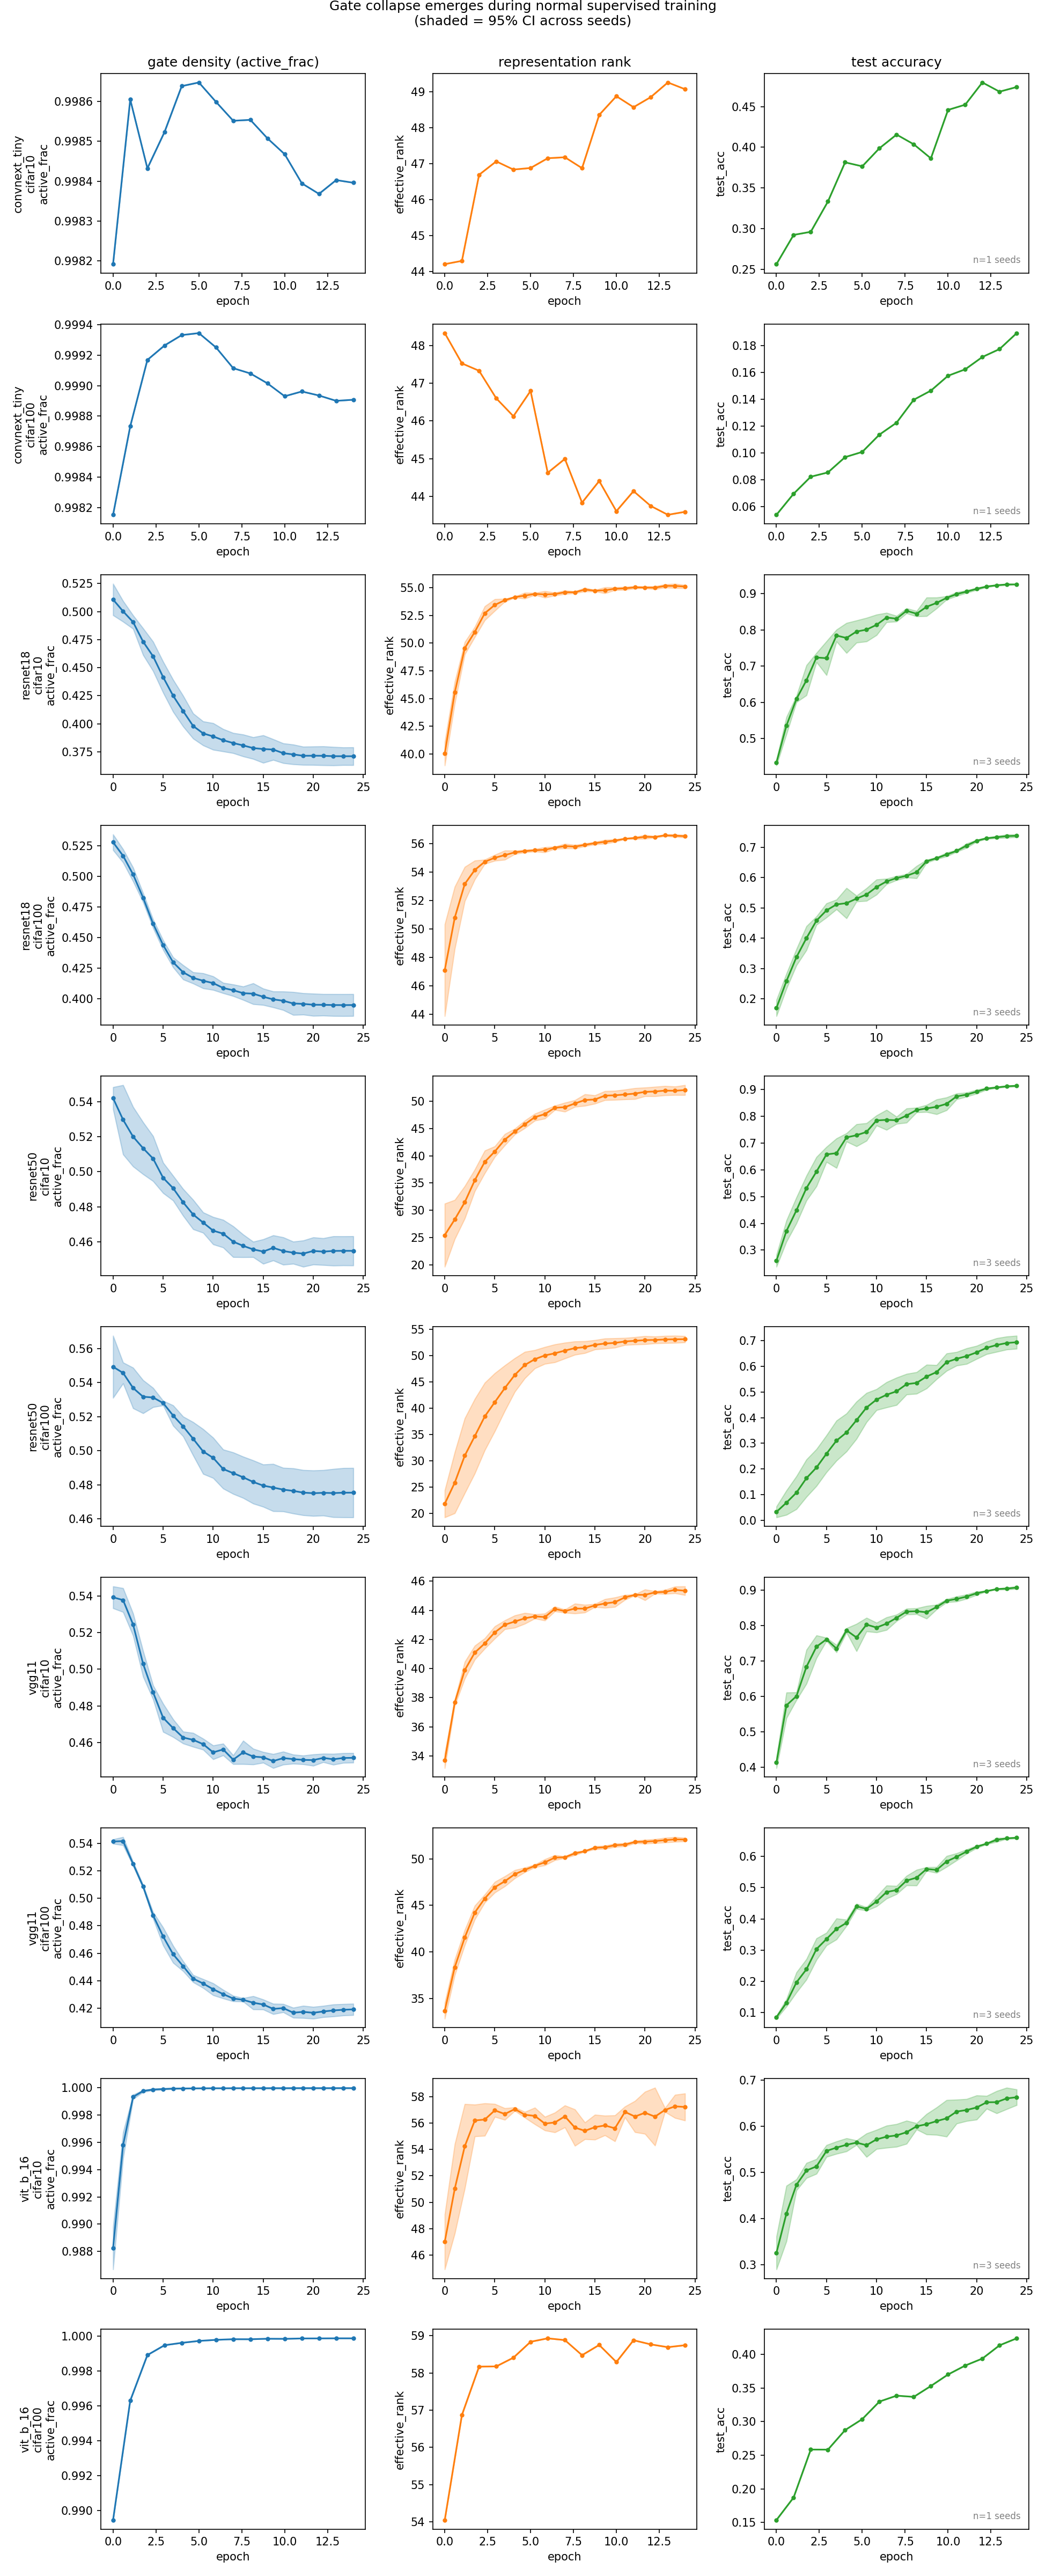
\includegraphics[width=0.92\linewidth]{training_dynamics_gate_collapse.png}
\caption{Gate collapse during normal training. Active-gradient-fraction and effective rank vs.\ epoch, ResNet-18/50/VGG-11 on CIFAR-10/100. Gate density declines and rank rises monotonically in every one of 18 trajectories.}
\label{fig:training_dynamics}
\end{figure}

This ReLU-vs-ViT contrast confounds activation with architecture family, normalization, and other structural differences. Holding ResNet-18/VGG-11 exactly fixed and swapping only the activation (ReLU, GELU, SiLU, Mish; 48 independent runs) resolves this directly: every one of 12 ReLU runs declines, every one of 12 GELU/SiLU/Mish runs rises (sign test $p=2.44\times10^{-4}$ per activation). \textbf{The direction flips with the activation, not the architecture family.} Effective rank rises in all 48 of 48 runs regardless of activation ($p=3.55\times10^{-15}$) --- it does not track the activation-class split and is reported separately as a non-discriminating observation (Section~\ref{sec:honest-nulls}).

\begin{figure}[t]
\centering
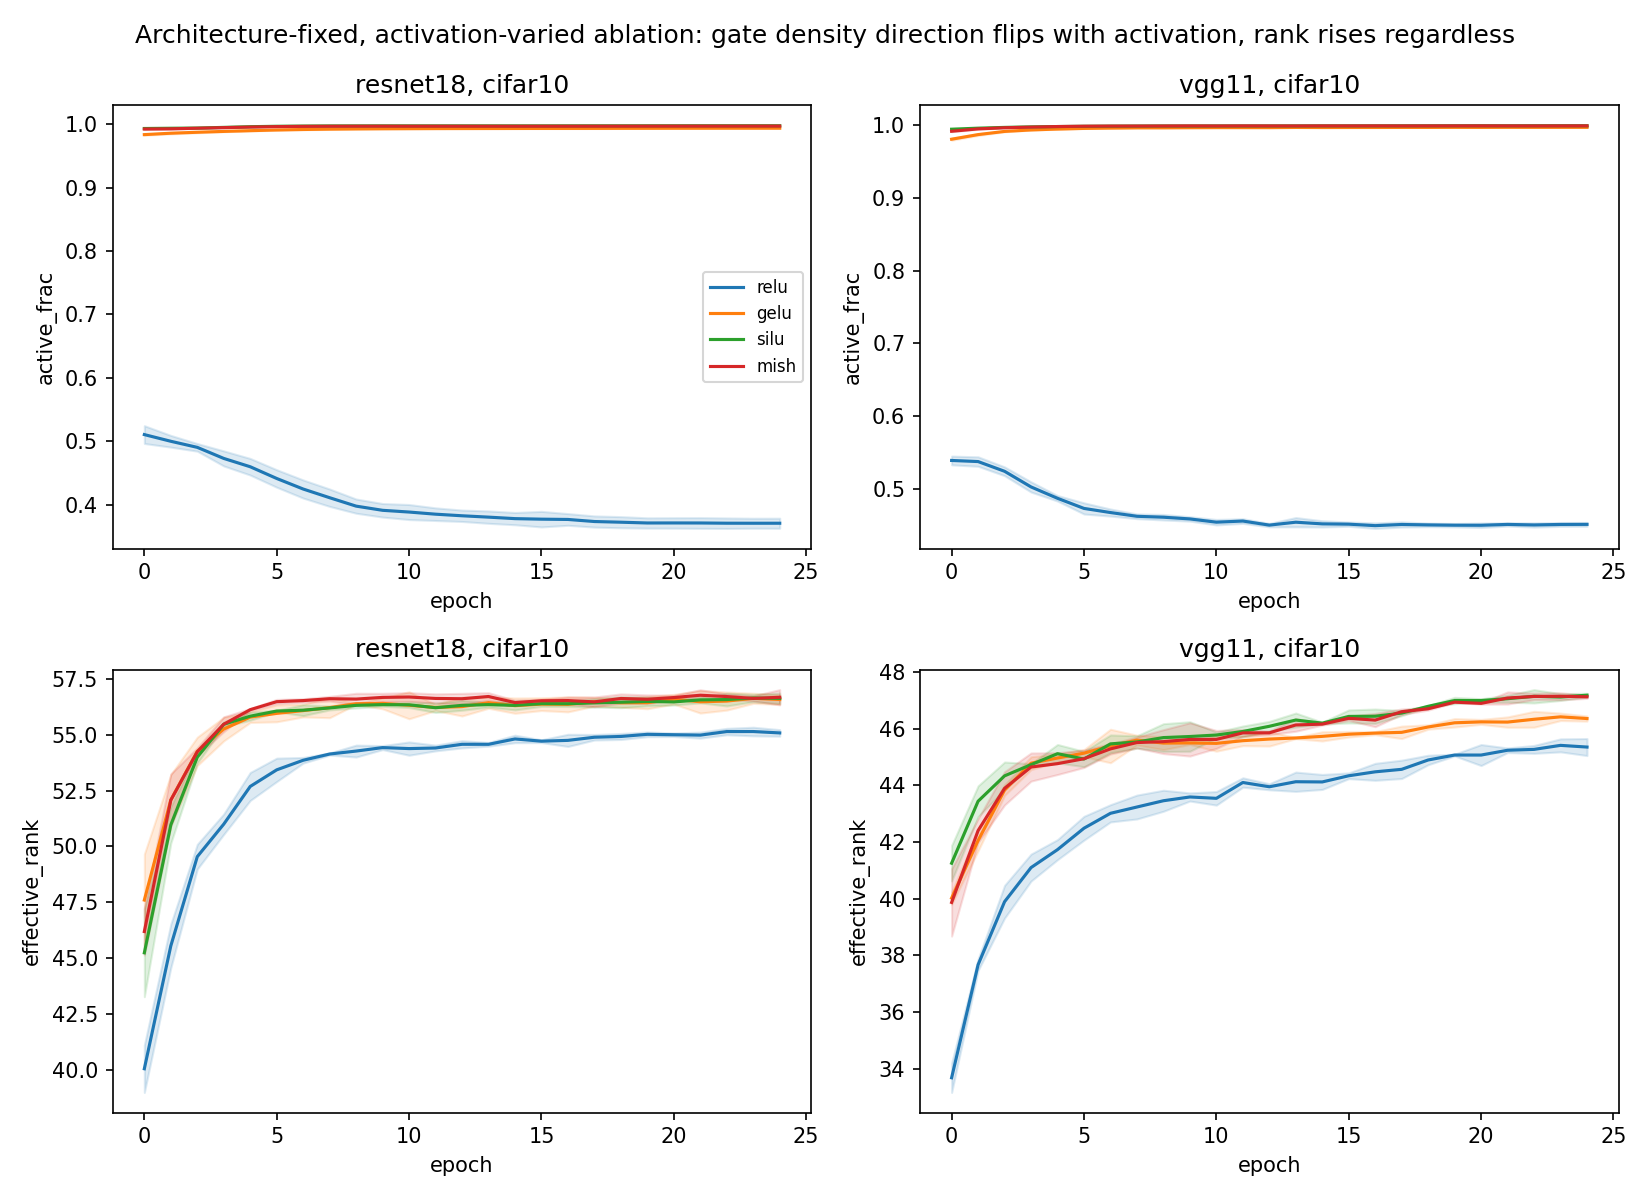
\includegraphics[width=0.92\linewidth]{activation_ablation.png}
\caption{Architecture-fixed, activation-varied ablation. Gate density falls for ReLU and rises for GELU/SiLU/Mish on the \emph{same} backbone; effective rank rises for every activation regardless of direction.}
\label{fig:activation_ablation}
\end{figure}

The direction is robust to two further checks (full detail and figures in Appendix~\ref{app:robustness}). \textbf{Normalization}: replacing every BatchNorm layer with GroupNorm on the identical ResNet-18 skeleton (4 activations, 3 seeds, 24 runs) leaves the direction unchanged --- 3 of 3 ReLU runs decline and 9 of 9 smooth-activation runs rise under \emph{both} normalization schemes --- narrowing what could be driving the phenomenon to the activation function itself, although Section~\ref{sec:mechanism} shows BatchNorm's presence specifically supplies the mechanism by which the direction is set. \textbf{Threshold}: sweeping the gate-density threshold $\theta\in\{0.001,\ldots,0.10\}$ (60 checks) gives zero sign flips, although the \emph{magnitude} of the smooth-activation rise is small at the standard threshold ($<\!1$ point against ReLU's $\sim\!13$-point fall) and grows to $+4.7$ to $+5.5$ points at the strictest threshold tested --- an asymmetry explained in Section~\ref{sec:mechanism} by quantile compression of the raw gate-value distribution (the gate-value distribution compresses from both tails toward its center for smooth activations, simultaneously raising the count above threshold while lowering the mean; ReLU's distribution remains exactly bimodal at $\{0,1\}$, so its mean and thresholded fraction must move together).

% =============================================================================
\section{Mechanism}
\label{sec:mechanism}
% =============================================================================

\subsection{A derived, tested account}
\label{sec:mechanism-derivation}

For a channel with pre-BatchNorm output $u$, BatchNorm computes
\begin{equation}
  z = \gamma \cdot \frac{u - \mathrm{mean}(u)}{\sqrt{\mathrm{var}(u)+\epsilon}} + \beta
  \;\;\Rightarrow\;\;
  \mathrm{mean}(z) \approx \beta, \quad \mathrm{var}(z) \approx \gamma^2,
\end{equation}
to first order, by BatchNorm's own definition. A convolutional layer immediately followed by BatchNorm is scale-invariant, so under SGD with weight decay its effective scale is pulled toward an equilibrium that decreases as the learning rate decays~\citep{vanlaarhoven2017l2,hoffer2018norm}; this is consistent with $\gamma$'s observed monotonic shrinkage in every one of 12 trajectories tested ($p=2.44\times10^{-4}$; $-81\%$ ReLU, $-73$ to $-74\%$ GELU/SiLU/Mish).

Define $z_{\mathrm{low}}(\theta) = \inf\{z : |f'(z)| > \theta\}$, the point where a gate crosses $\theta$ on its negative tail --- fixed and computable via automatic differentiation, no training involved. If $z\sim\mathcal{N}(\mu,\sigma^2)$ with $\sigma\to0$ and $\mu$ drifts by a \emph{similar} amount regardless of activation, then $\mathrm{active\_frac}(\theta) = P(|f'(z)|>\theta)\to0$ or $1$ depending only on which side of $z_{\mathrm{low}}(\theta)$ the shared $\mu$ lands on. We tested the shared-drift assumption directly (9 activations spanning the empirical sign transition, 3 seeds): $\mu$ flips from small-positive at initialization to a narrow, shared negative band ($-0.041$ to $-0.066$) by epoch 24 regardless of activation shape, and comparing this measured drift to each activation's independently-computed $z_{\mathrm{low}}$ predicts the observed direction in 9 of 9 cases (Appendix~\ref{app:mechanism-detail}), including correctly flagging in advance which case (closest to the boundary) should be least reliable.

\subsection{Direct per-channel verification}
\label{sec:channel_mechanism}

The test above is at the population level (one pooled $\mu$ per activation/seed/epoch). Logging per-channel $\mu_c,\sigma_c$ and active-gradient fraction for every channel of ResNet-18 (4 activations, 3 seeds, 3{,}904 channels per run), a raw per-channel margin $\mu_c - z_{\mathrm{low}}$ gives a confusing, activation-split correlation against active-gradient fraction: strong for ReLU but weakly \emph{negative} for GELU/SiLU/Mish. Diagnosis: ReLU's $z_{\mathrm{low}}$ sits within $0.03$ standard deviations of its channels' own mean (the threshold lives at the live center of the distribution), while the smooth activations' $z_{\mathrm{low}}$ sits $0.9$--$1.5$ standard deviations away; $\sigma$ shrinks $\sim\!3\times$ for every activation, while $\mu$ also drifts slightly negative for every activation. For ReLU this $\mu$-drift directly crosses the live threshold; for the smooth activations the same small $\mu$-drift instead pulls the \emph{raw} margin down even as $\sigma$'s much larger relative shrinkage pulls active-gradient fraction \emph{up} by thinning the sub-threshold tail. The raw margin conflates these forces; it does not capture $\sigma$.

Replacing the raw margin with the $\sigma$-normalized z-score $(\mu_c - z_{\mathrm{low}})/\sigma_c$ removes the confound: all four activations now show strong, uniform, positive per-channel correlation (90--96\% of channels per seed; 12 of 12 activation$\times$seed cells majority-positive, sign test $p=2.44\times10^{-4}$). \textbf{Thin-margin activations (ReLU) are driven by $\mu$ crossing a threshold at their distribution's center; thick-margin activations (GELU, SiLU, Mish) are driven by $\sigma$-shrinkage thinning a distant tail} --- two routes to the same threshold-crossing logic, unified by one $\sigma$-normalized quantity.

\begin{figure}[t]
\centering
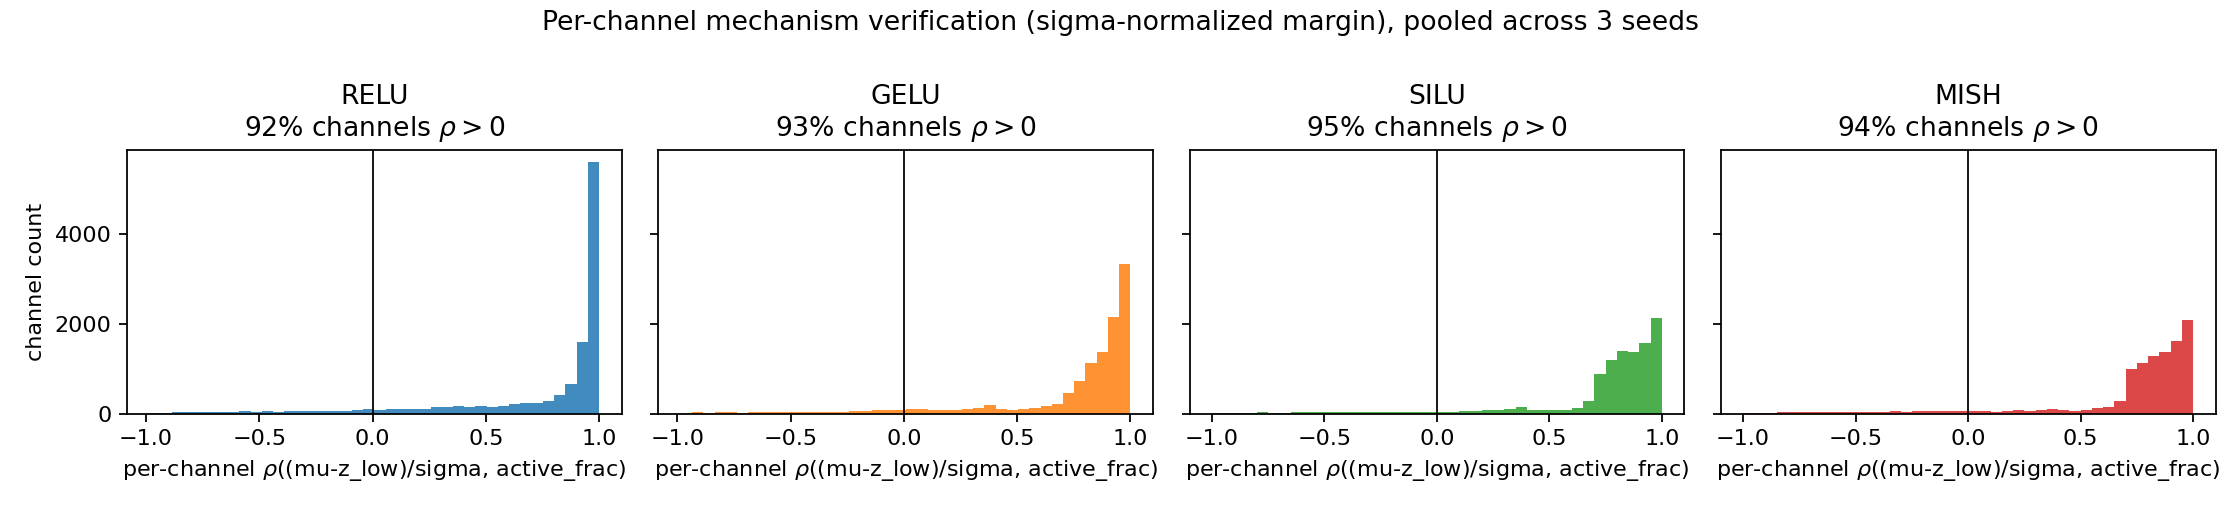
\includegraphics[width=0.95\linewidth]{channel_mechanism_zscore.png}
\caption{Per-channel verification. Histograms of the per-channel correlation between the $\sigma$-normalized margin and active-gradient fraction across 5 logged epochs, pooled over 3 seeds. All four activations show strong, uniform, positive correlation.}
\label{fig:channel_mechanism}
\end{figure}

\subsection{A unified prediction across optimizers}
\label{sec:adamw_predict}

Section~\ref{sec:optimizer} below reports that under AdamW the activation-class split collapses into a uniform decline. We treat this as a falsifiable prediction problem: \textbf{does the exact, unmodified per-channel predictor above, fed AdamW's own measured $\mu_c(t)$ and $\sigma_c(t)$, anticipate AdamW's outcome with no new free parameters?} The per-channel correlation itself remains positive under AdamW (72--90\% of channels per seed) --- expected, since the $\sigma$-normalized margin and active-gradient fraction are related through the same monotonic threshold-crossing relationship regardless of which optimizer produced the underlying $\mu,\sigma$ trajectory, so this step confirms the relationship is optimizer-invariant rather than constituting new evidence on its own. The substantive test is whether the margin's \emph{trend} matches AdamW's observed decline: for 12 of 12 activation$\times$seed cells it does (68--89\% channel-level agreement per cell; population-pooled margin deltas negative for all four activations, matching the observed active-gradient-fraction declines exactly in sign).

The mechanistic reason is direct, not inferred: per-channel $\sigma$ shrinks $\sim\!67$--$77\%$ under SGD for every activation (driving the smooth-activation rise via tail-thinning), but under AdamW it is flat for ReLU ($-0.9\%$) and \emph{grows} for every smooth activation ($+2.2$ to $+4.8\%$, Table~\ref{tab:sigma_optimizer}). With $\sigma$ flat-or-growing and $\mu$ still drifting slightly negative, the Gaussian threshold-crossing account requires the margin to decline for every activation --- which is what is observed. \textbf{This confirms the account is quantitatively faithful to AdamW's actual dynamics, not that the predictor is an oracle independent of how margin and active-gradient fraction are related}: the relationship between them is close to definitional once $\mu,\sigma,z_{\mathrm{low}}$ are fixed, and what is being tested is whether the \emph{measured inputs} (which are not fixed, and were not previously known for AdamW) take AdamW to the predicted regime. They do, in every cell tested.

\begin{table}[t]
\centering
\caption{Per-channel $\sigma$ change, epoch 0 to 24, by activation and optimizer. The mechanistic reason variance-driven activations stop rising under AdamW.}
\label{tab:sigma_optimizer}
\begin{tabular}{lcc}
\toprule
Activation & SGD & AdamW\\
\midrule
ReLU & $-77.0\%$ & $-0.9\%$ (flat)\\
GELU & $-67.5\%$ & $+2.2\%$ (grows)\\
SiLU & $-66.2\%$ & $+4.8\%$ (grows)\\
Mish & $-66.9\%$ & $+4.7\%$ (grows)\\
\bottomrule
\end{tabular}
\end{table}

\textbf{The mechanism is therefore one predictor whose governing input --- whether $\sigma$ collapses, itself set by coupled (SGD, Adam) vs.\ decoupled (AdamW) weight decay --- determines the output across every optimizer tested, rather than three disconnected, optimizer-specific observations.} A first-principles account of \emph{why} decoupling prevents $\sigma$-collapse remains open (Section~\ref{sec:limitations}).

\begin{figure}[t]
\centering
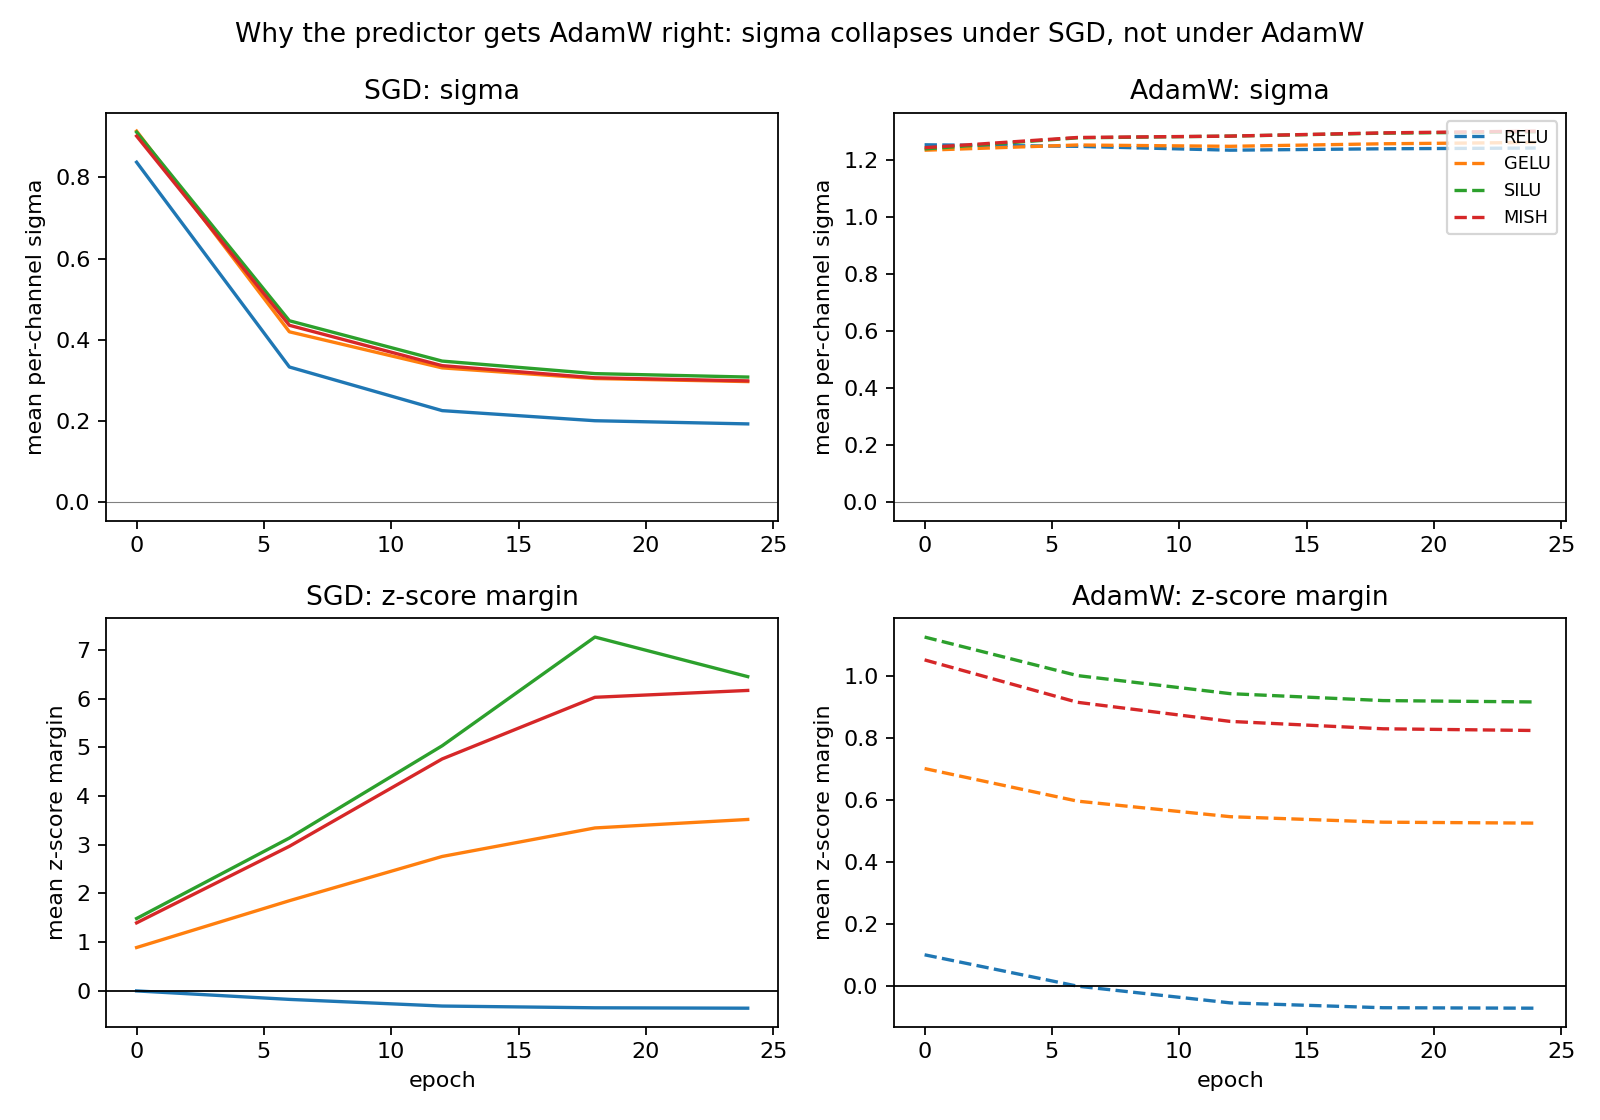
\includegraphics[width=0.85\linewidth]{adamw_prediction.png}
\caption{Why the predictor gets AdamW right. $\sigma$ collapses for every activation under SGD but is flat (ReLU) or grows (GELU/SiLU/Mish) under AdamW; the resulting margin rises for smooth activations under SGD but declines for every activation under AdamW.}
\label{fig:adamw_prediction}
\end{figure}

A 13-condition continuous smoothness sweep (ReLU; LeakyReLU at four slopes; PReLU; Softplus at $\beta\in\{50,20,10,5\}$; GELU; SiLU; Mish; 3 seeds), whose Softplus($\beta$) family has a derivative \emph{exactly} equal to the logistic sigmoid used by the originating synthetic theory (Appendix~\ref{app:synthetic}), confirms a monotonic dose-response between an initialization-time smoothness index ($\mathrm{Var}[f'(x)]$ on the fixed evaluation batch) and the observed trend (seed-level Spearman $\rho=-0.71$, $p=6\times10^{-7}$, $n=37$; condition-level $\rho=-0.73$, $p=0.0045$, $n=12$). The sign transition occurs within the Softplus($\beta$) family itself, between $\beta=50$ (decline) and $\beta=20$ (rise) --- predicted exactly by the $z_{\mathrm{low}}$ values above. One disclosed exception (PReLU, whose learned slope changes its effective smoothness during training) and the full per-condition breakdown are in Appendix~\ref{app:mechanism-detail}.

\begin{figure}[t]
\centering
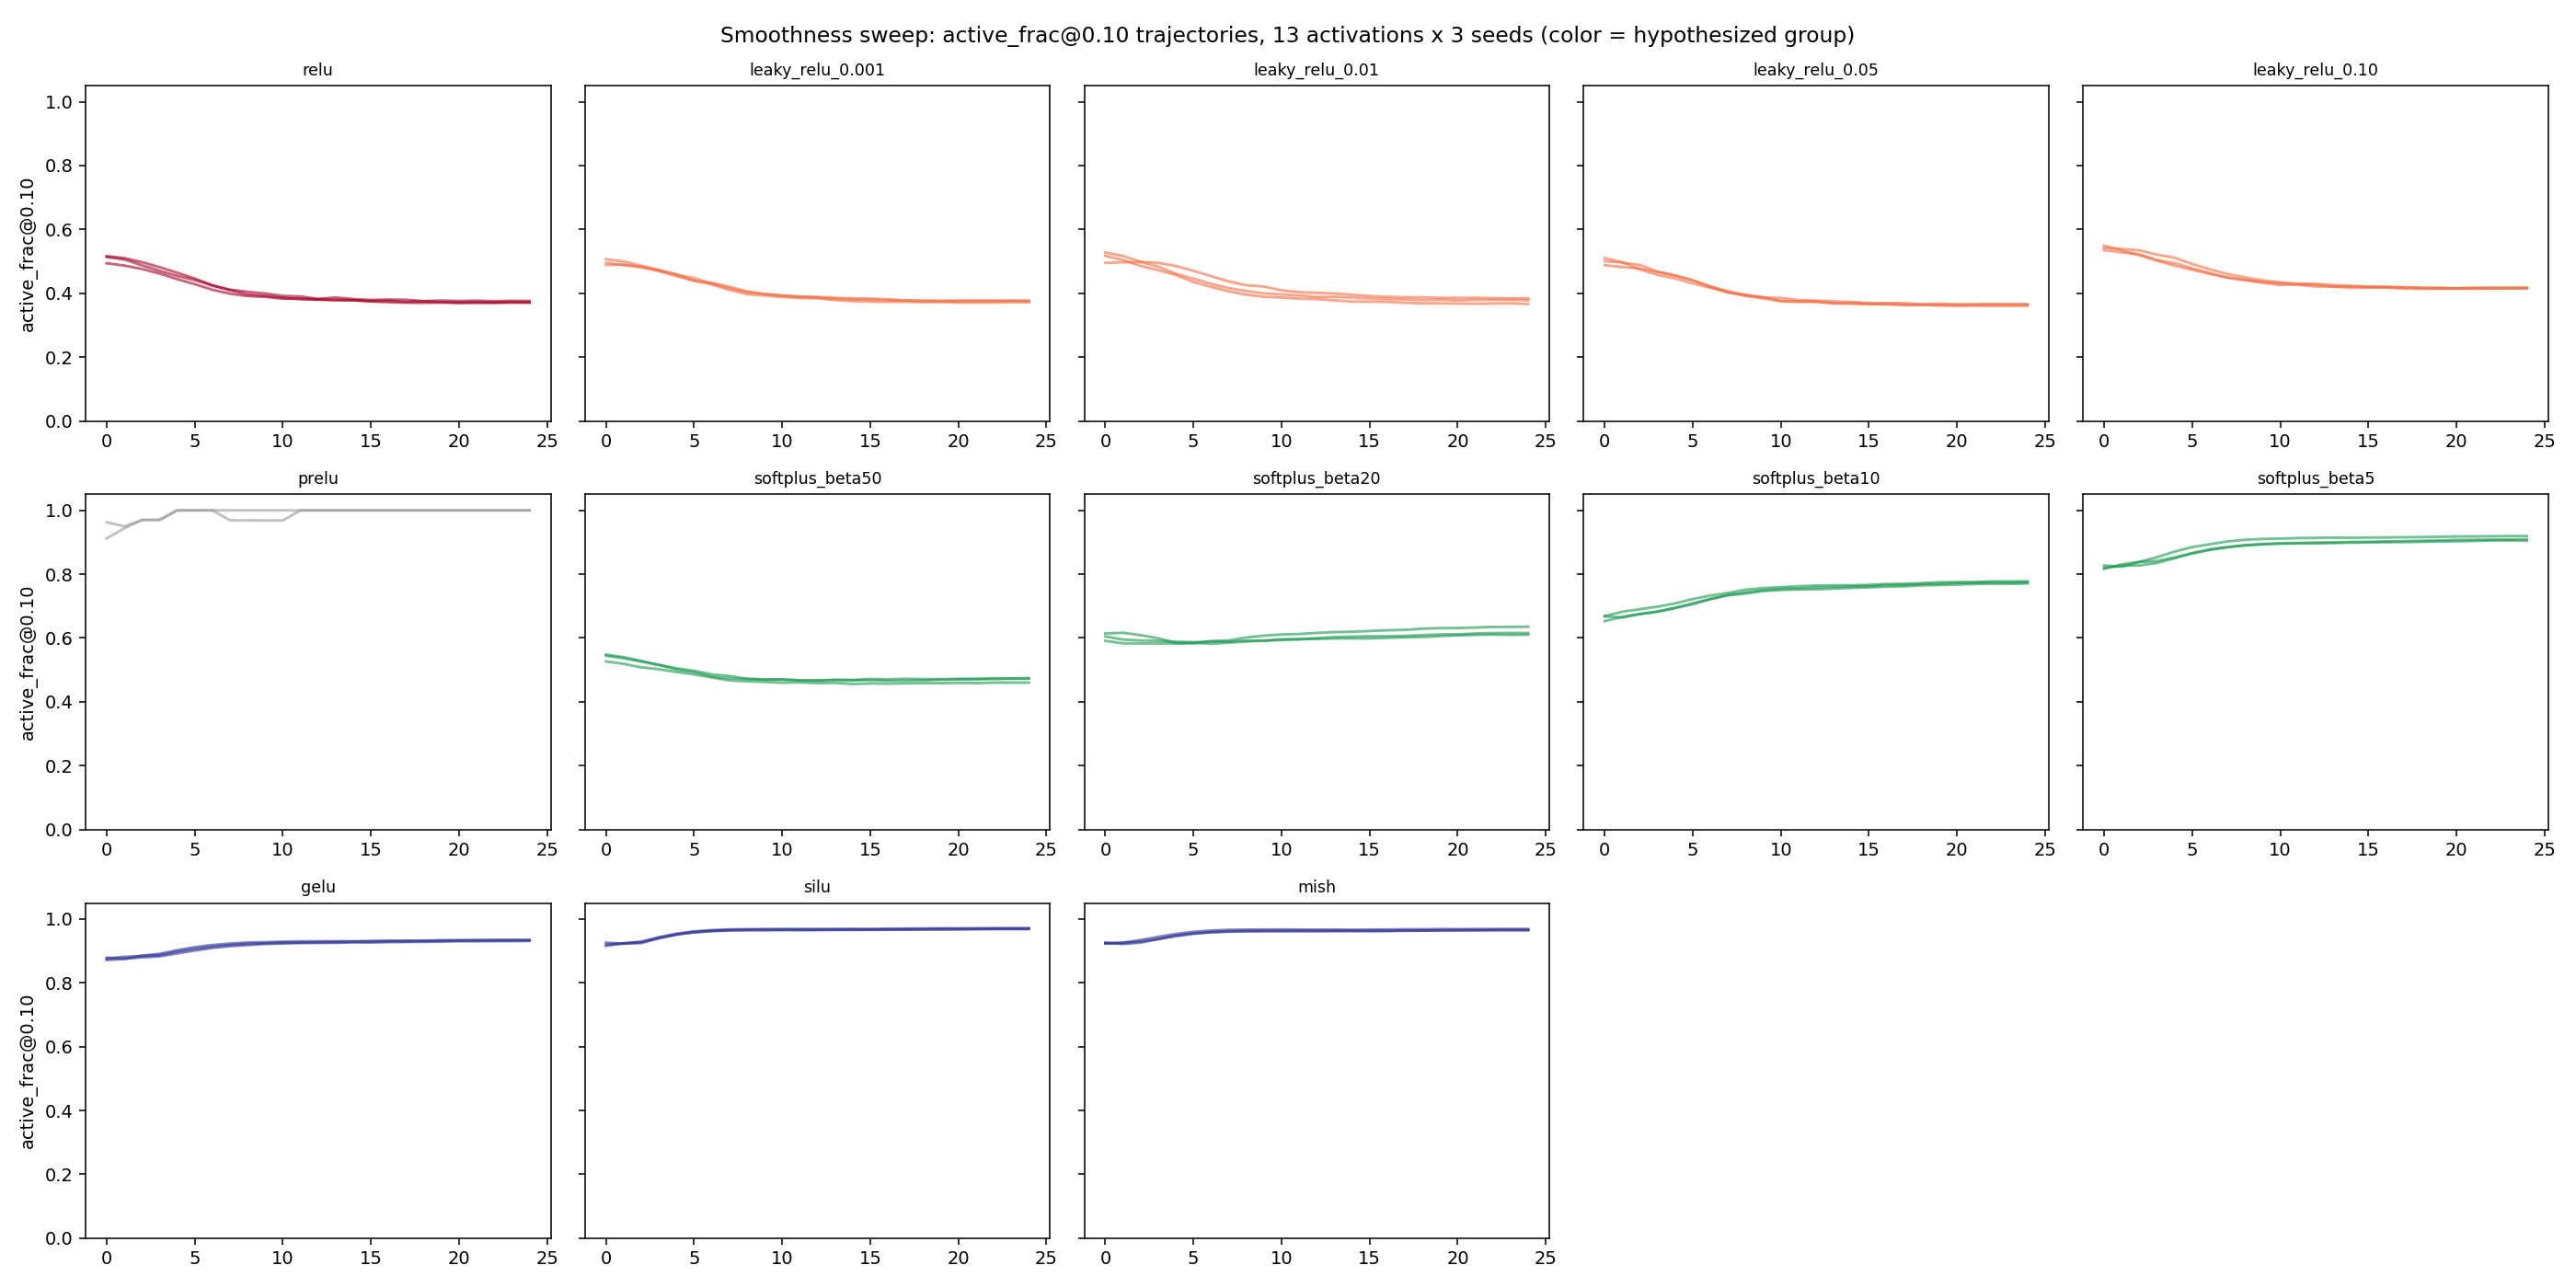
\includegraphics[width=0.92\linewidth]{smoothness_sweep_gate_dynamics.png}
\caption{Smoothness sweep. Gate-density trajectories for 13 activation conditions. The sign transition occurs within the Softplus($\beta$) family, predicted exactly by the $z_{\mathrm{low}}$ values computed independently of any training run.}
\label{fig:smoothness-main}
\end{figure}

% =============================================================================
\section{Generalization}
\label{sec:generalization}
% =============================================================================

\subsection{Optimizer}
\label{sec:optimizer}

The architecture-fixed ablation replicates exactly under Adam, coupled weight decay matching SGD's update structure (48 of 48 runs, $p=4.88\times10^{-4}$ per activation, magnitudes matching SGD). Under AdamW, decoupled weight decay, all four activations decline instead of diverging by class (48 of 48 runs, $p=4.88\times10^{-4}$) --- the pattern Section~\ref{sec:adamw_predict} shows the mechanism anticipates rather than merely accommodates.

\subsection{Scale and architecture family}

We test, rather than assume, two further axes (full detail and per-axis figures in Appendix~\ref{app:generalization-detail}). \textbf{Scale}: on Tiny-ImageNet-200 (200 classes, $64\times64$), ReLU's decline and rank-rise replicate exactly; the smooth-activation rise replicates in net displacement (9 of 9 / 8 of 9 seeds) though a whole-trajectory trend statistic loses power on this already-small effect once trajectories become non-monotonic at this scale. On a 365-class, real-photograph subsample of Places365-Standard (ResNet-50, $96\times96$, 2 seeds), the \emph{full} pattern --- large ReLU decline, small smooth-activation rise, universal rank-rise --- replicates exactly, at a class count comparable to ImageNet-1k (untested directly: registration-gated, no anonymous scriptable download). \textbf{Architecture family}: on two non-convolutional, LayerNorm-only architectures (an 8-block MLP-Mixer~\citep{tolstikhin2021mixer} and a 6-block Transformer-Encoder~\citep{vaswani2017attention}), the smooth-activation rise replicates cleanly (6 of 6 runs each, $p=0.03125$) but \textbf{the ReLU decline does not} --- it is small and architecture-dependent outside the CNN family, as is the separate universal-rank-rise observation.

\begin{figure}[t]
\centering
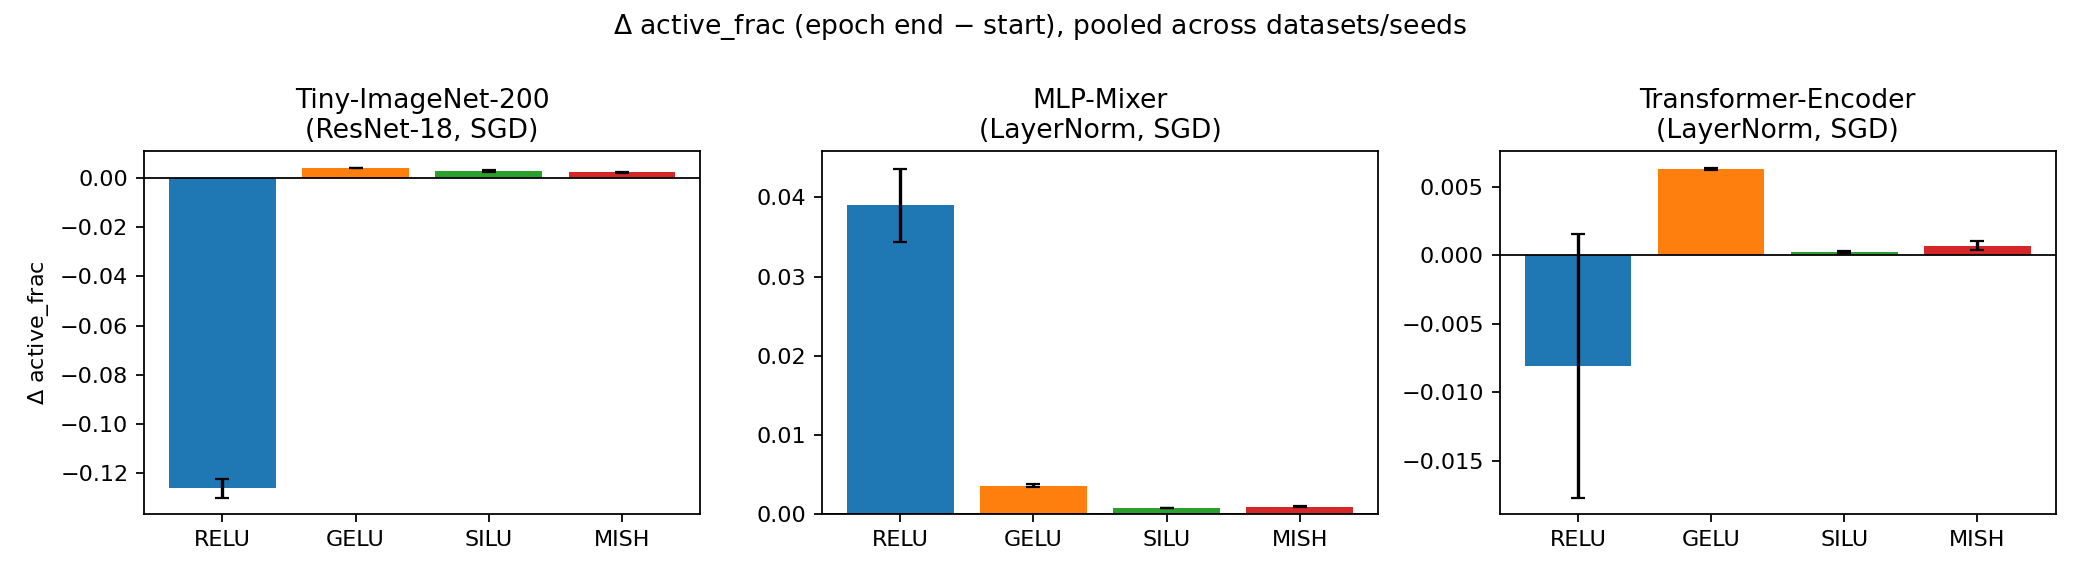
\includegraphics[width=0.98\linewidth]{generalization_scale_architecture.png}
\caption{Generalization beyond CIFAR-scale CNNs. Mean $\Delta$active-gradient-fraction, pooled across datasets/seeds. The smooth-activation rise replicates on Tiny-ImageNet-200, two non-convolutional architectures, and real photographs at 365-class scale; the ReLU decline replicates on the CNN-based experiments only.}
\label{fig:generalization}
\end{figure}

\textbf{The smooth-activation rise generalizes broadly across optimizer, scale, normalization, and architecture family; the ReLU decline and the universal-rank-rise observation are CNN-specific} --- a scope narrowing discovered by deliberately testing outside the original setup, not assumed.

% =============================================================================
\section{Honestly-Reported Non-Findings}
\label{sec:honest-nulls}
% =============================================================================

Effective rank rises in every condition tested in this paper --- 114+ independent runs regardless of activation, architecture, dataset, or threshold (pooled sign test $p<10^{-14}$) --- and has no power to discriminate anything this paper argues for; we do not list it as a contribution (full discussion, including its explicit distinction from Neural Collapse and self-supervised representation collapse, in Appendix~\ref{app:rank-pruning}).

Testing whether end-of-training gate density predicts pruning importance (ResNet-18/CIFAR-10, 4 activations, 3 seeds, global channel pruning across 1920 channels, ratios 10--70\%, no retraining), gate-density and magnitude pruning are statistically indistinguishable for ReLU (paired-$t$ $p=0.55$, an informative equivalence) but gate-density pruning is dramatically and significantly \emph{worse} than magnitude pruning for every smooth activation ($p\le1.5\times10^{-4}$; 65--80 accuracy points lost at 10\% pruning vs.\ under 1.5 for magnitude pruning, Figure~\ref{fig:pruning-main}) --- \textbf{gate density should not be used as a general-purpose channel-importance proxy}; for three of four activations tested, doing so is actively harmful (full detail in Appendix~\ref{app:rank-pruning}).

\begin{figure}[t]
\centering
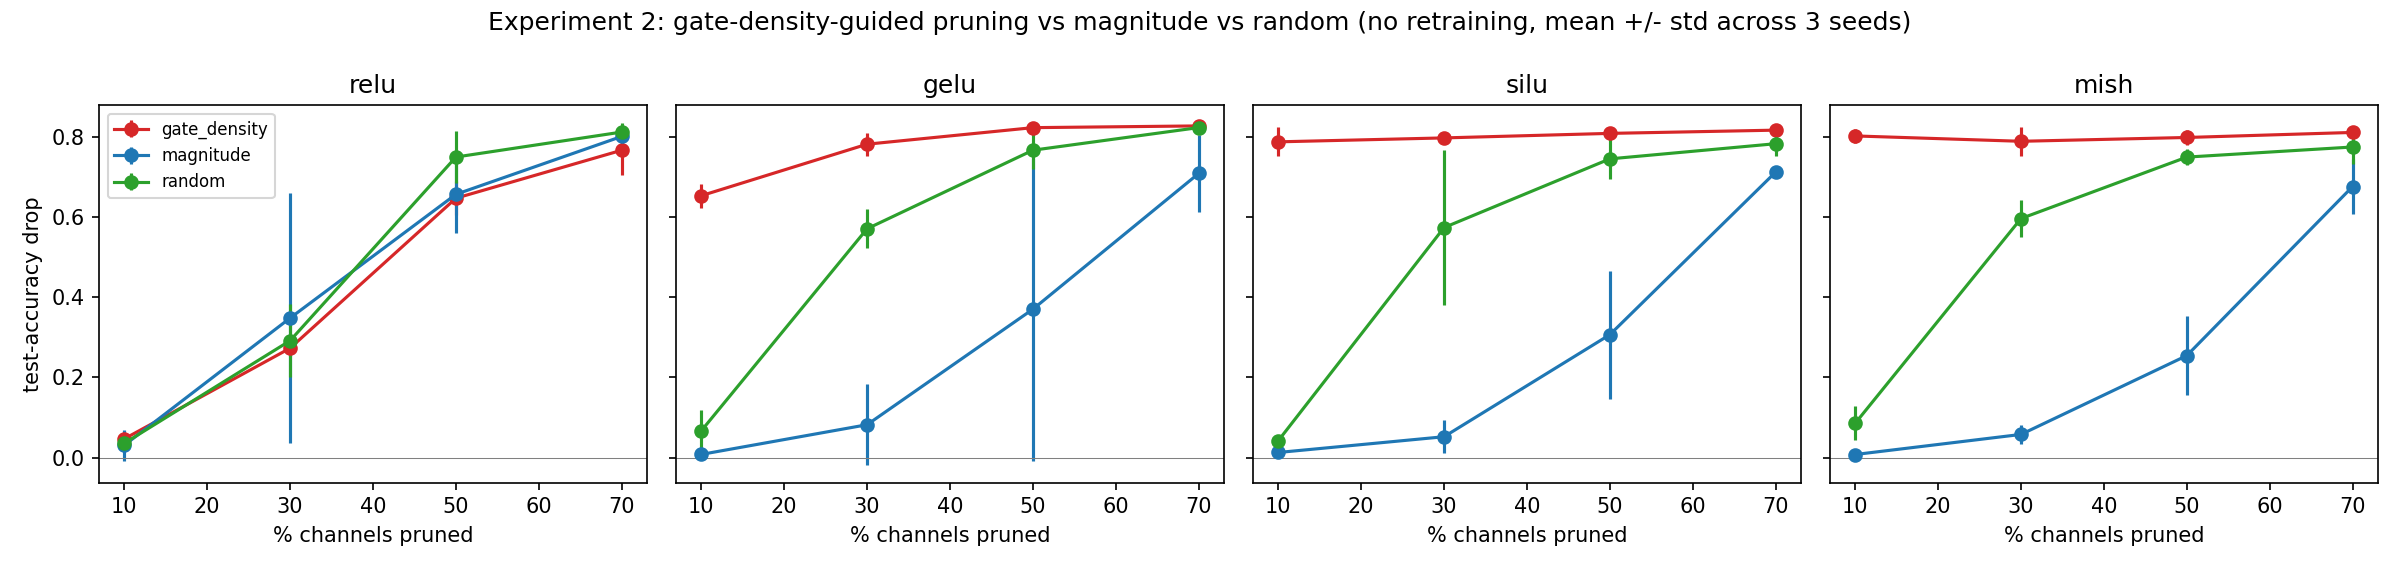
\includegraphics[width=0.85\linewidth]{pruning_accuracy_drop.png}
\caption{Gate-density-guided pruning vs.\ magnitude vs.\ random (mean $\pm$ std, 3 seeds, no retraining). Indistinguishable from magnitude pruning for ReLU; dramatically worse for every smooth activation.}
\label{fig:pruning-main}
\end{figure}

An exploratory privacy probe and a pre-registered low-data fine-tuning test are reported in full in Appendices~\ref{app:privacy} and \ref{app:payoff}: gate stiffness reduces one gradient-inversion attack's convergence but not a stronger one (attack-dependent, not a general privacy claim), and final gate density does not predict low-data fine-tuning accuracy (a genuine, pre-registered null: pooled Pearson $r=0.24$, $p=0.26$; Spearman $\rho=-0.33$, $p=0.11$, the two not even agreeing in sign).

% =============================================================================
\section{Limitations}
\label{sec:limitations}
% =============================================================================

The mechanism explains \emph{direction}, not magnitude or ultimate root cause: we do not derive a closed form for trend magnitude, and an attempted derivation of why the pre-activation mean drifts negative (Appendix~\ref{app:mechanism-detail}) accounts for the order of magnitude of the shared drift but not its residual, statistically real cross-activation variation. We do not have a first-principles account of why AdamW's decoupled weight decay specifically prevents $\sigma$-collapse, only that it empirically does and that the mechanism correctly anticipates the consequence. ConvNeXt-Tiny is excluded from all claims (undertrained, inconsistent rank sign across datasets; Appendix~\ref{app:generalization-detail}). Architecture families beyond CNNs, MLP-Mixer, and Transformer-Encoder remain untested, as does full-scale ImageNet-1k directly.

% =============================================================================
\section{Conclusion}
% =============================================================================

Gate density diverges by activation class during ordinary training under coupled-weight-decay optimizers, and this divergence is derived, not asserted: BatchNorm's scale shrinks under weight decay, collapsing pre-activation variance for every activation alike, and whether this collapse drives gate density toward 0 or 1 depends only on a fixed, activation-specific threshold-crossing point, verified at the population level, the individual-channel level, and across a continuous smoothness sweep. The decisive test is predictive rather than merely descriptive: fed a different optimizer's (AdamW's) own measured statistics, the identical mechanism anticipates a qualitatively different, uniform-decline outcome with zero new free parameters, because decoupled weight decay prevents the variance collapse the mechanism's first step requires. The smooth-activation half of this finding generalizes broadly across optimizer, scale, and architecture family; the ReLU-specific decline and a separate rank-rise observation are CNN-specific. We report, rather than omit, every place this story does not extend cleanly. The result is a bounded, mechanistically-derived and mechanistically-\emph{predictive} account of activation-class-dependent gate dynamics --- not a universal theory of gradient dynamics, and we do not claim it as one.

\begin{ack}
\end{ack}

\section*{References}
{\small
\begin{thebibliography}{99}

\bibitem{lu2019dying}
Lu, L., Shin, Y., Su, Y., and Karniadakis, G.\,E. (2019).
Dying ReLU and initialization: theory and numerical examples.
\textit{Communications in Computational Physics}, 28(5), 1671--1706.

\bibitem{glorot2010understanding}
Glorot, X. and Bengio, Y. (2010).
Understanding the difficulty of training deep feedforward neural networks.
\textit{Proceedings of AISTATS}, 249--256.

\bibitem{frankle2019lottery}
Frankle, J. and Carbin, M. (2019).
The lottery ticket hypothesis: finding sparse, trainable neural networks.
\textit{International Conference on Learning Representations (ICLR)}.

\bibitem{dong2021attention}
Dong, Y., Cordonnier, J.-B., and Loukas, A. (2021).
Attention is not all you need: pure attention loses rank doubly
exponentially with depth.
\textit{International Conference on Machine Learning (ICML)}.

\bibitem{papyan2020prevalence}
Papyan, V., Han, X.\,Y., and Donoho, D.\,L. (2020).
Prevalence of neural collapse during the terminal phase of deep learning
training.
\textit{Proceedings of the National Academy of Sciences}, 117(40),
24652--24663.

\bibitem{hua2021feature}
Hua, T., Wang, W., Xue, Z., Ren, S., Wang, Y., and Zhao, H. (2021).
On feature decorrelation in self-supervised learning.
\textit{International Conference on Computer Vision (ICCV)}.

\bibitem{jing2022understanding}
Jing, L., Vincent, P., LeCun, Y., and Tian, Y. (2022).
Understanding dimensional collapse in contrastive self-supervised learning.
\textit{International Conference on Learning Representations (ICLR)}.

\bibitem{zhao2020idlg}
Zhao, B., Mopuri, K.\,R., and Bilen, H. (2020).
iDLG: improved deep leakage from gradients.
\textit{arXiv preprint arXiv:2001.02610}.

\bibitem{geiping2020inverting}
Geiping, J., Bauermeister, H., Dr\"oge, H., and Moeller, M. (2020).
Inverting gradients---how easy is it to break privacy in federated
learning?
\textit{Advances in Neural Information Processing Systems}, 33.

\bibitem{vanlaarhoven2017l2}
van Laarhoven, T. (2017).
L2 regularization versus batch and weight normalization.
\textit{arXiv preprint arXiv:1706.05350}.

\bibitem{hoffer2018norm}
Hoffer, E., Banner, R., Golan, I., and Soudry, D. (2018).
Norm matters: efficient and accurate normalization schemes in deep
networks.
\textit{Advances in Neural Information Processing Systems}, 31.

\bibitem{tolstikhin2021mixer}
Tolstikhin, I., Houlsby, N., Kolesnikov, A., Beyer, L., Zhai, X.,
Unterthiner, T., Yung, J., Steiner, A., Keysers, D., Uszkoreit, J.,
Lucic, M., and Dosovitskiy, A. (2021).
MLP-Mixer: an all-MLP architecture for vision.
\textit{Advances in Neural Information Processing Systems}, 34.

\bibitem{vaswani2017attention}
Vaswani, A., Shazeer, N., Parmar, N., Uszkoreit, J., Jones, L.,
Gomez, A.\,N., Kaiser, L., and Polosukhin, I. (2017).
Attention is all you need.
\textit{Advances in Neural Information Processing Systems}, 30.

\bibitem{zhu2019deep}
Zhu, L., Liu, Z., and Han, S. (2019).
Deep leakage from gradients.
\textit{Advances in Neural Information Processing Systems}, 32.

\bibitem{donoho2006compressed}
Donoho, D.\,L. (2006).
Compressed sensing.
\textit{IEEE Transactions on Information Theory}, 52(4), 1289--1306.

\end{thebibliography}
}

\appendix
\section{Technical Appendices and Supplementary Material}

This appendix is supplementary: the main text stands on its own. Every
result summarized in the main text is given in full here, with the exact
numbers, figures, and experimental detail that did not fit the 9-page
limit.

\subsection{Method detail: validation and architecture-fixed ablation}
\label{app:method-detail}

We validate the gate-recovery method against the only available ground
truth --- ReLU's known $\approx\!50\%$ active-fraction at
BatchNorm-normalized random initialization --- across 20 seeds and three
architectures (Table~\ref{tab:init_profile}).

\begin{table}[h]
\centering
\caption{Active-gradient-fraction at random initialization, 20 seeds,
$\theta=0.01$. ReLU architectures cluster near the theoretical $\approx 50\%$
expectation; GELU-based architectures are near-ceiling; ViT-B/16 shows
vanishing gradients at default initialization (resolved as an
initialization artifact below, not a property of depth).}
\label{tab:init_profile}
\begin{tabular}{lcc}
\toprule
Architecture & Mean active-fraction & Std\\
\midrule
ResNet-18 & 0.555 & 0.156\\
ResNet-50 & 0.529 & 0.116\\
VGG-11 & 0.618 & 0.141\\
ConvNeXt-Tiny & 0.994 & 0.004\\
ViT-B/16 & NaN (vanishing at init) & ---\\
\bottomrule
\end{tabular}
\end{table}

\paragraph{The ViT-B/16 vanishing-gradient finding is an initialization
artifact, not depth-related.} A dedicated falsification sweep across depth
(1--12 layers), initialization scheme (default vs.\ truncated-normal
$\mathrm{std}=0.02$), and batch size (4--64), replicated independently
twice, finds gradients vanish in 100\% of seeds at \emph{every} depth under
default initialization and in 0\% of seeds at every depth under the
standard fix. This is unrelated to, and should not be conflated with, the
training-time direction split studied in the main paper.

\paragraph{Architecture-fixed activation ablation, method.} To separate
activation effects from architecture effects (Section~\ref{sec:dynamics}),
we hold the ResNet-18 and VGG-11 skeletons exactly fixed --- identical
depth, width, stem, BatchNorm placement, and parameter count, verified
identical across activations --- and vary only the activation module via a
single constructor argument. The same mechanism extends to the
BatchNorm-versus-GroupNorm ablation in Appendix~\ref{app:robustness}
(replacing every \texttt{BatchNorm2d} with \texttt{GroupNorm}, 32 groups or
fewer for narrow layers) on the identical skeleton.

\subsection{BatchNorm and threshold robustness}
\label{app:robustness}

Replacing every BatchNorm layer with GroupNorm on the identical ResNet-18
skeleton (4 activations, 3 seeds, 24 runs) leaves the direction unchanged:
3 of 3 ReLU runs decline and 9 of 9 smooth-activation runs rise under
\emph{both} normalization schemes (Figure~\ref{fig:bn_ablation}). Magnitude
is noisier under GroupNorm, particularly for Mish, and final accuracy is
$\sim$2--4 points lower --- both attributable to GroupNorm being unmatched
in hyperparameters at this scale, not evidence about the underlying
mechanism. BatchNorm is not a necessary condition for the phenomenon,
narrowing what could be driving it to the activation function itself ---
though Section~\ref{sec:mechanism} shows BatchNorm's presence \emph{does}
supply the specific mechanism by which the direction is set in the main
experiments.

\begin{figure}[h]
\centering
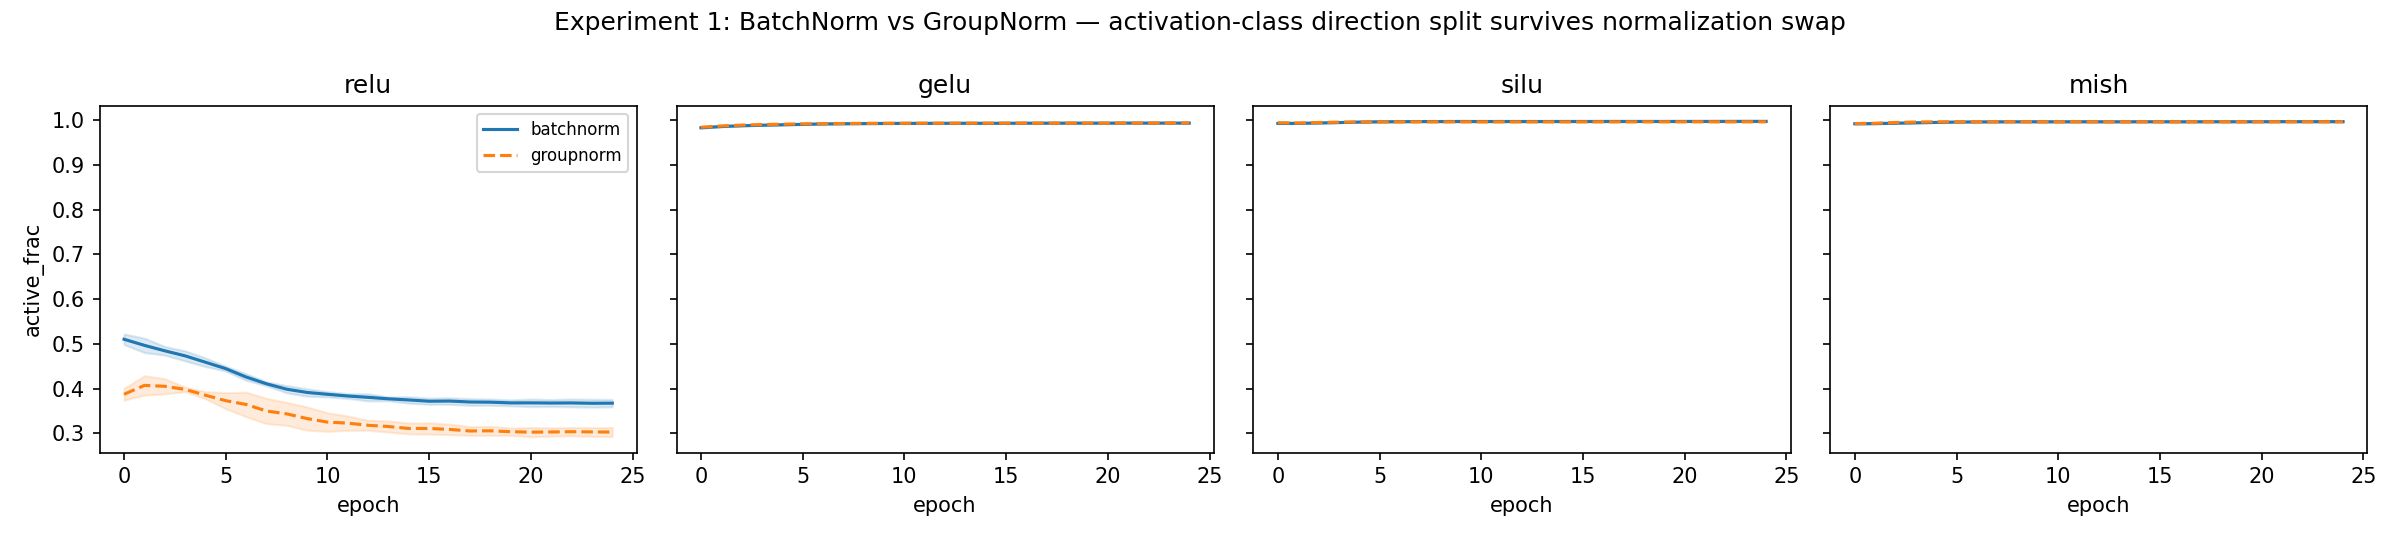
\includegraphics[width=0.92\linewidth]{bn_vs_gn_gate_dynamics.png}
\caption{BatchNorm vs.\ GroupNorm. The activation-class direction split
(ReLU declining, smooth activations rising) is identical under both
normalization schemes, on the identical ResNet-18 skeleton.}
\label{fig:bn_ablation}
\end{figure}

The active-gradient-fraction statistic depends on a threshold $\theta$.
Sweeping $\theta\in\{0.001,0.005,0.01,0.05,0.10\}$ on the architecture-fixed
ResNet-18 ablation (4 activations, 3 seeds, 60 checks) finds zero sign
flips: ReLU declines and every smooth activation rises at every threshold
tested. The magnitude of the effect is asymmetric: at the originally-used
threshold ($\theta=0.01$), the smooth-activation rise is small in absolute
terms ($<1$ percentage point) against ReLU's $\sim$13-point fall; the
effect becomes comparably large only at the strictest threshold tested
($\theta=0.10$: $+4.7$ to $+5.5$ points).

\begin{figure}[h]
\centering
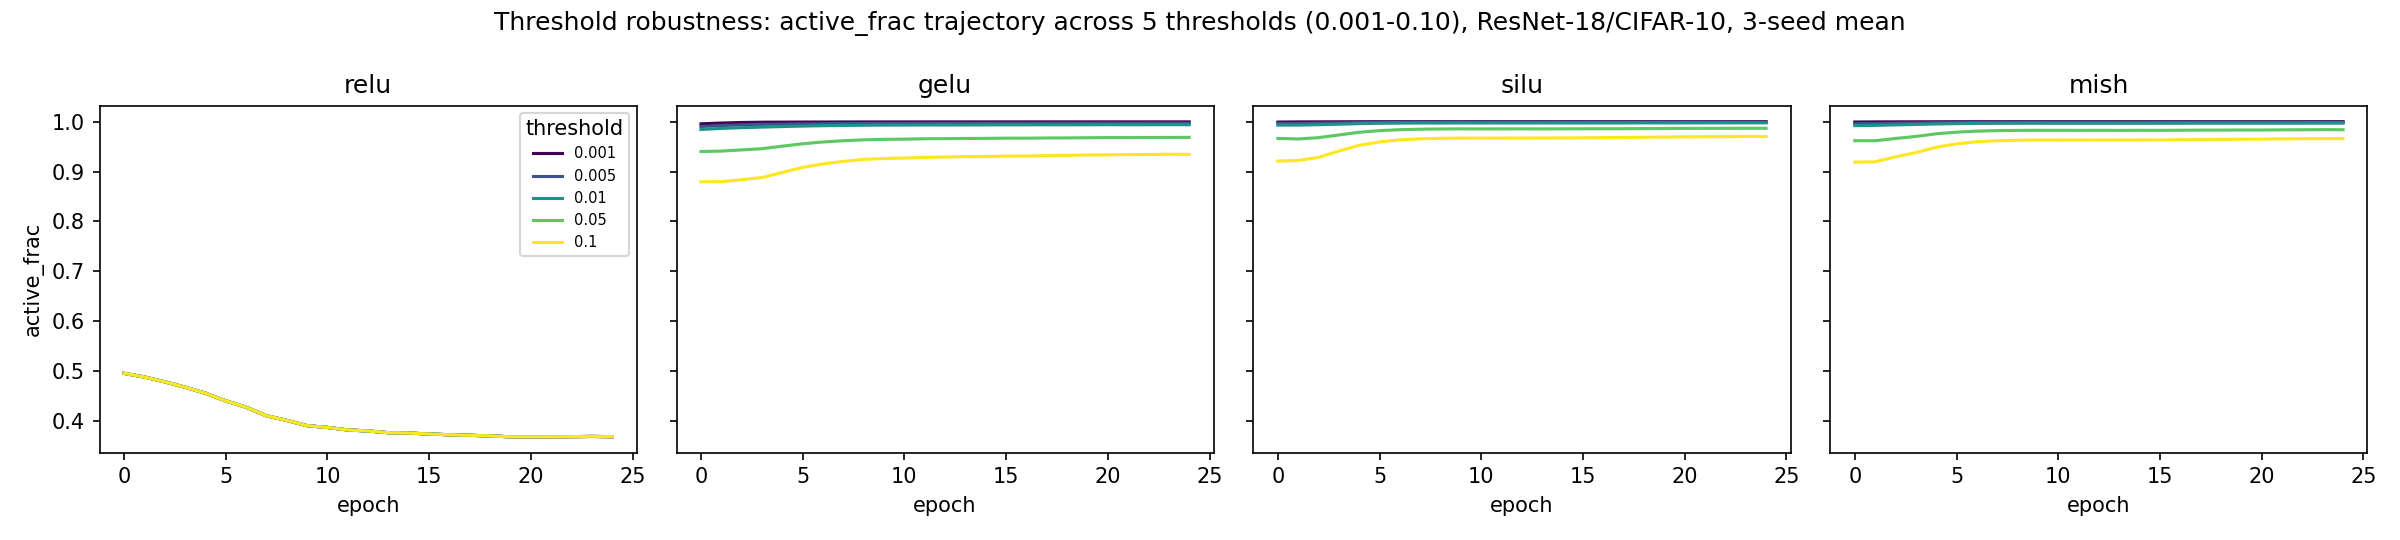
\includegraphics[width=0.95\linewidth]{threshold_robustness.png}
\caption{Threshold robustness. Active-gradient-fraction trajectories across
five thresholds spanning two orders of magnitude. ReLU declines and every
smooth activation rises at every threshold; magnitude grows with stricter
thresholds.}
\label{fig:threshold_robustness}
\end{figure}

The raw, threshold-free gate magnitude (\texttt{gate\_mean}) declines for
every activation tested, including the ones whose thresholded gate density
rises (ReLU $-25.5\%$, GELU $-15.3\%$, SiLU $-9.0\%$, Mish $-8.4\%$). This
is not a contradiction: per-channel quantile analysis shows the gate-value
distribution compresses from both tails toward its center for smooth
activations (e.g.\ GELU's 5th percentile rises from 0.041 to 0.076 while
its 95th percentile falls from 1.10 to 0.88 over training), simultaneously
raising the count above a near-zero threshold while lowering the mean;
ReLU's distribution remains exactly bimodal at $\{0,1\}$ throughout, so its
mean and thresholded fraction are mathematically identical and must move
together. Section~\ref{sec:mechanism} explains why this compression happens
for every activation but produces opposite threshold-crossing outcomes.

\begin{figure}[h]
\centering
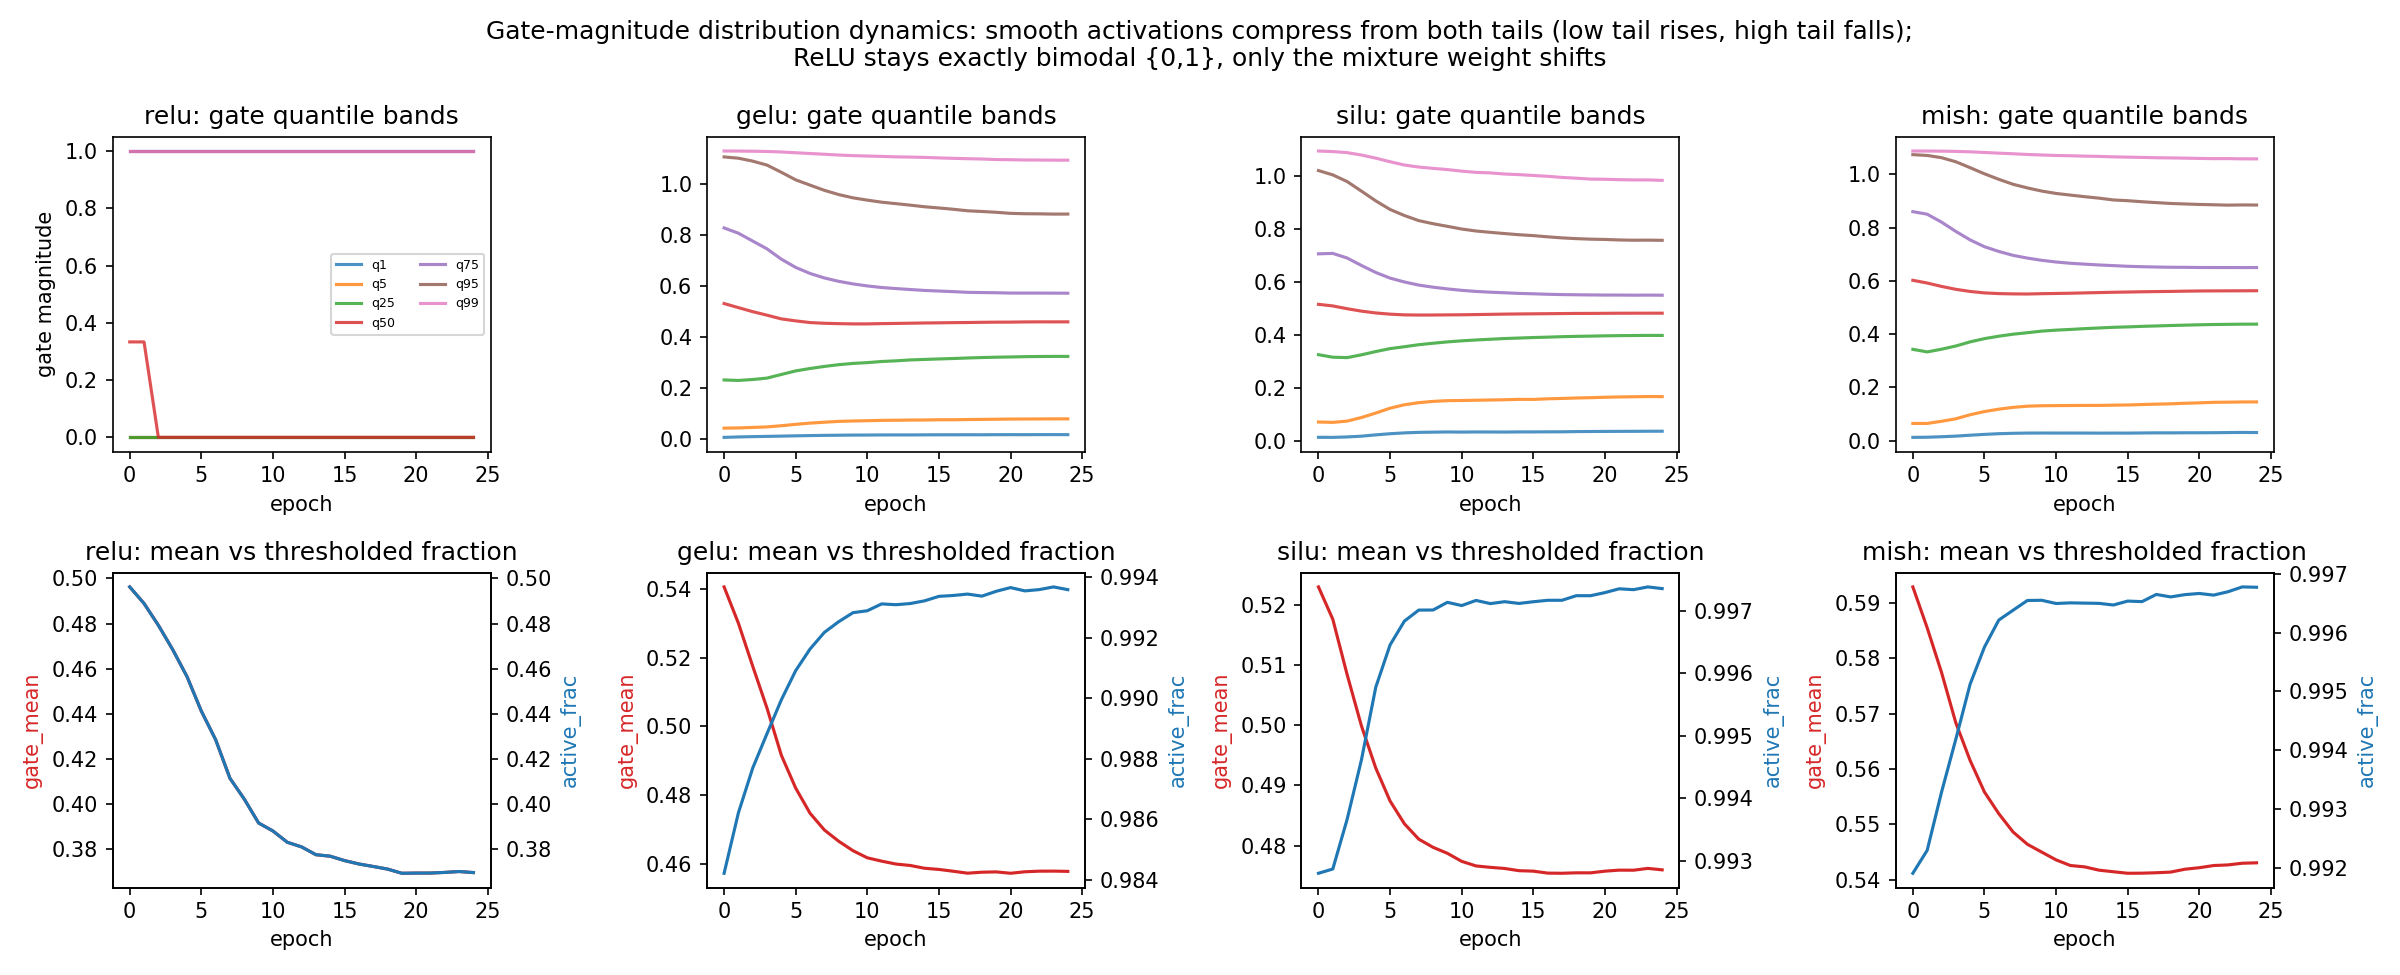
\includegraphics[width=0.95\linewidth]{gate_distribution_dynamics.png}
\caption{Gate-magnitude distribution dynamics. Quantile bands (1st--99th
percentile) over training, by activation. Smooth activations compress from
both tails toward a moderate center; ReLU remains exactly bimodal
$\{0,1\}$, with training only shifting the mixture weight between modes.}
\label{fig:gate_distribution}
\end{figure}

\begin{figure}[h]
\centering
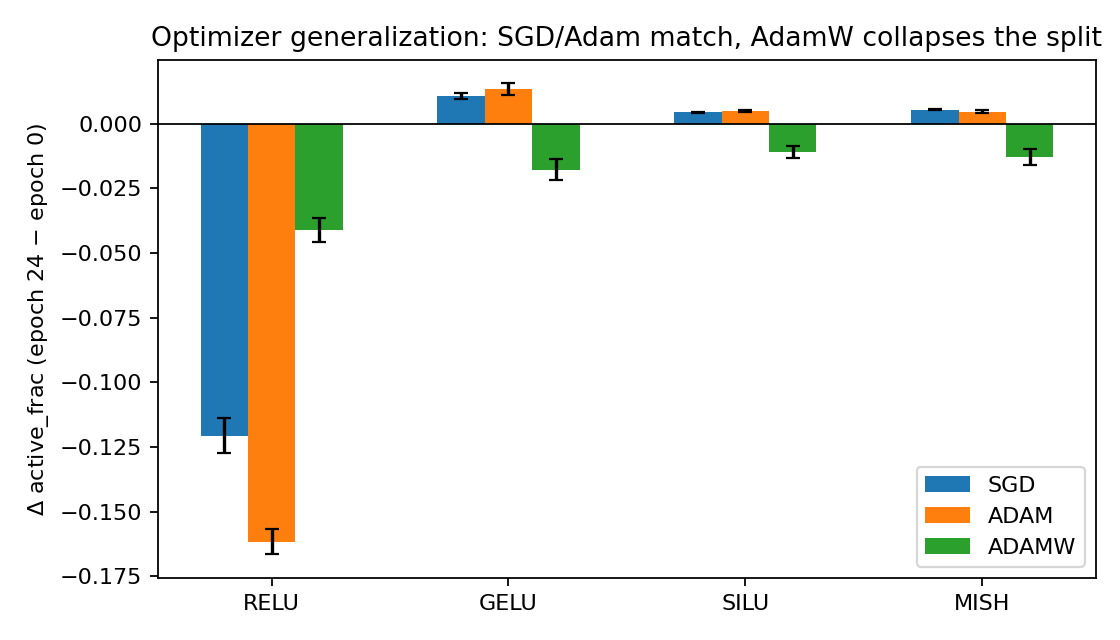
\includegraphics[width=0.85\linewidth]{optimizer_generalization.png}
\caption{Optimizer generalization. Mean $\Delta$active-gradient-fraction
(epoch 24 minus epoch 0), by activation and optimizer, $\pm$ standard error
across 12 independent runs. SGD and Adam (both coupled weight decay) give
the same direction split; AdamW (decoupled weight decay) gives a uniform
decline instead --- the pattern Section~\ref{sec:adamw_predict} shows the
mechanism predicts exactly, with no new free parameters.}
\label{fig:optimizer_generalization}
\end{figure}

\subsection{Mechanism detail: threshold-crossing table, shared-drift test, smoothness sweep, and the mu-drift derivation}
\label{app:mechanism-detail}

Table~\ref{tab:zlow} gives $z_{\rm low}(\theta=0.10)$, computed exactly via
automatic differentiation, against the empirically observed gate-density
trend.

\begin{table}[h]
\centering
\caption{$z_{\rm low}(\theta=0.10)$, computed exactly via autograd, vs.\
the empirically observed gate-density trend.}
\label{tab:zlow}
\begin{tabular}{lccc}
\toprule
Activation & $z_{\rm low}$ & Observed $\rho$(epoch, gate density) & Direction\\
\midrule
ReLU / LeakyReLU (all slopes) & $0.000$ & $-0.96$ to $-0.99$ & decline\\
Softplus $\beta=50$ & $-0.044$ & $-0.59$ & decline\\
Softplus $\beta=20$ & $-0.110$ & $+0.73$ & rise\\
Softplus $\beta=10$ & $-0.219$ & $+1.00$ & rise\\
Softplus $\beta=5$ & $-0.439$ & $+1.00$ & rise\\
GELU & $-0.554$ & $+1.00$ & rise\\
SiLU & $-0.912$ & $+0.99$ & rise\\
Mish & $-0.891$ & $+0.97$ & rise\\
\bottomrule
\end{tabular}
\end{table}

We tested the shared-drift assumption rather than assuming it: logging
signed pre-activation mean (forward-hook only, no backward pass) for 9
representative activations spanning the transition, 3 seeds, 25 epochs. At
initialization $\mu$ is small and positive for every activation
($0.014$--$0.033$); by epoch 6 it has flipped negative for every single
activation tested and remains in a narrow, shared band through epoch 24:
$-0.041$ (SiLU) to $-0.066$ (Mish) --- a common drift, not nine separate
trajectories.

\begin{table}[h]
\centering
\caption{Mechanism validation: predicted vs.\ observed direction, derived
from the measured shared $\mu$-drift and the independently-computed
$z_{\rm low}$. 9 of 9 predictions correct.}
\label{tab:mechanism_validation}
\begin{tabular}{lccccc}
\toprule
Activation & $\mu$(epoch 24) & $z_{\rm low}$ & Margin & Predicted & Match\\
\midrule
ReLU & $-0.0458$ & $0.000$ & $-0.0458$ & decline & \checkmark\\
LeakyReLU(0.01) & $-0.0478$ & $0.000$ & $-0.0478$ & decline & \checkmark\\
Softplus $\beta=50$ & $-0.0476$ & $-0.044$ & $-0.0036$ & decline & \checkmark\\
Softplus $\beta=20$ & $-0.0568$ & $-0.110$ & $+0.0532$ & rise & \checkmark\\
Softplus $\beta=10$ & $-0.0635$ & $-0.219$ & $+0.1555$ & rise & \checkmark\\
Softplus $\beta=5$ & $-0.0586$ & $-0.439$ & $+0.3804$ & rise & \checkmark\\
GELU & $-0.0508$ & $-0.554$ & $+0.5032$ & rise & \checkmark\\
SiLU & $-0.0413$ & $-0.912$ & $+0.8707$ & rise & \checkmark\\
Mish & $-0.0655$ & $-0.891$ & $+0.8255$ & rise & \checkmark\\
\bottomrule
\end{tabular}
\end{table}

\begin{figure}[h]
\centering
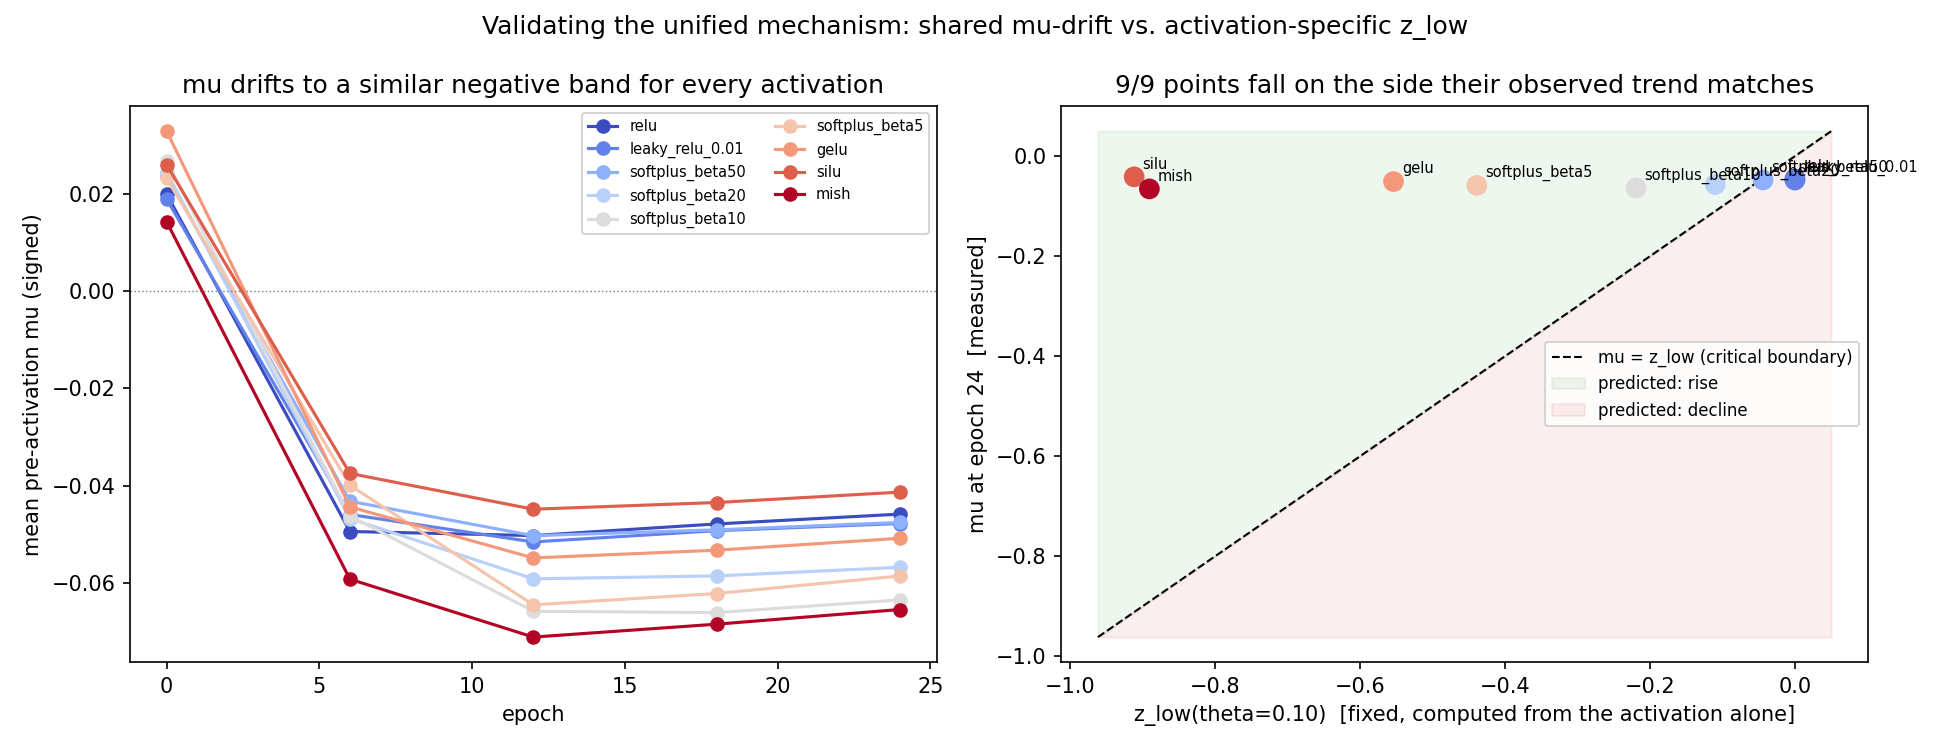
\includegraphics[width=0.92\linewidth]{theory_mechanism_validation.png}
\caption{Mechanism validation. (Left) Pre-activation mean drifts to a
shared negative band across 9 different activation functions. (Right)
Plotting each activation's measured $\mu$ against its independently
computed $z_{\rm low}$: every point falls on the side its observed trend
matches. Softplus($\beta=50$) sits within $0.0036$ of the critical
boundary --- the one condition with a conspicuously weak, high-variance
empirical correlation ($\rho=-0.59$ vs.\ $|\rho|>0.96$ elsewhere), which the
mechanism correctly anticipates.}
\label{fig:mechanism_validation}
\end{figure}

\paragraph{Smoothness sweep.}
\label{sec:smoothness}
Softplus's derivative is exactly the logistic
sigmoid, $\mathrm{softplus}'(x;\beta)=\mathrm{sigmoid}(\beta x)$ --- the same
gate formalism used by the originating synthetic theory
(Appendix~\ref{app:synthetic}), with $\beta$ playing the role of that
theory's stiffness parameter $\alpha$; this is an exact mathematical
correspondence, not an analogy. A 13-condition sweep (ReLU; LeakyReLU at
four slopes; PReLU; Softplus at $\beta\in\{50,20,10,5\}$; GELU; SiLU; Mish;
3 seeds; 25 epochs) tests whether smoothness predicts the trend in a
continuous dose-response, using $\mathrm{Var}[f'(x)]$ at initialization on
the fixed evaluation batch as a smoothness index (trajectories plotted in
Figure~\ref{fig:smoothness-main} in the main text).

\begin{figure}[h]
\centering
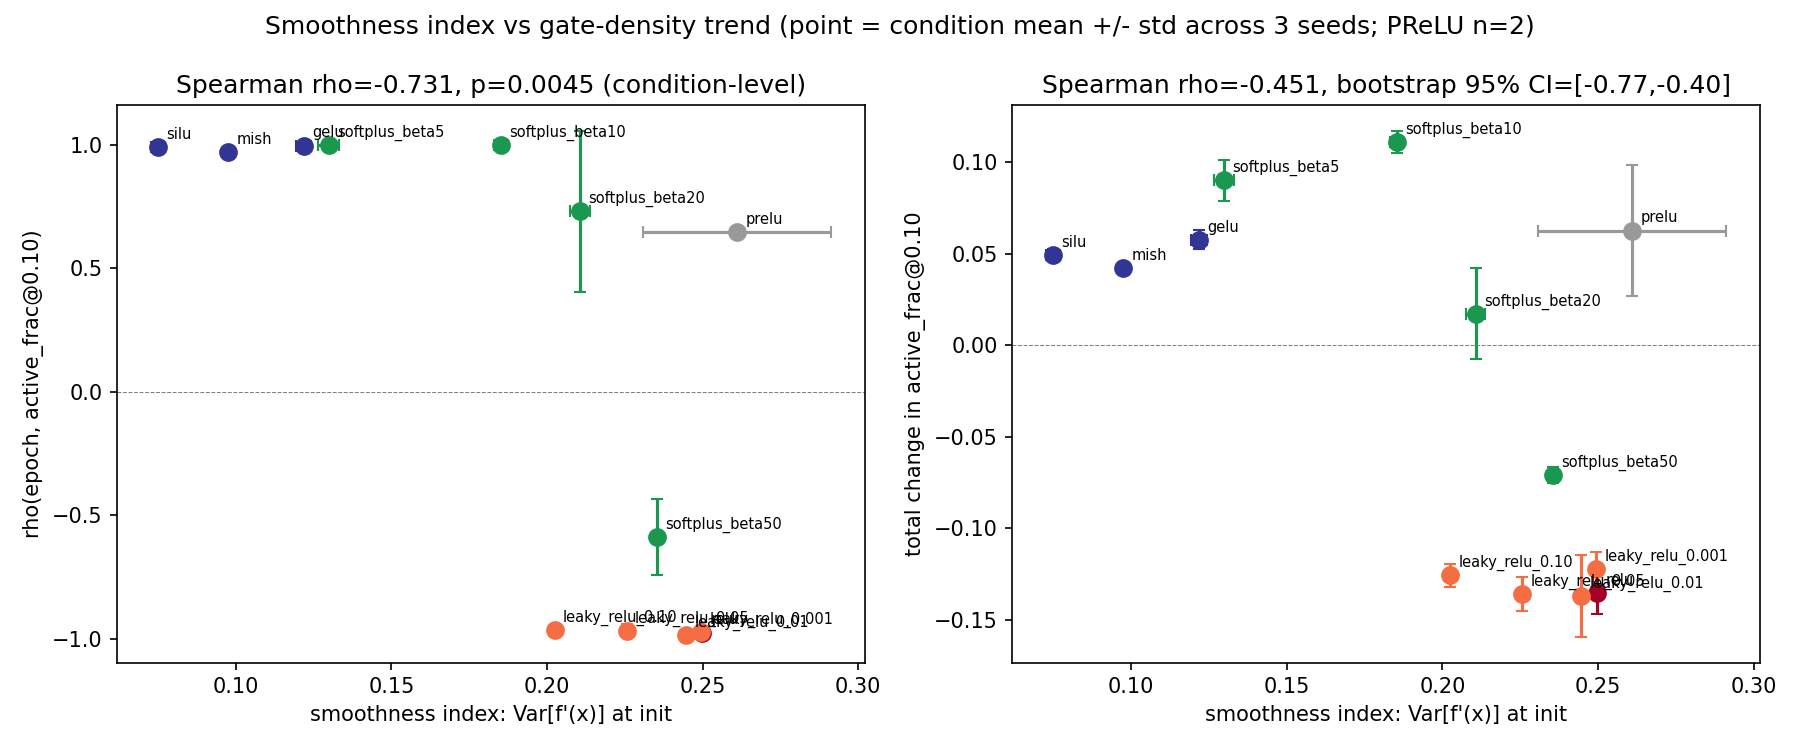
\includegraphics[width=0.92\linewidth]{smoothness_vs_gate_trend.png}
\caption{Smoothness index vs.\ gate-density trend. Spearman
$\rho=-0.731$, $p=0.0045$ (condition-level, $n=12$); $\rho=-0.710$,
$p=6.1\times10^{-7}$ (seed-level, $n=37$). One excluded point: PReLU
seed~0 failed to train (10\% accuracy throughout, NaN gate statistics from
epoch 0) and is disclosed, not silently dropped.}
\label{fig:smoothness_correlation}
\end{figure}

The relationship is significant at the seed-trajectory level for both
trend shape ($\rho=-0.710$, $p=6.1\times10^{-7}$) and magnitude
($\rho=-0.605$, $p=5.7\times10^{-5}$), and at the condition level for
trend shape ($\rho=-0.731$, $p=0.0045$); the condition-level magnitude
correlation does not individually reach $p<0.05$ at $n=12$ ($p=0.122$) but
its bootstrap 95\% CI, $[-0.775,-0.401]$, excludes zero. PReLU is a genuine
exception: its smoothness index at initialization (0.261) is the highest
of all 13 conditions, yet it rises. This reflects a limitation of measuring
smoothness only at initialization: PReLU's negative-slope parameter is
learned and its effective smoothness changes substantially during training
(gate variance falls from $\sim$0.24--0.28 to $\sim$0.08--0.12), unlike
fixed-shape activations.

\paragraph{The mu-drift derivation.} The mechanism above explains direction
given that $\mu$ drifts negative; it does not explain \emph{why}. This
project's optimizer applies weight decay to every parameter, including
BatchNorm's $\beta$. For a parameter evolving under plain SGD with weight
decay, $\theta_{t+1} = \theta_t - \eta(g_t + \lambda\theta_t)$, where $g_t$
is the task gradient and $\lambda$ the decay coefficient: if $g_t$ has a
roughly-constant average value $\bar g$ over a window where $\eta$ is
locally constant, the system relaxes toward a quasi-equilibrium
$\theta^\ast \approx -\bar g/\lambda$. For BatchNorm's $\beta$, $g_t =
dL/d\beta = \sum_{\text{batch}} dL/dz$ --- the gradient flowing into the
pre-activation, summed over the batch. This is a generic fact about SGD
with L2 regularization, not specific to BatchNorm's scale-invariance (unlike
the $\gamma$ argument, which needs scale-invariance specifically). The
falsifiable prediction: if $\bar g$ is set mainly by the shared
architecture/task rather than by each activation's own shape, $\beta$'s
equilibrium value should be nearly identical across very different
activation functions (same $\lambda=5\times10^{-4}$ for all) and should not
correlate with activation-specific shape properties like $z_{\rm low}$ or
an initialization-time smoothness index.

Tested against the same 9-activation drift data above: $\mu$ at epoch 24
ranges only $-0.065$ to $-0.041$ (spread $0.024$) across activations whose
$z_{\rm low}$ spans $-0.00005$ to $-1.234$ (four orders of magnitude) ---
the narrowness this account predicts. The cross-activation variation is
nonetheless statistically real: one-way ANOVA across the 9 activations,
$F=29.7$, $p=7.7\times10^{-9}$; between-activation standard deviation
(0.0084) is $3.5\times$ the within-activation (seed) standard deviation
(0.0024). This residual variation does not correlate with $z_{\rm low}$
(Pearson $r=0.26$, $p=0.51$; Spearman $\rho=0.28$, $p=0.46$) nor with the
initialization-time smoothness index (Pearson $r=0.15$, $p=0.71$; Spearman
$\rho=0.30$, $p=0.43$). The equilibrium argument correctly predicts the
order of magnitude of the shared drift band and gives it a mechanistic
reason (shared $\lambda$, roughly shared $\bar g$) rather than leaving it
as an unexplained empirical regularity; it does not explain the residual,
statistically significant cross-activation variation within that band. We
tested two natural candidates and stopped rather than searching for a
third that fits.

\subsection{Generalization detail: scale, architecture family, and ConvNeXt}
\label{app:generalization-detail}

\paragraph{Tiny-ImageNet-200.} ResNet-18 (the existing CIFAR-native stem,
which keeps an $8\times8$ feature map before the global pool at
$64\times64$ resolution rather than collapsing it prematurely), 200
classes, $64\times64$, 100k training images, 4 activations, 3 seeds, 25
epochs. ReLU's decline and effective-rank rise replicate exactly (6 of 6
seed-level checks across both metrics, matching CIFAR in direction and
magnitude). The smooth activations' smaller-magnitude rise also replicates
in net displacement for 9 of 9 (active-gradient fraction) and 8 of 9
(effective rank) seeds, but the trajectories are no longer monotonic at
this scale --- an early overshoot followed by partial relaxation --- so a
whole-trajectory linear-trend statistic loses power on this already-small
effect even though net direction is preserved; we report both statistics
rather than the more favorable one alone.

\paragraph{Places365-Standard.} ResNet-50 (same CIFAR-native stem family,
$96\times96$ input, $12\times12$ feature map before the global pool), a
fixed, seeded 150-train/20-val-per-class subsample (365 scene classes,
real, uncurated photographs, comparable in class count to ImageNet-1k,
which we did not test directly --- it requires registration and has no
anonymous scriptable download), 4 activations, 2 seeds (disclosed as 2,
not the usual 3, for compute-budget reasons), 25 epochs. Every seed-level
check agrees with the established direction by both the trend and
net-displacement statistics: ReLU declines (2 of 2 seeds, $-6.7$ to
$-8.3$ points) while GELU, SiLU, and Mish all rise (2 of 2 seeds each,
$+0.3$ to $+1.1$ points) --- the same large-decline, small-rise asymmetry
seen throughout this paper. Effective rank rises for all four activations,
consistent with ResNet-50 remaining a CNN. With only 2 seeds the sign test
cannot exceed $p=0.5$; this experiment adds a real-photograph,
larger-class-count replication, not independent statistical power beyond
what the other CNN experiments already establish.

\paragraph{Architecture family.} Two CIFAR-native, activation-configurable,
non-convolutional architectures with no BatchNorm anywhere: an 8-block
MLP-Mixer~\citep{tolstikhin2021mixer} and a 6-block, 4-head
Transformer-Encoder~\citep{vaswani2017attention} (patch size 4, hidden
dimension 128, $\sim$1M parameters each), both LayerNorm-only, instrumented
with the same gate-recovery hooks (every activation is an explicit
submodule, unlike \texttt{nn.TransformerEncoderLayer}'s functional
activation, which the hook-based recovery cannot see). Same 4 activations,
both datasets, 3 seeds, 25 epochs. GELU, SiLU, and Mish all rise robustly
in both new architectures (6 of 6 independent runs each, sign test
$p=0.03125$, magnitude $+0.1$ to $+0.8$ points). The ReLU decline does not
generalize: it rises in 5 of 6 MLP-Mixer runs, and is small and
dataset-dependent in the Transformer-Encoder (mildly declining on
CIFAR-100, mixed on CIFAR-10), with nothing resembling the large, robust
CNN decline. Effective rank is the most architecture-dependent statistic of
all: MLP-Mixer's rank \emph{declines} for every activation including ReLU,
and the Transformer-Encoder's rank splits by activation (ReLU rises, the
smooth activations decline).

\paragraph{ConvNeXt-Tiny: excluded from all claims.} A single-seed,
15-epoch training-dynamics run on CIFAR-10 (47.4\% final test accuracy)
showed effective rank rising (consistent with other smooth activations);
the corresponding CIFAR-100 run, badly undertrained at 18.9\% final
accuracy, showed effective rank \emph{falling}. We attribute the sign
disagreement to undertraining, not a real architectural effect, and
exclude ConvNeXt-Tiny from every quantitative claim in this paper.

\subsection{Representational rank and pruning, in full}
\label{app:rank-pruning}

\paragraph{Representational rank: a null result.} Effective rank rises in
every condition tested in this paper --- all 18 original trajectories, all
48 architecture-ablation runs, all 24 BatchNorm/GroupNorm runs, regardless
of activation, architecture, dataset, or threshold (114+ independent runs,
sign test $p<10^{-14}$ pooled). A statistic that moves in the same
direction in every condition tried has no power to discriminate anything
this paper argues for, and we do not list it as a contribution. We flag,
but do not resolve, a possible connection to BatchNorm-statistics dynamics
(Section~\ref{sec:mechanism}), and explicitly distinguish it from Neural
Collapse~\citep{papyan2020prevalence} (different layer, different
training-phase window) and self-supervised representation
collapse~\citep{hua2021feature,jing2022understanding} (opposite sign,
unrelated mechanism).

\paragraph{Pruning: gate density is not a general-purpose importance
signal.} We tested whether end-of-training gate density predicts channel
importance for pruning, using the same ResNet-18/CIFAR-10 checkpoints (4
activations, 3 seeds, global channel pruning across 1920 channels in 8
layers, ratios 10--70\%, no retraining, compared against magnitude pruning
and a random baseline; full per-ratio results plotted in
Figure~\ref{fig:pruning-main} in the main text).

For ReLU, gate-density and magnitude pruning are statistically
indistinguishable (paired-$t$ $p=0.55$) --- informative equivalence. For
GELU, SiLU, and Mish, gate-density pruning is significantly worse than
magnitude pruning at every ratio ($p=1.5\times10^{-4}$,
$5.2\times10^{-5}$, $2.3\times10^{-5}$ respectively): at 10\% pruning,
removing the lowest-gate-density channels costs 65--80 accuracy points,
while removing the lowest-magnitude channels costs under 1.5 points. Gate
density should not be presented or used as a general-purpose proxy for
channel importance; for three of the four activations studied, doing so is
actively harmful, not merely uninformative.

\subsection{Exploratory privacy probe, in full}
\label{sec:privacy}
\label{app:privacy}

As one possible consequence of gate dynamics, we ask whether gate density
affects gradient-inversion attack success, using a controllable victim
model (a small CNN with one tunable-stiffness sigmoid gate, distinct from
the real architectures studied above) against
DLG~\citep{zhu2019deep}, iDLG~\citep{zhao2020idlg}, and the stronger,
scale-invariant Inverting Gradients attack~\citep{geiping2020inverting} (7
stiffness values, 20 seeds).

\begin{figure}[h]
\centering
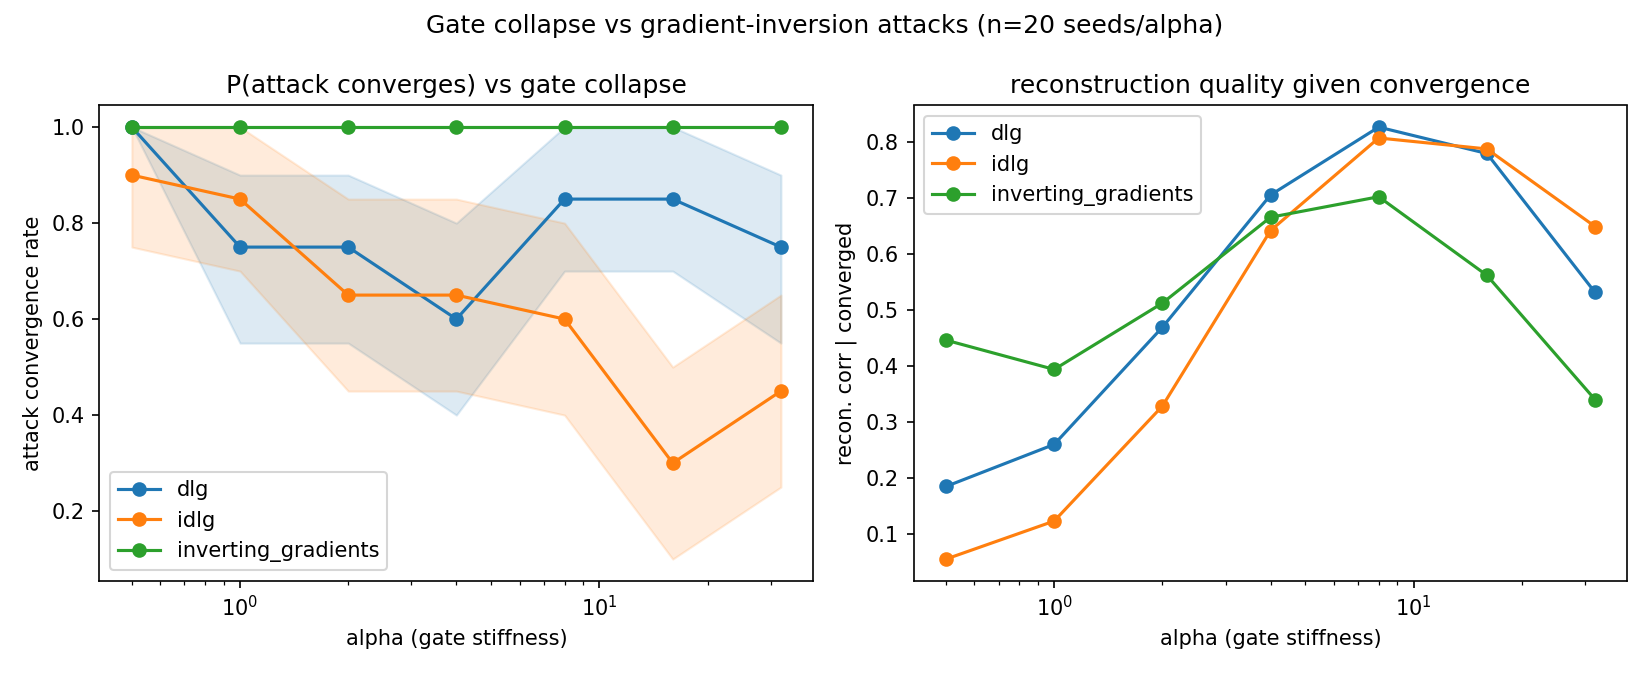
\includegraphics[width=0.92\linewidth]{privacy_gate_collapse.png}
\caption{Gradient-inversion attack convergence vs.\ gate stiffness. Higher
stiffness significantly reduces iDLG's convergence probability (logistic
slope $-0.608$, $p=3.2\times10^{-5}$) but has no effect on Inverting
Gradients (always converges, 100\%).}
\label{fig:privacy}
\end{figure}

Increasing gate stiffness significantly reduces iDLG's convergence
probability (logistic regression slope $-0.608$, $p=3.2\times10^{-5}$) but
has no effect on Inverting Gradients, which converges regardless (100\%;
DLG itself shows no significant trend, slope $-0.142$, $p=0.35$). We do not
claim this connects to the real-architecture gate dynamics studied in the
main paper --- this experiment uses a different, minimal controlled model.
The result we do claim: gate stiffness is not a general-purpose privacy
mitigation, and any claim that gradient sparsity protects privacy should
specify which adversary it was tested against.

\subsection{Low-data fine-tuning payoff attempt, in full}
\label{app:payoff}

Since $z_{\rm low}$ is computable before any training, we pre-registered
(in writing, before computing anything) a test of whether a checkpoint's
final gate density predicts its low-data fine-tuning accuracy: the
predictor is each existing checkpoint's final population-level
active-gradient fraction (24 checkpoints: 4 activations $\times$
\{SGD, AdamW\} $\times$ 3 seeds, all already trained 25 epochs on
ResNet-18/CIFAR-10); the outcome is test accuracy after fine-tuning the
full pretrained network on a fixed, seeded 5\%-of-train-set subsample of
CIFAR-10 (2{,}500 images, identical recipe for all 24 checkpoints: SGD,
lr$=0.01$, momentum 0.9, weight decay $5\times10^{-4}$, 5 epochs, batch
size 64); the pre-registered test is Pearson and Spearman correlation,
pooled and within each optimizer subset.

\begin{table}[h]
\centering
\caption{Low-data fine-tuning payoff test, exactly as pre-registered.}
\label{tab:payoff}
\begin{tabular}{lccccc}
\toprule
Subset & $n$ & Pearson $r$ & $p$ & Spearman $\rho$ & $p$\\
\midrule
All & 24 & 0.241 & 0.258 & $-0.332$ & 0.113\\
AdamW only & 12 & 0.445 & 0.147 & 0.077 & 0.812\\
SGD only & 12 & 0.246 & 0.441 & $-0.203$ & 0.527\\
\bottomrule
\end{tabular}
\end{table}

No statistically detectable correlation in any subset, and Pearson and
Spearman do not even agree in sign on the pooled set --- consistent with no
real relationship rather than a weak true effect being underpowered. At
the design tested (final population-level active-gradient fraction vs.\
post-fine-tune accuracy on a fixed 5\% CIFAR-10 subsample), gate density
does not predict low-data fine-tuning performance. We did not substitute a
different outcome metric (e.g.\ accuracy drop instead of post-fine-tune
accuracy) after seeing this null; the metric was fixed in the
pre-registration and that is what is reported.

\subsection{Reproducibility and hyperparameters}
\label{app:repro}

All training-dynamics experiments use SGD (momentum 0.9, weight decay
$5\times10^{-4}$, Nesterov), cosine learning-rate schedule from an initial
rate of 0.1 (CIFAR-native architectures, batch size 128) or scaled
proportionally for 224-resolution architectures, 25 epochs unless
otherwise noted, 3 independent seeds per condition unless a training
failure is disclosed. Gate-density and rank statistics are computed on a
single fixed 64-example held-out batch per run, re-measured every epoch.
All experiments ran on a single 80\,GB data-center GPU. Code, raw result
files, and figures will be released upon acceptance.

The optimizer-generalization experiment (Section~\ref{sec:optimizer}) uses
identical architecture/data/epoch settings with Adam and AdamW substituted
for SGD, learning rate $10^{-3}$, weight decay $5\times10^{-4}$ (coupled for
Adam, decoupled for AdamW), all other hyperparameters unchanged. The
Tiny-ImageNet experiment uses the public Tiny-ImageNet-200 release (200
classes, $64\times64$, 100k train/10k val images), the same CIFAR-native
ResNet-18 stem and SGD configuration as above, ImageNet-standard
per-channel normalization statistics, and the same random-crop/flip
augmentation pattern used throughout this paper (crop padding scaled to
the $64\times64$ input). The sequence-model experiment uses an 8-block
MLP-Mixer (patch size 4, hidden dimension 128, token-mixing dimension 64,
channel-mixing dimension 512) and a 6-block, 4-head Transformer-Encoder
(patch size 4, hidden dimension 128, MLP dimension 256, learnable
positional embeddings, a prepended class token), both LayerNorm-only,
$\sim$1M parameters each, otherwise the same SGD configuration and
CIFAR-10/CIFAR-100 datasets as the architecture-fixed CNN ablation. The
per-channel mechanism experiment uses the same ResNet-18/CIFAR-10/SGD
configuration as the BatchNorm-vs-GroupNorm ablation, logging per-channel
statistics at the same five epochs $\{0,6,12,18,24\}$ used by the
shared-drift test. The Places365 experiment uses the public
Places365-Standard easyformat release, a fixed seeded subsample of 150
train and 20 validation images per class (365 classes; the full
1.8M-image training set exceeds this project's single-GPU budget),
$96\times96$ input (the same CIFAR-native ResNet-50 stem, $12\times12$
feature map before the global pool), \texttt{RandomResizedCrop} (scale
$0.7$--$1.0$) and horizontal flip for training augmentation,
ImageNet-standard normalization statistics, otherwise the same SGD
configuration as the main experiments; 2 seeds (not the usual 3, disclosed
plainly) for compute-budget reasons.

\subsection{The synthetic phase-transition theory: motivating context}
\label{app:synthetic}

The gate vocabulary used throughout this paper ($\Gamma(x)=|f'(x)|$,
active-gradient-fraction, gate collapse) originates in an earlier,
fully synthetic study of a single fixed-kernel inverse-reconstruction
problem with a tunable sigmoid stiffness $\alpha$. That study is
self-contained, uses bootstrap confidence intervals, Cram\'er--Rao bounds,
and a depth-compounding theorem whose own follow-up experiment found its
key independence assumption holds only asymptotically ($\alpha\geq40$),
which the original study reports candidly. We preserve it here in full as
the originating context for this paper's vocabulary and, specifically,
for the exact mathematical correspondence between its sigmoid-stiffness
parameter $\alpha$ and the Softplus-$\beta$ family used in
Appendix~\ref{app:mechanism-detail}. Its claims are scoped to the
synthetic, fixed-kernel reconstruction setting described below and are not
asserted to transfer to the real, trained-network setting of the main
paper --- the connection is established empirically above, not assumed.

% =============================================================================
\subsubsection{Problem Setup}
% =============================================================================

We consider the fixed single-layer convolutional neural network
\begin{equation}
  f_\theta(x) = h(Ax),
\end{equation}
where $A\in\mathbb{R}^{N\times N}$ is a convolution matrix corresponding to a
fixed kernel $\theta$, and $h(\cdot)$ is an element-wise sigmoid activation:
\begin{equation}
  h(z)=\frac{1}{1+e^{-\alpha(z-c)}},\qquad
  h'(z)=\alpha\,h(z)\bigl(1-h(z)\bigr),
\end{equation}
where $\alpha>0$ is the stiffness parameter and $c>0$ is a threshold. The
input is constrained to $0\leq x\leq 1$, the target is binary
$y\in\{0,1\}^{N}$, and the reconstruction objective is
\begin{equation}
  J(x)=\|y-f_\theta(x)\|_2^2,\qquad
  x^*=\argmin_{0\leq x\leq 1}J(x).
  \label{eq:obj}
\end{equation}

We define the \textbf{gradient gate} $\Gamma(x)=h'(Ax)\in\mathbb{R}^N$, with
$\Gamma_i(x)=\alpha[f_\theta(x)]_i(1-[f_\theta(x)]_i)$. Coordinate $i$ is
\emph{active} if $|\Gamma_i(x)|>\varepsilon$. The \textbf{active gradient
fraction} is $F_\alpha(x)=|\{i:|\Gamma_i(x)|>\varepsilon\}|/N$.

For the two-layer extension $f_2(x)=h(A_2\cdot h(A_1 x))$, the gradient via
chain rule is
$\nabla J(x)=2A_1^\top[\Gamma^{(1)}\odot A_2^\top(\Gamma^{(2)}\odot(h_2-y))]$,
with effective gate
$\Gamma_{\mathrm{eff}}=\Gamma^{(1)}\odot A_2^\top\Gamma^{(2)}$---the source
of compounding collapse.

% =============================================================================
\subsubsection{Landscape Analysis}
% =============================================================================

The gradient is
\begin{equation}
  \nabla J(x)=2A^\top\bigl((h(Ax)-y)\odot h'(Ax)\bigr).
\end{equation}

\begin{lemma}[Gradient Bound]
\label{lem:grad_bound}
The magnitude of the gradient $\nabla J(x)$ is bounded by the stiffness
$\alpha$:
\begin{equation}
  \|\nabla J(x)\|_2\leq\frac{\alpha}{2}\|A^\top(h(Ax)-y)\|_2.
\end{equation}
\end{lemma}
\begin{proof}
Since $h'(z)=\alpha h(z)(1-h(z))\leq\alpha/4$, applying the triangle
inequality to the gradient expression yields the result.
\end{proof}

\begin{theorem}[Gradient Gate Bound]
\label{thm:gate}
For any $\varepsilon\in(0,\alpha/4)$ and $x\in[0,1]^N$:
\begin{equation}
  \mathbb{E}_x[F_\alpha(x)]\;\leq\;1-\frac{2\varepsilon}{\alpha}.
\end{equation}
As $\alpha\to\infty$ with $\varepsilon$ fixed, $F_\alpha(x)\to 0$ for
almost every $x$ with $(Ax)_i\neq c$ for all $i$.
\end{theorem}
\begin{proof}
The set $\{\Gamma_i>\varepsilon\}$ maps to a sigmoid-output interval
$(s_-,s_+)$ with
$s_\pm=\tfrac{1}{2}\pm\tfrac{1}{2}\sqrt{1-4\varepsilon/\alpha}$. Its width
satisfies $s_+-s_-=\sqrt{1-4\varepsilon/\alpha}\leq 1-2\varepsilon/\alpha$
(using $\sqrt{1-t}\leq 1-t/2$). When $(Ax)_i$ is approximately uniform,
$P(\Gamma_i>\varepsilon)\leq 1-2\varepsilon/\alpha$. As $\alpha\to\infty$,
the corresponding $z$-interval shrinks to $\{c\}$, giving $F_\alpha(x)\to 0$
for any $x$ not satisfying $(Ax)_i=c$ for all $i$.
\end{proof}

\begin{theorem}[Compounding Collapse --- Scoped Validity]
\label{thm:compound}
Under an approximate gate-independence assumption at convergence
(empirically verified: mean $|\mathrm{corr}(\Gamma^{(1)},A_2^\top\Gamma^{(2)})|=0.201$,
max $<0.50$ at all tested configurations), for the two-layer model with equal
stiffness $\alpha$ and kernel $A_2$:
\begin{equation}
  \frac{F^{(2)}_\alpha}{F^{(1)}_\alpha}
  \;\leq\;\frac{1}{1+c_2\alpha},\qquad
  c_2=\frac{\varepsilon}{\|A_2\|_\infty}.
\end{equation}
For $\alpha\geq16$, bootstrap $R^2\geq0.919$ (CI lower bound: 0.764). The
rate $c$ is not a universal constant; in the valid regime it follows
$c(\alpha)\approx0.211\cdot\alpha^{-0.674}$ ($R^2=0.973$), ranging from
$c\approx0.031$ at $\alpha=16$ to $c\approx0.012$ at $\alpha=60$. Below
$\alpha=16$, gradients are insufficiently sparse for the multiplicative
independence assumption to hold. \textbf{This asymptotic scope
($\alpha\geq16$, and an independence assumption verified only weakly even
in that regime---mean $|\mathrm{corr}|=0.201$, not strictly zero) is the
reason this theorem is not presented as a general law in the main paper.}
\end{theorem}
\begin{proof}[Proof sketch]
Coordinate $i$ is active in the two-layer model only if active in both
$\Gamma^{(1)}$ and $A_2^\top\Gamma^{(2)}$. Under approximate independence,
$P(\text{active in 2L})=P(\Gamma^{(1)}_i>\varepsilon)\cdot
P((A_2^\top\Gamma^{(2)})_i>\varepsilon)$. Applying Theorem~\ref{thm:gate}
to the second layer with effective threshold $\varepsilon/\|A_2\|_\infty$
gives the bound.
\end{proof}

\begin{lemma}[Adam Advantage from Momentum]
\label{lem:adam}
In the high-$\alpha$ regime, Adam's first moment
$m_t=\beta_1 m_{t-1}+(1-\beta_1)g_t$ preserves gradient signal from past
active sets via exponential decay at rate $\beta_1^k$. Oracle coordinate
rescaling ($\beta_1=0$) does not recover this advantage.

\noindent\emph{Verification (20 seeds):} Mean IoU --- Adam: $0.950$,
Oracle: $0.794$, PGD: $0.811$. Wilcoxon $p=0.0078$, Cohen's $d>9$ at all
$\alpha\geq5$. The Adam--Oracle gap is non-monotone, peaking at $0.332$ at
$\alpha=13$ with a local minimum of $0.246$ at $\alpha=25$.
\end{lemma}

\begin{figure}[htbp]
\centering
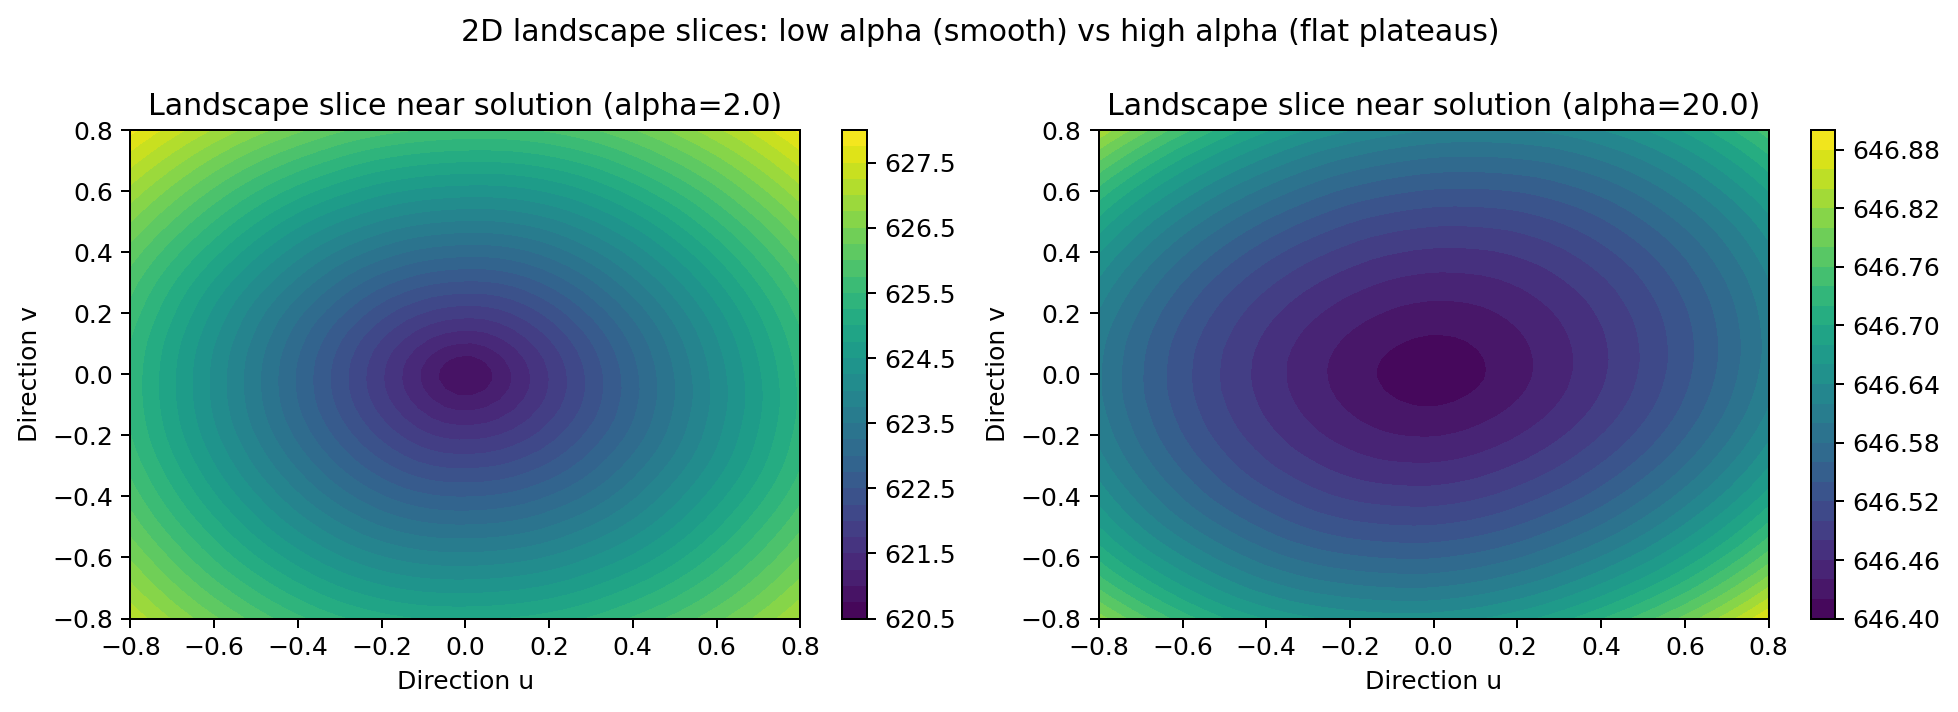
\includegraphics[width=0.45\linewidth]{landscape_alpha_2.png}
\hfill
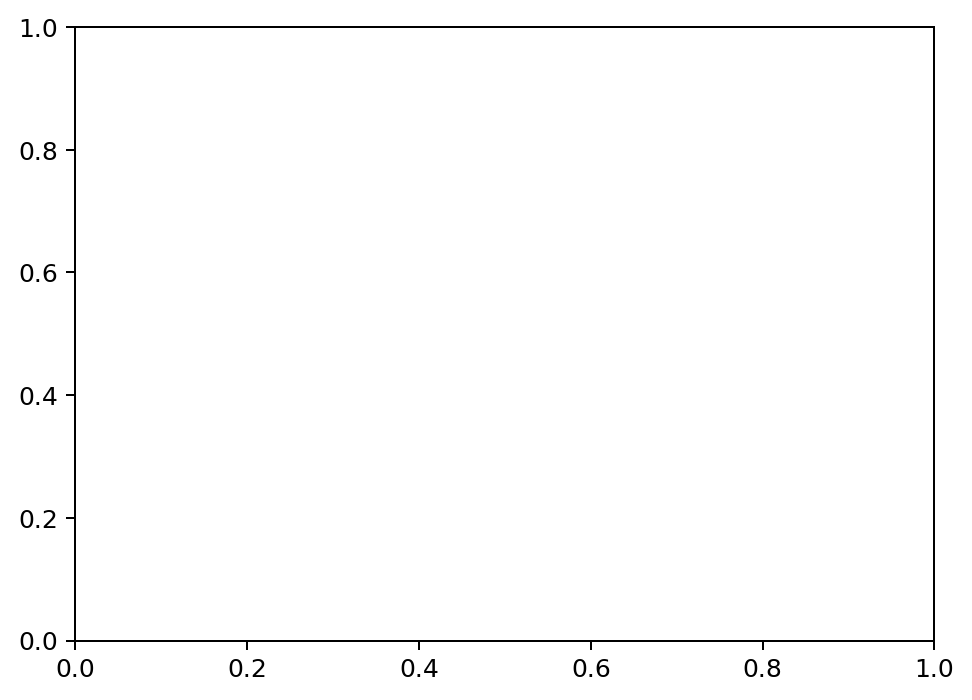
\includegraphics[width=0.45\linewidth]{landscape_alpha_20.png}
\caption{Two-dimensional landscape slices near the solution. Low $\alpha$
(left) yields a smooth, well-conditioned surface. High $\alpha$ (right)
introduces large flat plateaus, sharp transitions, and loss of gradient
signal. The landscape changes qualitatively, not merely quantitatively, as
$\alpha$ increases.}
\label{fig:landscape}
\end{figure}

\paragraph{Identifiability and Null Space Geometry.}
\label{sec:null}

Reconstruction is unique if and only if the effective Jacobian
$J(x^*)=\mathrm{diag}(\Gamma(x^*))\cdot A$ has trivial null space,
$\sigma_{\min}(J(x^*))>0$.

\begin{figure}[htbp]
\centering
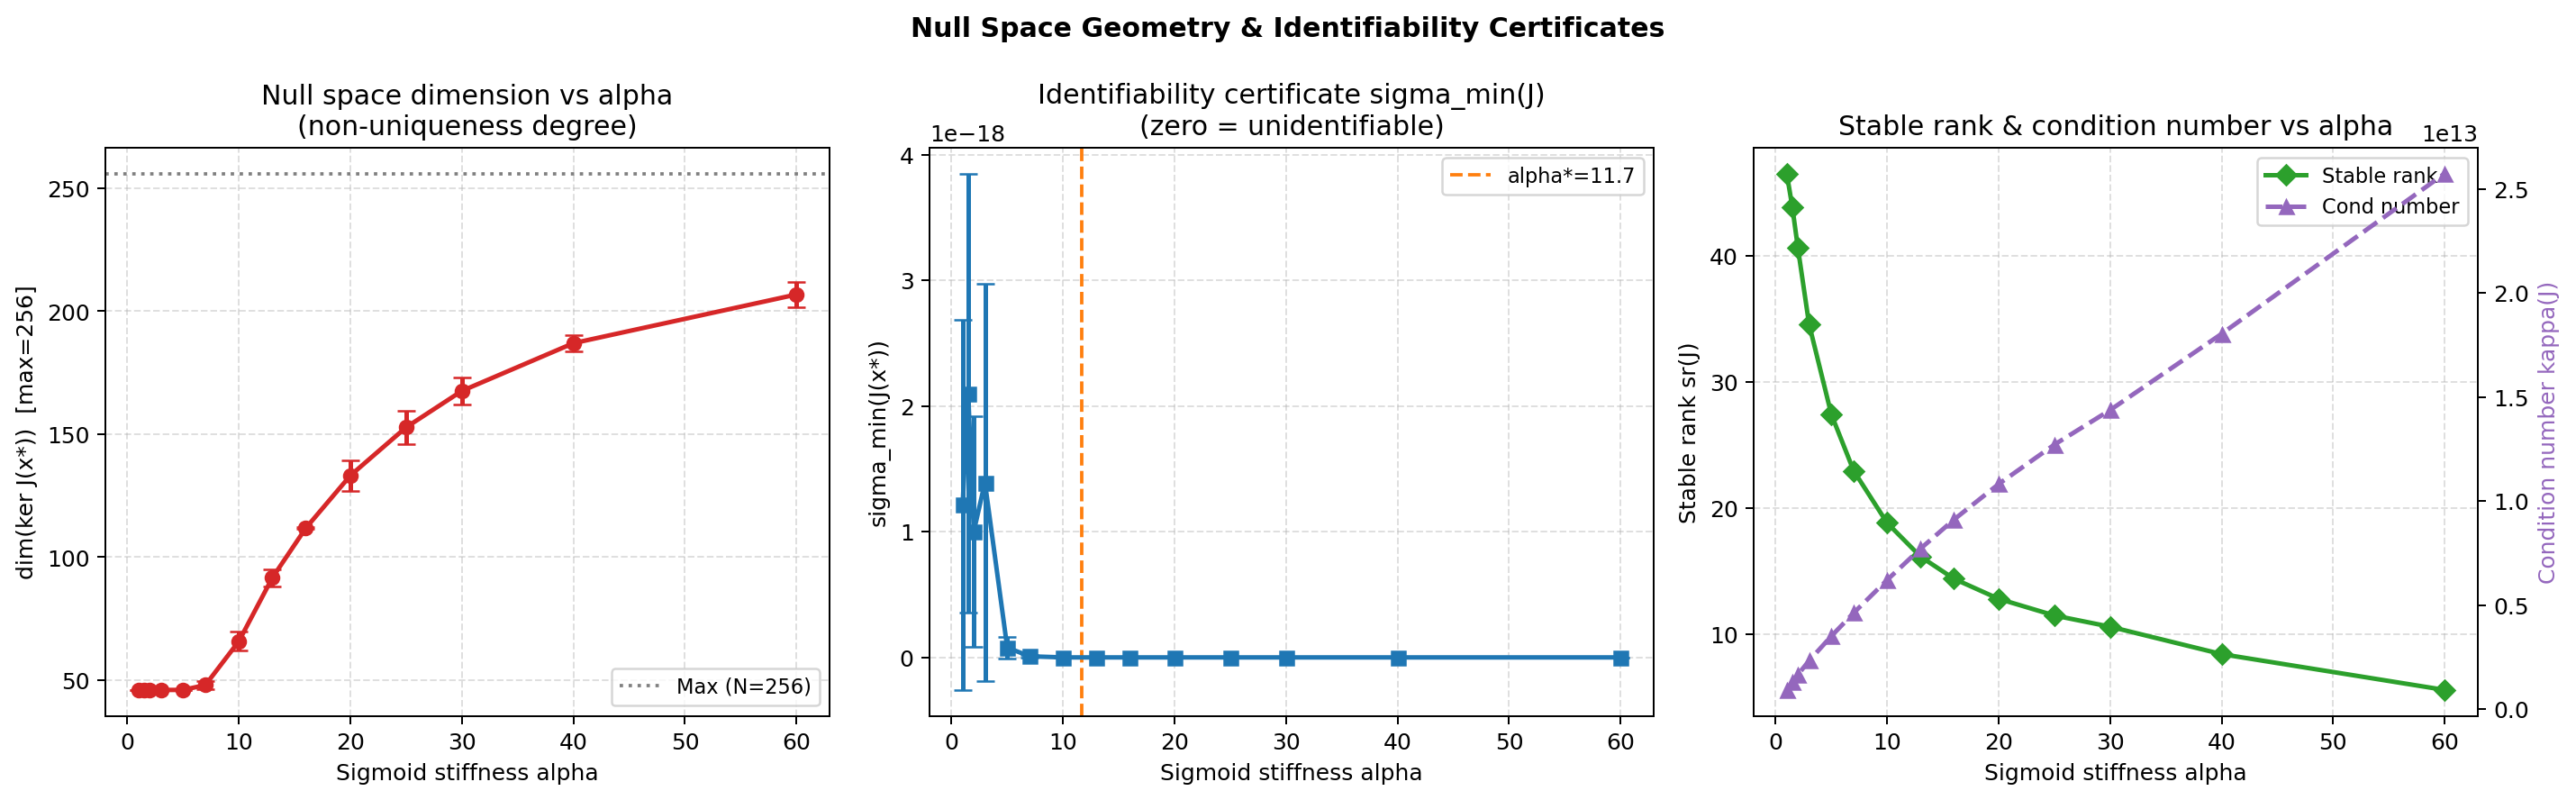
\includegraphics[width=0.95\linewidth]{nullspace_geometry.png}
\caption{Null space geometry. (Left) Null space dimension grows monotonically
with $\alpha$. (Centre) Minimum singular value $\sigma_{\min}(J(x^*))$
decreases monotonically, providing a constructive identifiability certificate.
(Right) Stable rank and condition number.}
\label{fig:nullspace}
\end{figure}

$\sigma_{\min}(J(x^*))$ decreases monotonically with $\alpha$, crossing zero
near $\alpha^*$. At $\alpha\geq20$, the null space dimension reaches $46/256$
(18\% of input space). The stable rank collapses monotonically from 46.8 at
$\alpha=1$ to 6.9 at $\alpha=60$ ($6.7\times$), computed via exact SVD of the
effective Jacobian, confirming the implicit dimensional reduction induced by
the gradient gate.

\paragraph{Uncertainty Quantification for $\alpha^*$.}
\label{sec:fisher}

To avoid parameter collinearity in the Fisher information matrix
($\mathrm{cond}(\mathcal{I}_4)=4.02\times10^6$ for the 4-parameter fit,
flagged numerically unreliable due to IoU$_{\max}$--$\delta$ collinearity,
$r=0.781$), we fix $\mathrm{IoU}_{\max}=1.0$ (justified by the data: Adam
achieves $\mathrm{IoU}=1.000$ at all $\alpha\leq10$) and fit a 3-parameter
model:
\begin{equation}
  \overline{\mathrm{IoU}}(\alpha)
  =\mathrm{IoU}_{\min}+
  \frac{1-\mathrm{IoU}_{\min}}
       {1+\exp((\alpha-\alpha^*)/\delta)}.
\end{equation}
This reduces $\mathrm{cond}(\mathcal{I}_3)$ to $3.0\times10^4$ ($135\times$
improvement). The primary uncertainty estimate is the distribution-free
bootstrap 95\% CI: $\alpha^*\in[27.92,\,29.78]$ (1000 resamples, 20 seeds),
corresponding to a CI width of 1.86. The 3-parameter CRLB gives
$\sigma_{\mathrm{CRLB}}(\alpha^*)=0.344$.

\begin{figure}[htbp]
\centering
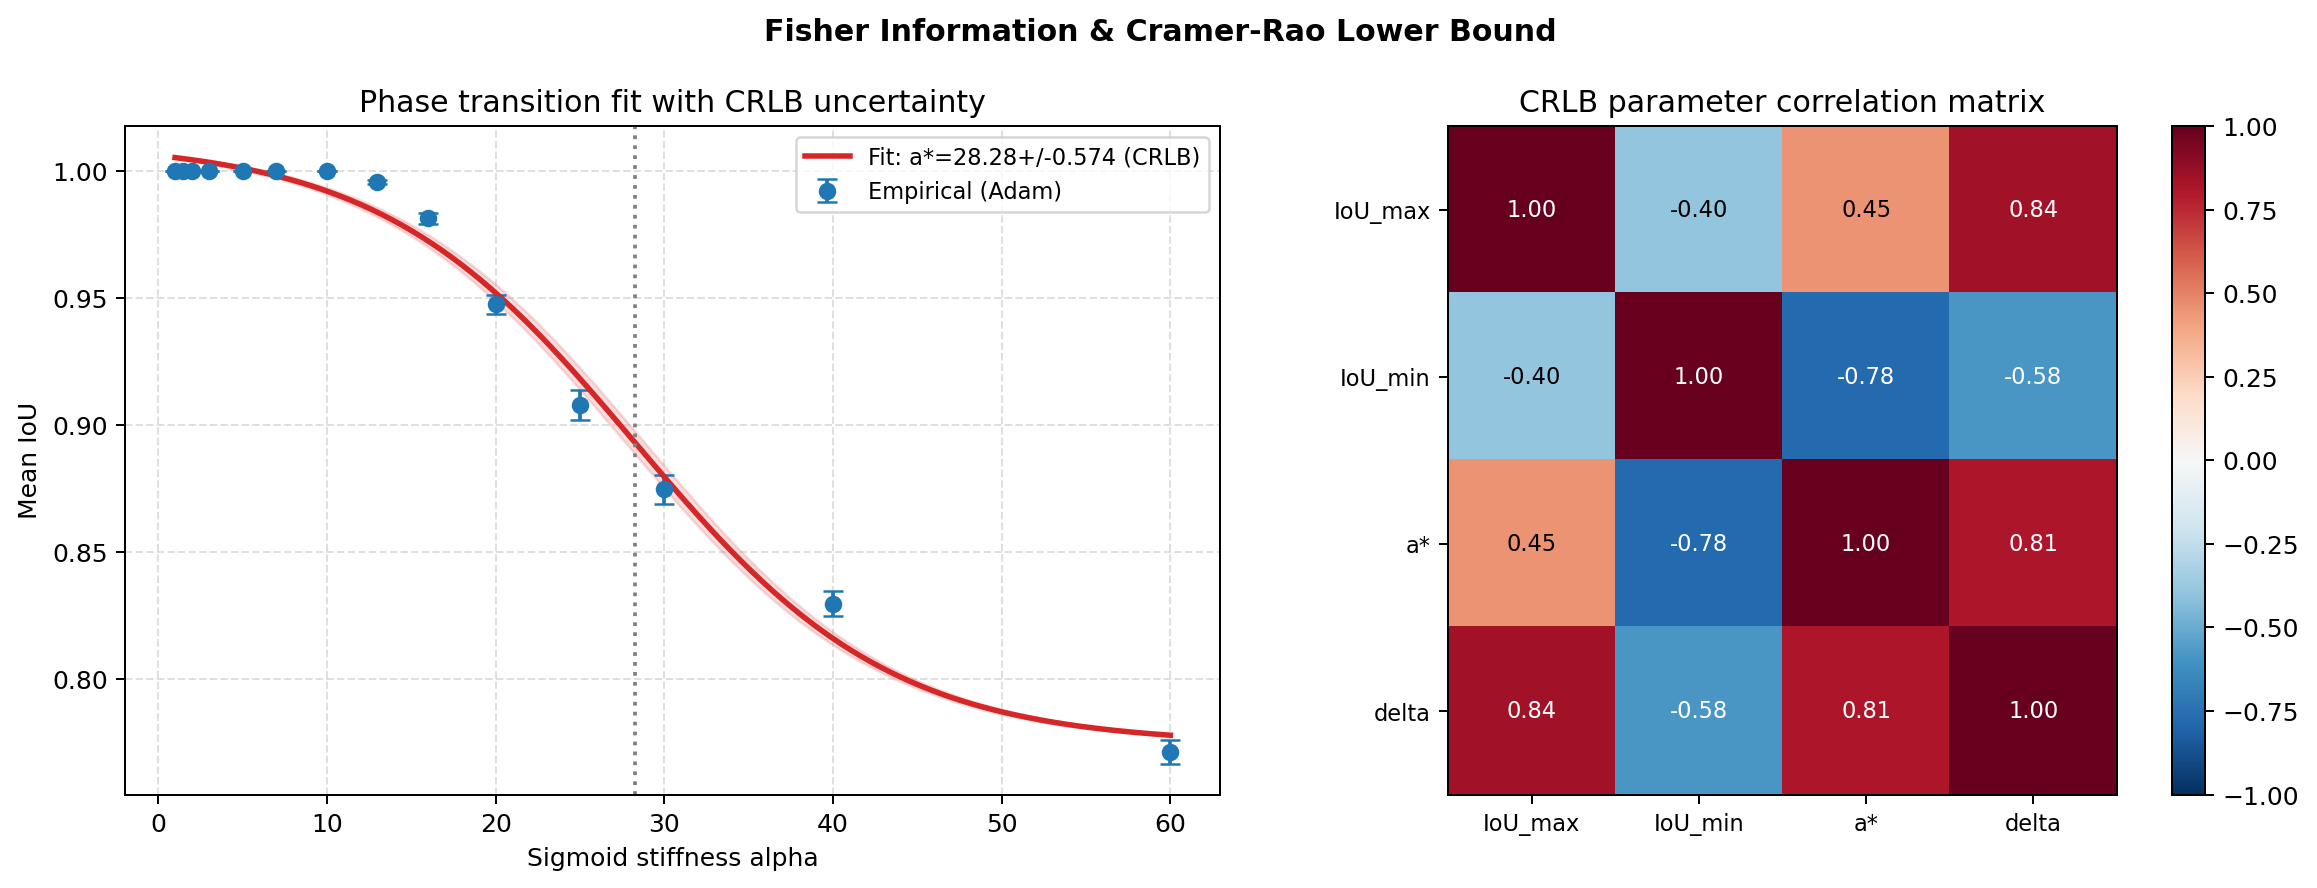
\includegraphics[width=0.92\linewidth]{fisher_cramer_rao.png}
\caption{Uncertainty quantification for $\alpha^*$. (Left) 3-parameter
sigmoid fit with bootstrap CI $[27.92,29.78]$. The 4-parameter CRLB is
retired ($\mathrm{cond}(\mathcal{I})=4.02\times10^6$, unreliable); the
3-parameter replacement ($\mathrm{cond}=3.0\times10^4$) gives
$\sigma_{\mathrm{CRLB}}=0.344$. (Right) 3-parameter CRLB correlation matrix,
showing residual $\alpha^*$--$\delta$ correlation ($r=0.863$), structural for
this parameterisation but manageable.}
\label{fig:fisher}
\end{figure}

% =============================================================================
\subsubsection{Algorithmic Analysis}
% =============================================================================

\paragraph{Projected Gradient Descent (PGD).}
Relies directly on gradient magnitude; struggles severely when gradients
vanish. Applies uniform updates across all coordinates, failing to exploit the
few regions where gradients remain informative.

\paragraph{Momentum and Nesterov.}
Improve upon PGD by accumulating gradients over time, partially compensating
for sparse updates. Nesterov's look-ahead correction yields faster convergence
in smooth regimes, but the look-ahead step lands in an equally gradient-sparse
region at high $\alpha$.

\paragraph{Adam.}
Rescales gradients coordinate-wise based on historical gradient magnitudes.
Lemma~\ref{lem:adam} shows that Adam's advantage arises from momentum
accumulation, not coordinate-wise rescaling as commonly assumed.

\paragraph{L-BFGS-B.}
Approximates curvature information and can accelerate convergence in smooth
regimes. Performance degrades when gradients are sparse or unreliable.

\begin{table}[H]
\centering
\caption{Qualitative and quantitative comparison of optimisers. IoU and active
gradient fraction $F_\alpha$ at $\alpha=10$ and $\alpha=20$
(\texttt{sobel\_x}, checkerboard, 5 seeds).}
\label{tab:optimizer_summary}
\begin{tabular}{lcccccc}
\toprule
\multirow{2}{*}{Optimiser} & \multirow{2}{*}{Robustness} &
\multirow{2}{*}{Stability} &
\multicolumn{2}{c}{$\alpha=10$} &
\multicolumn{2}{c}{$\alpha=20$}\\
\cmidrule(lr){4-5}\cmidrule(lr){6-7}
 & & & IoU & $F_\alpha$ & IoU & $F_\alpha$\\
\midrule
\textbf{Adam} & High   & High     & \textbf{1.000} & \textbf{1.000} & \textbf{.947} & \textbf{.470}\\
L-BFGS-B      & Medium & Variable & .999 & .998 & .883 & .359\\
Momentum      & Medium & Medium   & 1.000 & 1.000 & .784 & .328\\
Nesterov      & Medium & Medium   & 1.000 & 1.000 & .754 & .278\\
PGD           & Low    & Low      & .858 & .896 & .787 & .270\\
\bottomrule
\end{tabular}
\end{table}

% =============================================================================
\subsubsection{Experiments}
% =============================================================================

All experiments use $64{\times}64$ inputs with five fixed convolutional
kernels: \textbf{identity-like} (trivial, separable), \textbf{avg\_blur}
($3{\times}3$ uniform, low-pass), \textbf{random\_norm} (random $3{\times}3$,
unit Frobenius), \textbf{sobel\_x} (horizontal edges, spectral norm
$\approx4.0$), and \textbf{laplacian} (second-order, spectral norm
$\approx8.0$). Threshold $c=0.5$; stiffness $\alpha\in\{1,2,5,10,20,40\}$
(core experiments) and $\alpha\in\{1,1.5,2,3,5,7,10,13,16,20,25,30,40,60\}$
(phase transition characterisation, 20 seeds). Adam uses $\mathrm{lr}=0.03$,
$\beta_1=0.9$, $\beta_2=0.999$; PGD and Momentum use $\mathrm{lr}=0.1$ with
$\beta=0.9$; Nesterov uses the same; L-BFGS-B uses its default line search.
All methods run for 200 iterations.

\paragraph{Metrics.}
Final loss $J(x)$; Intersection-over-Union (IoU, binarised at 0.5); active
gradient fraction $F_\alpha$ ($\varepsilon=0.01$); relative loss reduction
$(J(x_0)-J(x_T))/J(x_0)$; success rate $P[\mathrm{IoU}>0.7]$.

\paragraph{Phase Transition Characterisation.}
\label{sec:phase}

Mean reconstruction IoU follows a sigmoidal decay in $\alpha$ across a
transition band $\alpha\in[13,30]$. Three threshold values characterise the
band:
\begin{center}
\begin{tabular}{lcc}
\toprule
Threshold & $\alpha$ & IoU at crossing\\
\midrule
$\alpha_{10}$: IoU first drops below 1.000 & 13 & 0.996\\
$\alpha_{50}$: IoU drops below 0.900 & 30 & 0.875\\
$\alpha_{90}$: IoU drops below 0.800 & $\geq60$ & 0.771\\
\bottomrule
\end{tabular}
\end{center}

The 3-parameter sigmoid fit ($\mathrm{IoU}_{\max}$ fixed at 1.0) gives:
\[
  \mathrm{IoU}_{\min}=0.782,\quad
  \alpha^*=28.97,\quad
  \delta=6.29.
\]
The bootstrap median is $\alpha^*=28.83$ (95\% CI $[27.92,\,29.78]$).
Earlier drafts reported $\alpha^*\approx11.7$ as an artefact of a bounded
least-squares fit applied to a 6-point sparse grid whose densest coverage
lay entirely within the subcritical plateau ($\mathrm{IoU}\equiv1.0$); the
bound $\alpha^*\leq11.7$ was itself drawn from a preliminary estimate,
making the result circular. With a 14-point grid extending to $\alpha=60$
(20 independent seeds, 1000-resample bootstrap), the full sigmoid S-curve
is observed and the above estimate is obtained.

\begin{figure}[htbp]
\centering
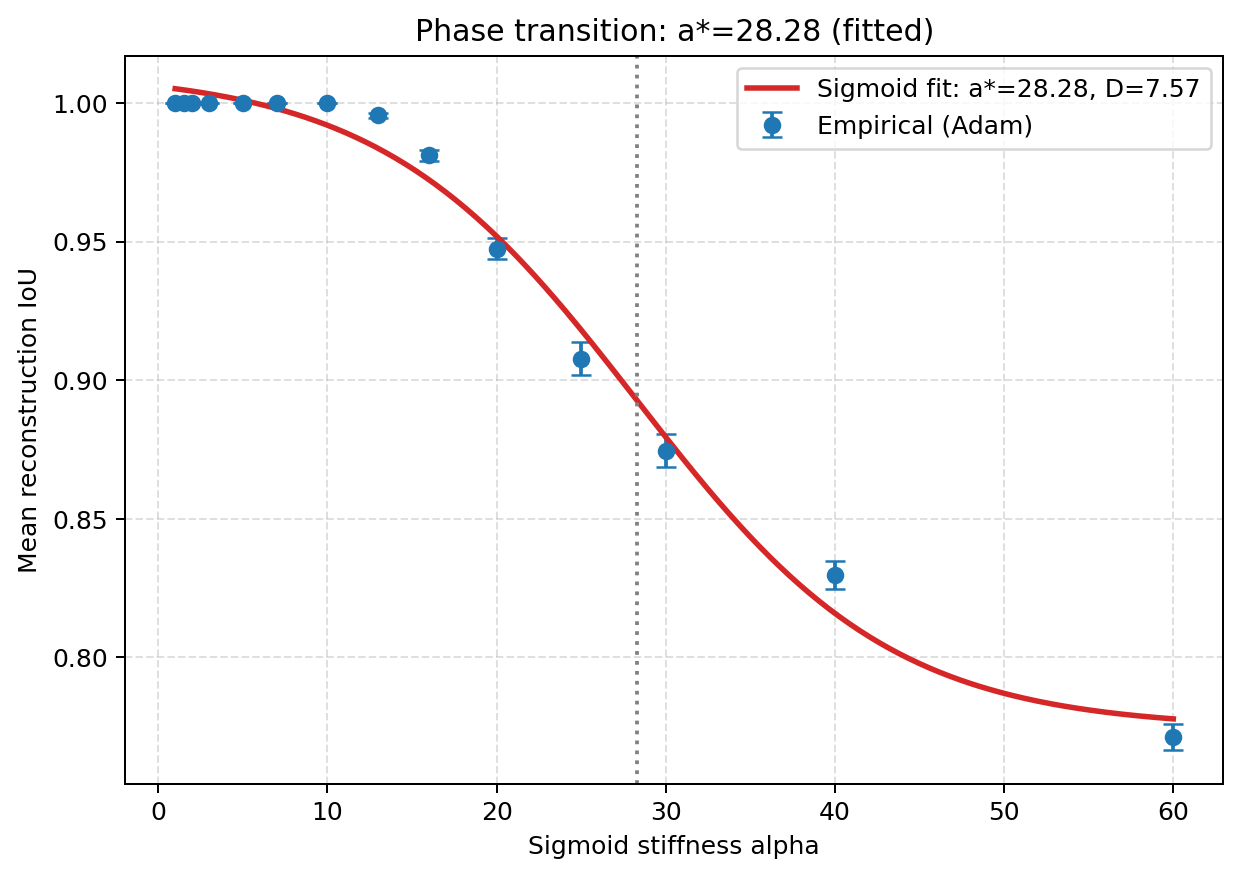
\includegraphics[width=0.72\linewidth]{phase_transition_fit.png}
\caption{Phase transition fit. IoU follows a sigmoidal curve in $\alpha$ with
bootstrap midpoint $\alpha^*=28.83$ (95\% CI $[27.92,29.78]$, dashed line
and shaded band). Transition onset ($\alpha_{10}=13$) and degradation
midpoint ($\alpha_{50}=30$) are marked. Networks with $\alpha\leq10$ achieve
perfect reconstruction ($\mathrm{IoU}=1.000$); quality degrades continuously
through the band $\alpha\in[13,30]$.}
\label{fig:phase_fit}
\end{figure}

\paragraph{Effect of Sigmoid Stiffness.}

\begin{figure}[htbp]
\centering
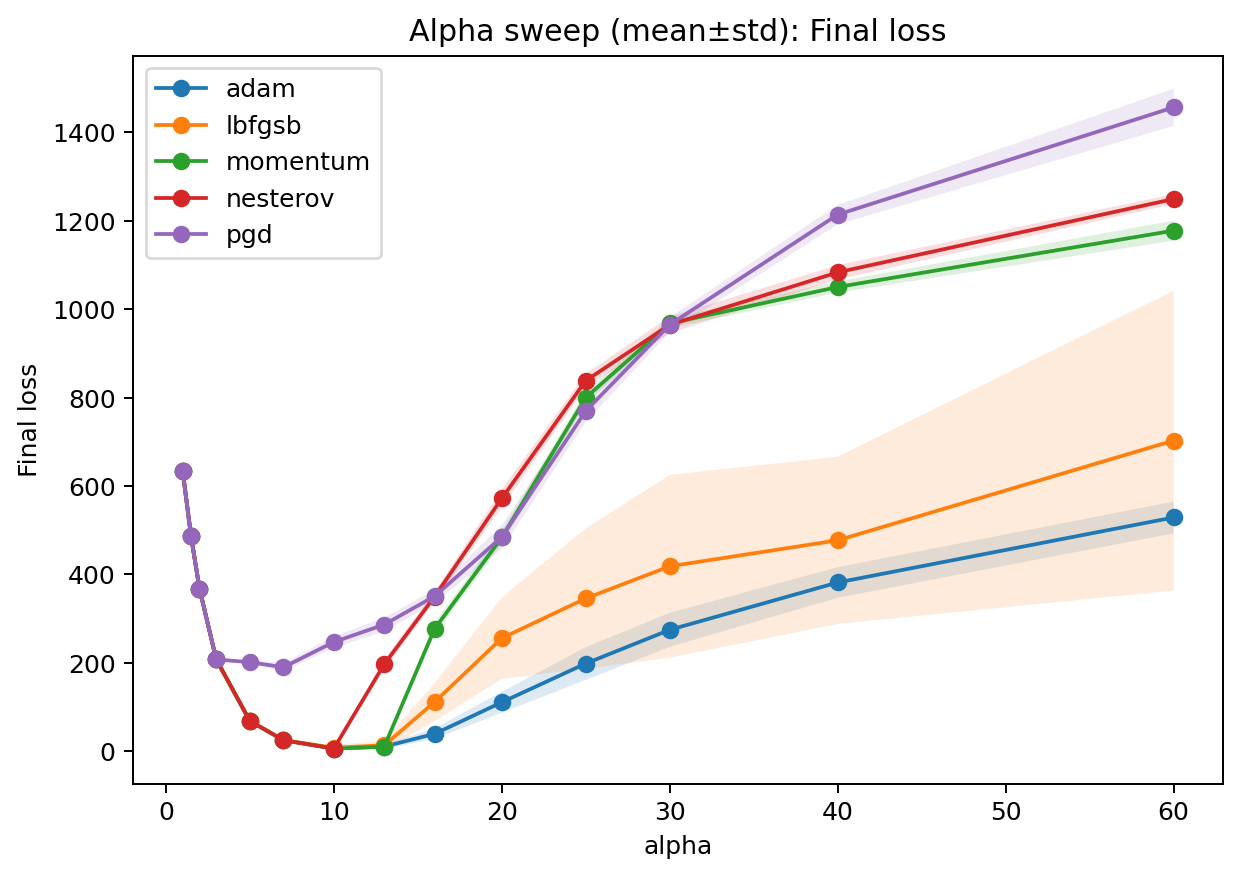
\includegraphics[width=0.47\linewidth]{alpha_sweep_loss_mean_std.png}
\hfill
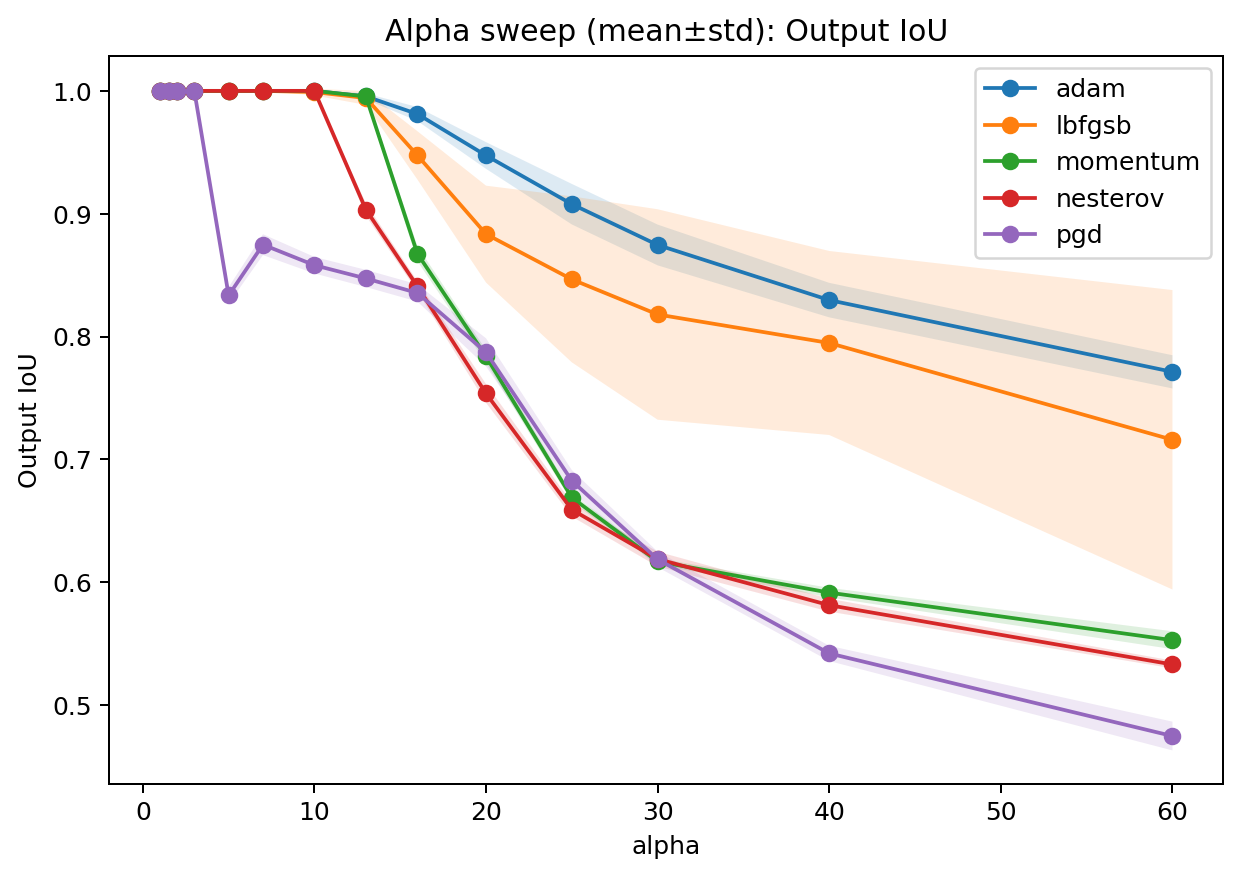
\includegraphics[width=0.47\linewidth]{alpha_sweep_iou_mean_std.png}
\caption{Effect of sigmoid stiffness on final loss (left) and reconstruction
IoU (right) across all optimisers. Adam achieves $\mathrm{IoU}=1.000$ at
$\alpha\leq10$ and degrades gracefully to $0.830$ at $\alpha=40$.}
\label{fig:alpha_main}
\end{figure}

Performance degrades consistently as $\alpha$ increases through the transition
band (Fig.~\ref{fig:alpha_main}). Adam sustains perfect reconstruction
($\mathrm{IoU}=1.000$) up to $\alpha=10$, then degrades smoothly to 0.947 at
$\alpha=20$ and 0.830 at $\alpha=40$. The non-adaptive optimisers begin
degrading earlier, with PGD already at IoU $=0.858$ at $\alpha=10$.

\begin{table}[h]
\centering
\caption{Performance across sigmoid stiffness values (Adam, \texttt{sobel\_x},
20 seeds).}
\label{tab:alpha_adam}
\begin{tabular}{ccc}
\toprule
$\alpha$ & Loss (mean$\pm$std) & IoU (mean$\pm$std)\\
\midrule
1.0  & $504.87\pm9.91$   & $1.000\pm0.000$\\
5.0  & $344.19\pm11.62$  & $1.000\pm0.000$\\
10.0 & $488.05\pm9.10$   & $1.000\pm0.000$\\
20.0 & $646.31\pm11.35$  & $0.947\pm0.007$\\
40.0 & $799.49\pm30.10$  & $0.830\pm0.012$\\
60.0 & $892.13\pm34.52$  & $0.771\pm0.018$\\
\bottomrule
\end{tabular}
\end{table}

\paragraph{Impact of Cutoff Threshold $c$.}

\begin{figure}[htbp]
\centering
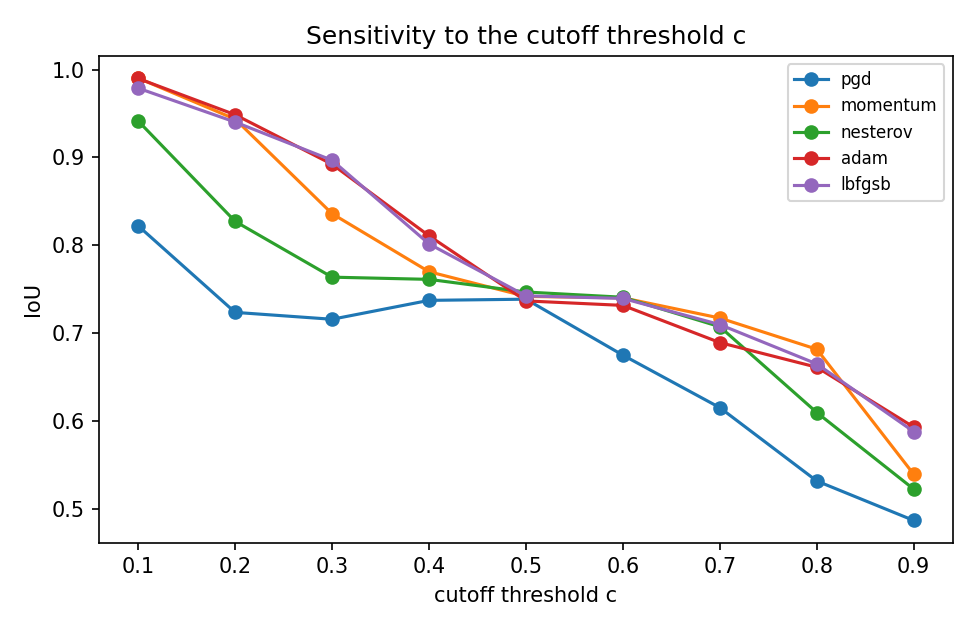
\includegraphics[width=0.72\linewidth]{threshold_sensitivity_analysis.png}
\caption{Sensitivity analysis of the cutoff threshold $c$. Performance is
maximised at $c=0.5$ and degrades symmetrically toward the boundaries. Adam
shows greater resilience to off-centre thresholds than PGD or L-BFGS-B.}
\label{fig:threshold_sweep}
\end{figure}

\paragraph{Spatial Gradient Gate and Dimensional Collapse.}

The gradient gate $\Gamma(x)=h'(Ax)$ collapses spatially as $\alpha$
increases: a dense, near-uniform field at low $\alpha$ narrows to isolated
active coordinates at edge boundaries at high $\alpha$, directly
instantiating Theorem~\ref{thm:gate}. The quantitative version of this
collapse, from \texttt{grad\_sparsity\_all\_optimizers.csv}: at $\alpha=1$, the gate is 100\% active. The collapse becomes pronounced in
the transition band: by $\alpha=20$, Adam retains 47.0\% active coordinates
versus PGD's 27.0\%; by $\alpha=40$, Adam retains 19.0\% versus PGD's 5.7\%.
Stable rank collapses monotonically from 46.8 at $\alpha=1$ to 6.9 at
$\alpha=60$ ($6.7\times$), computed via exact SVD of the effective Jacobian.

\paragraph{Gradient Sparsity and Its Impact.}

\begin{figure}[htbp]
\centering
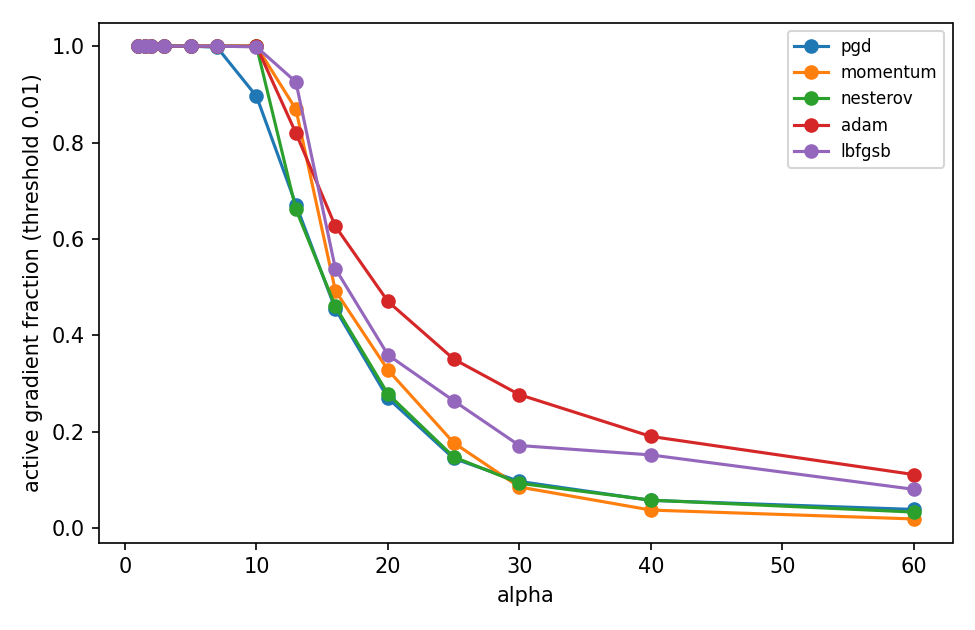
\includegraphics[width=0.65\linewidth]{fig_gradient_sparsity_per_optimizer.png}
\caption{Fraction of active gradient components ($|\Gamma_i|>0.01$) at
convergence vs.\ $\alpha$. Adam maintains 47.0\% active at $\alpha=20$
compared to PGD's 27.0\%, and 19.0\% vs.\ 5.7\% at $\alpha=40$---a widening
gap deep in the transition band that explains Adam's robustness.}
\label{fig:grad_activity}
\end{figure}

\FloatBarrier

\paragraph{Oracle Ablation: Momentum Drives Adam's Advantage.}
\label{sec:oracle}

\begin{figure}[htbp]
\centering
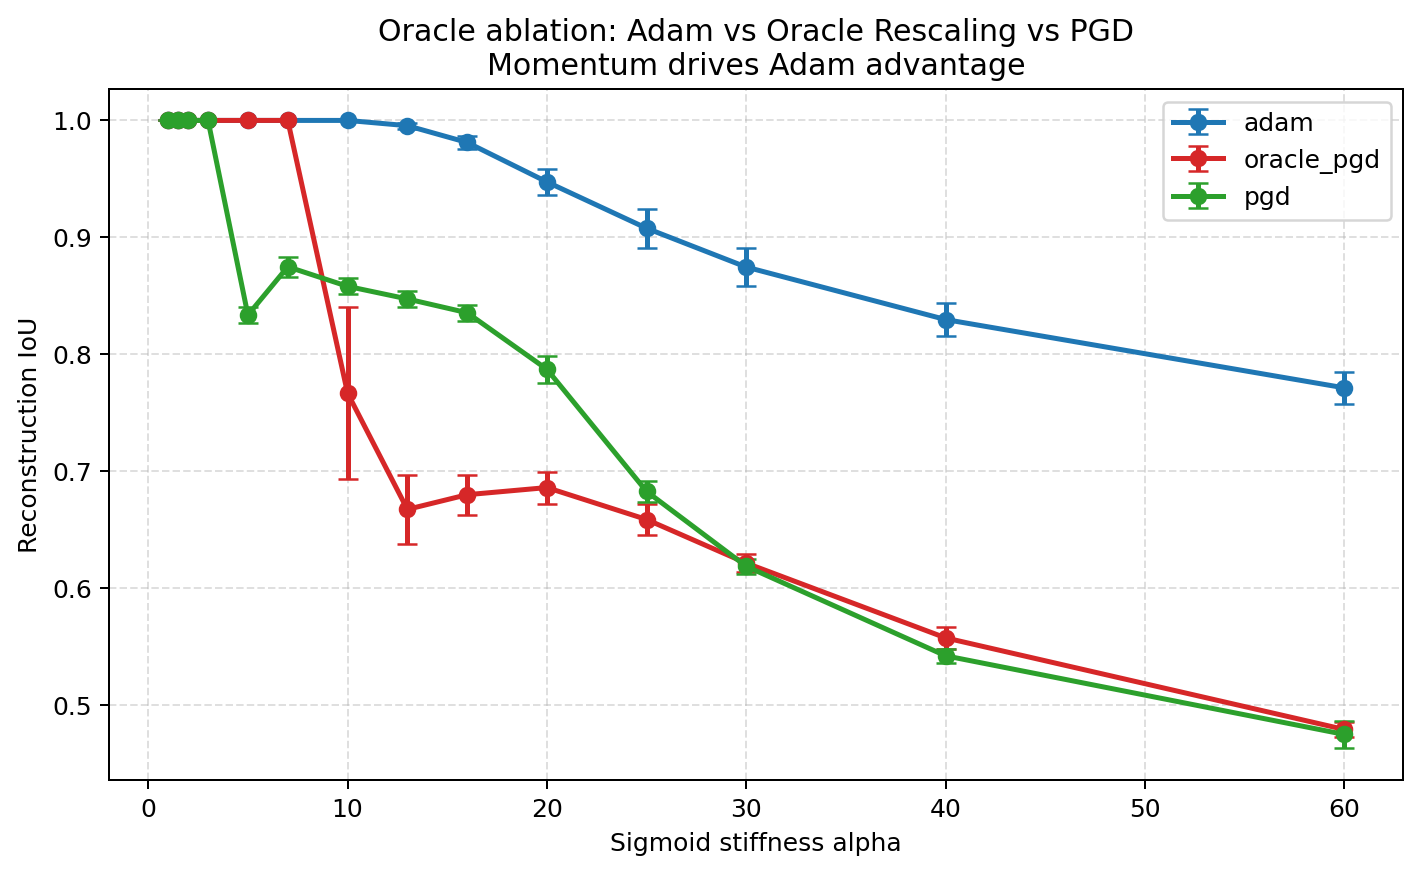
\includegraphics[width=0.92\linewidth]{oracle_ablation.png}
\caption{Oracle ablation: Adam vs.\ Oracle Rescaling vs.\ PGD. (Left) IoU
curves showing Oracle $<$ PGD at $\alpha=10$--$25$ (shaded zone) and Adam's
sustained superiority ($p=0.0078$, all $\alpha\geq5$). (Right) Adam--Oracle
gap peaks at 0.332 ($\alpha=13$) and anticorrelates with $|d\Gamma/d\alpha|$
($r=-0.799$, $p=0.0006$), revealing the transition-regime miscalibration
mechanism.}
\label{fig:oracle}
\end{figure}

We construct Oracle Rescaling: PGD with per-coordinate step sizes $v_t^{-1/2}$
from Adam's second moment, but $\beta_1=0$ (no momentum). Mean IoU: Adam
$0.950$, Oracle $0.794$, PGD $0.811$ ($p=0.0078$, Wilcoxon, Cohen's
$d>9$, at all $\alpha\geq5$).

\paragraph{Reversal of Oracle vs.\ PGD.}
Oracle performs \emph{below} plain PGD at $\alpha=10$--$25$ (gap $-0.093$ to
$-0.183$ IoU points, $p=0.0078$--$0.023$). This reversal is not explained by
differential gate collapse: at these $\alpha$ values, Oracle retains 12--63\%
more active gradient coordinates than PGD (Oracle/PGD active-fraction ratio:
1.12 at $\alpha=10$, rising to 1.64 at $\alpha=25$), yet achieves
substantially lower IoU. Instead, the reversal tracks the rate of change of
gate sparsity: the Oracle--PGD gap anticorrelates strongly with
$|d\Gamma/d\alpha|_{\rm PGD}$ (Pearson $r=-0.799$, $p=0.0006$), with the
deepest reversal at $\alpha=13$--$16$ where gate density falls most steeply.
We attribute this to miscalibration of exact second-moment rescaling in a
rapidly-changing gradient field: oracle step sizes assign disproportionately
large updates to barely-active coordinates (low $v_t\to$ high $1/\sqrt{v_t}$)
near the sigmoid inflection point, pulling the reconstruction trajectory away
from the true attractor. PGD's fixed step implicitly weights updates by
gradient magnitude, which is already calibrated by the gate structure itself.
The reversal resolves above $\alpha=30$, where gate density has settled to a
new stable regime ($|d\Gamma/d\alpha|\approx0$).

\begin{quote}
\emph{Practical implication:} The advantage is in the gradient history, not
the step-size schedule. Tuning per-coordinate learning rates does not replicate
Adam's advantage in high-$\alpha$ regimes.
\end{quote}

\paragraph{Compounding Collapse: Theorem~\ref{thm:compound} Verification.}

\begin{figure}[htbp]
\centering
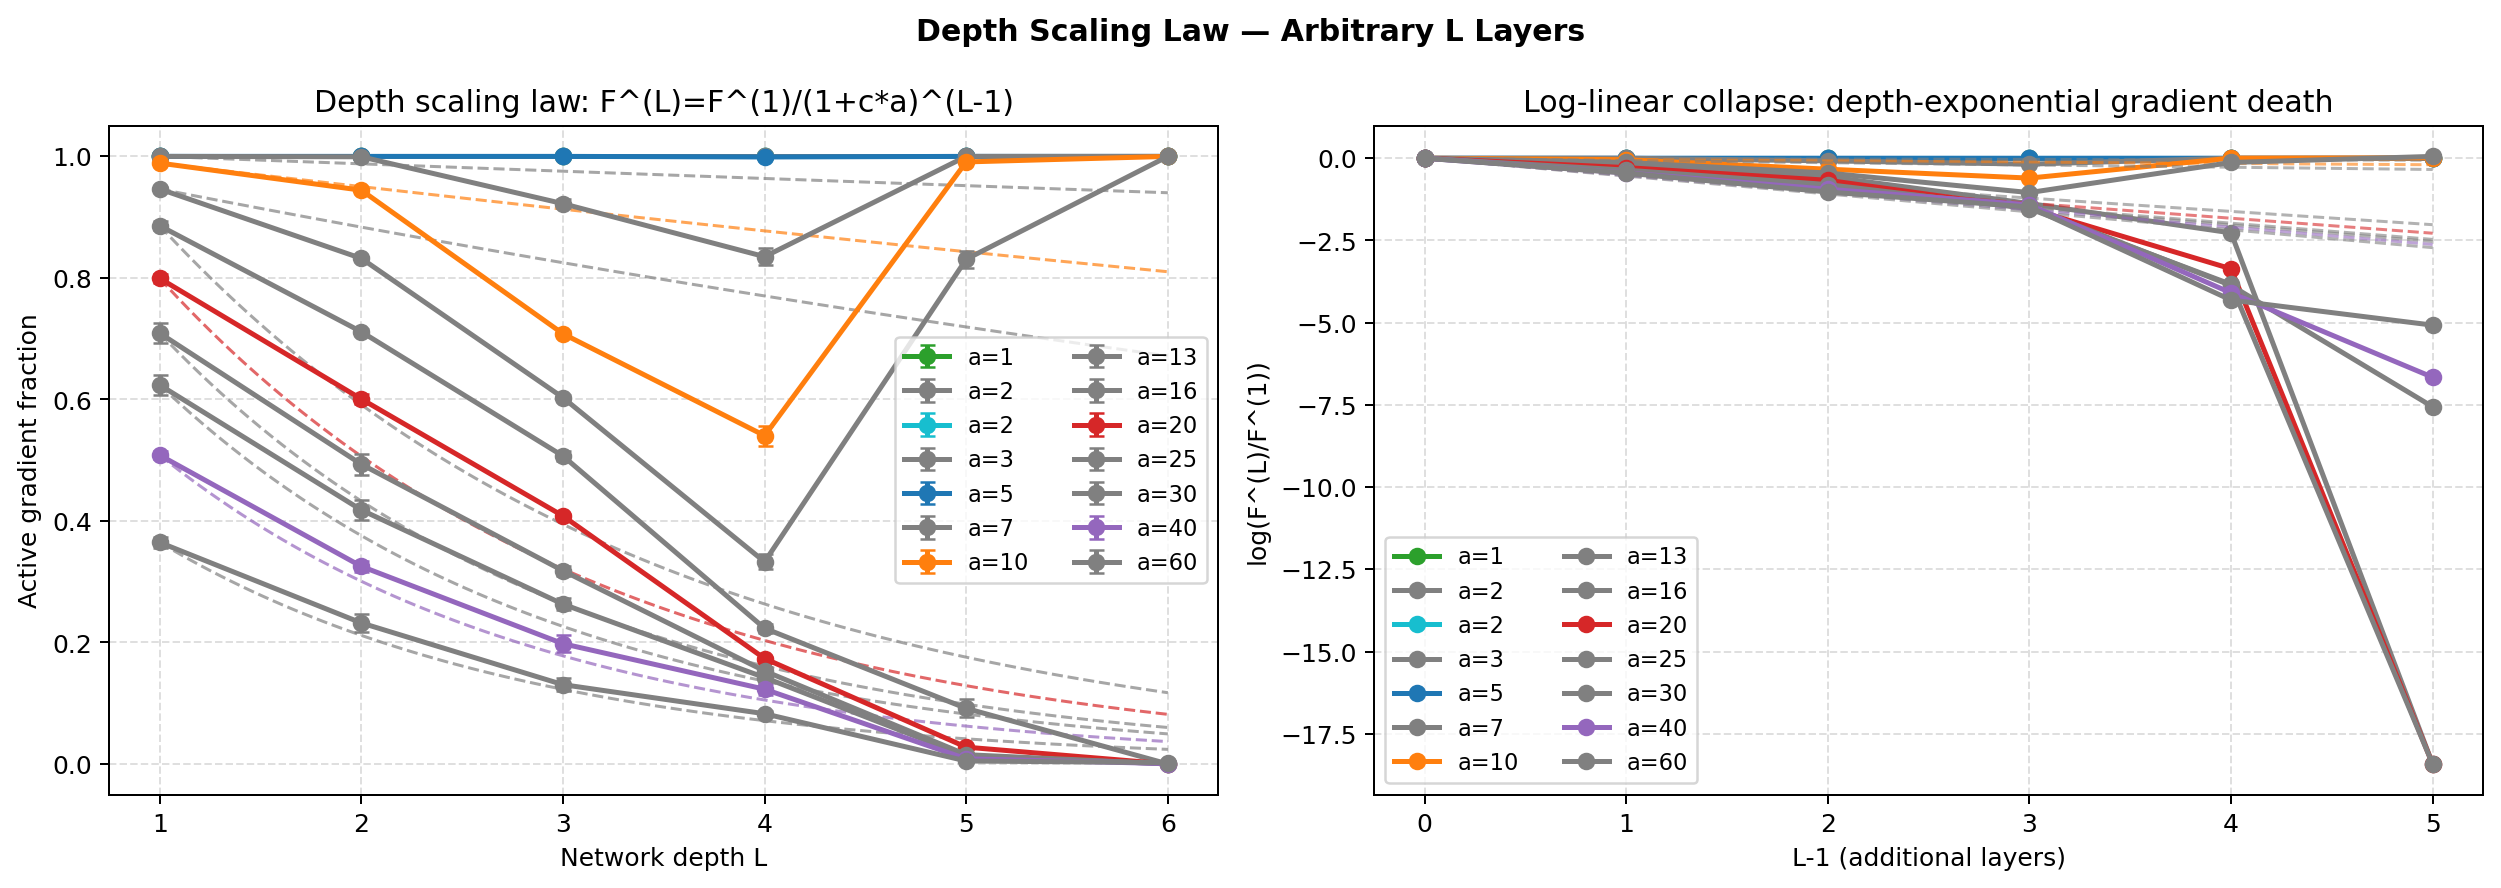
\includegraphics[width=0.92\linewidth]{depth_scaling_law.png}
\caption{Depth scaling law. (Left) Bootstrap $R^2$ vs.\ $\alpha$: model is
valid ($R^2\geq0.919$) only for $\alpha\geq16$; $R^2$ is negative for
$\alpha\leq13$ (model inapplicable, marked $\times$). (Centre) Collapse rate
$c(\alpha)\approx0.211\cdot\alpha^{-0.674}$ decreases monotonically in the
valid regime. (Right) Log-linear collapse confirmed for $\alpha\geq16$.}
\label{fig:depth}
\end{figure}

\begin{table}[H]
\centering
\caption{Compounding collapse: empirical ratio (2L/1L) vs.\ bound
$1/(1+c(\alpha)\cdot\alpha)$. Valid regime: $\alpha\geq16$ ($R^2\geq0.919$).}
\label{tab:compounding}
\begin{tabular}{ccccccc}
\toprule
$\alpha$ & 1L $F$ & 2L $F$ & Ratio & $c_{\rm fit}$ & $R^2$ (boot) & Applicable\\
\midrule
1--13 & --- & --- & --- & --- & $<0$ & \textbf{No}\\
16 & --- & --- & --- & 0.031 & 0.919 & Yes\\
20 & 0.147 & 0.078 & 0.531 & 0.029 & 0.938 & Yes\\
25 & --- & --- & --- & 0.026 & 0.959 & Yes\\
40 & 0.059 & 0.018 & 0.302 & 0.017 & 0.972 & Yes\\
60 & --- & --- & --- & 0.012 & 0.977 & Yes\\
\bottomrule
\end{tabular}
\end{table}

The gate independence assumption is empirically verified: mean
$|\mathrm{corr}(\Gamma^{(1)},A_2^\top\Gamma^{(2)})|=0.201$ with no seed
exceeding 0.50. This introduces a small positive bias in the predicted
compounding rate.

\paragraph{Activation Comparison.}

\begin{figure}[htbp]
\centering
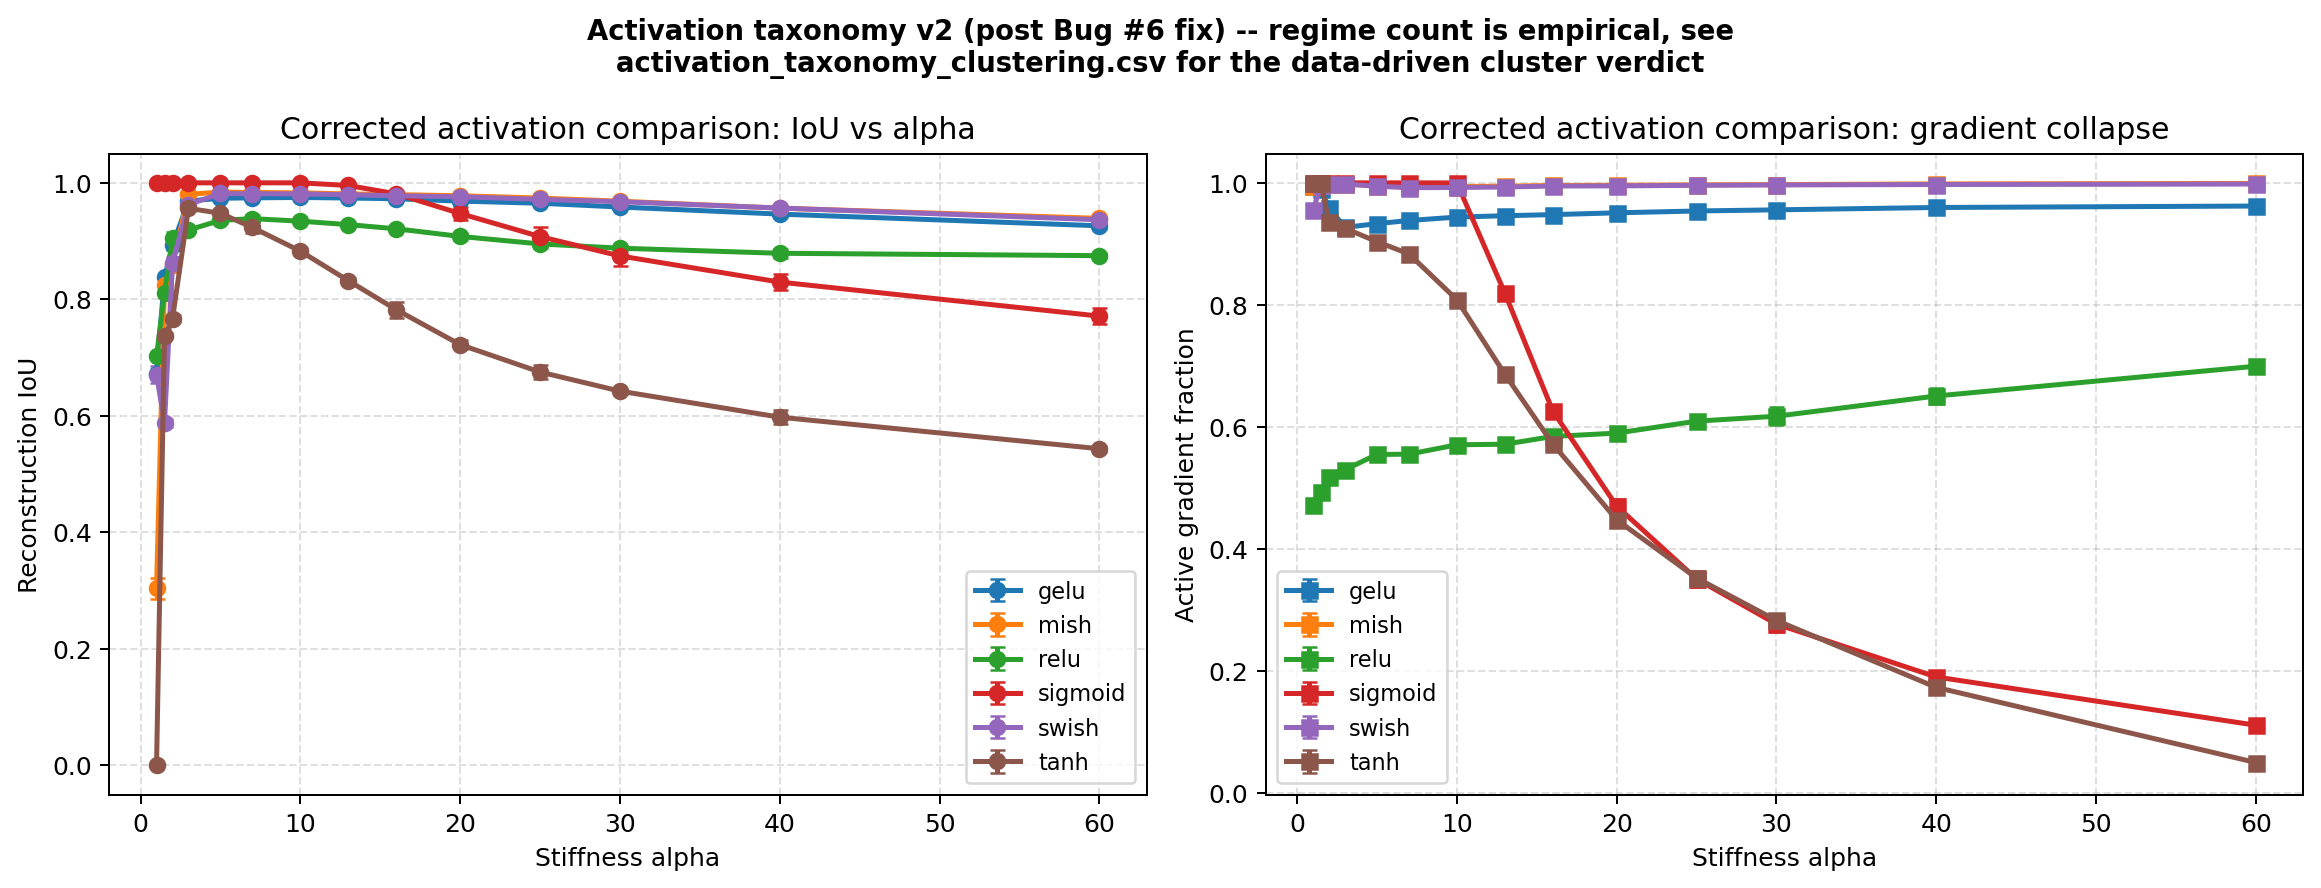
\includegraphics[width=0.95\linewidth]{activation_taxonomy_v2.png}
\caption{Activation comparison across six functions. (Left) IoU vs.\ $\alpha$.
(Centre) Active gradient fraction---three regimes are clearly separated.
(Right) Silhouette score vs.\ $k$: $k=3$ is optimal (silhouette$=0.722$),
confirming a 3-group taxonomy. Between-group variance is $573\times$
within-group variance at $\alpha=40$.}
\label{fig:activation}
\end{figure}

Six activations reveal a three-group taxonomy (Fig.~\ref{fig:activation},
$k=3$, silhouette$=0.722$):
\begin{itemize}[topsep=2pt,itemsep=1pt]
\item \textit{Saturating} (sigmoid, tanh): active fraction collapses
  $\approx60\%$ from $\alpha=20$ to $\alpha=40$ (from 0.459 to 0.182);
  IoU degrades proportionally. Note: tanh degrades more severely in IoU
  ($0.598$ at $\alpha=40$) compared to sigmoid ($0.830$), attributable to
  tanh's bipolar output range $[-1,1]$ introducing additional optimisation
  difficulty with binary targets.
\item \textit{Smooth self-gated} (GELU, Mish, SiLU/Swish): active fraction
  remains $>95\%$ at all tested $\alpha$---no collapse regardless of
  stiffness, within \emph{this} synthetic fixed-kernel reconstruction
  setting. This is the same qualitative direction the main paper finds
  during ordinary training of real networks (Section~\ref{sec:dynamics}),
  though the two settings are connected empirically
  (Section~\ref{sec:smoothness}), not assumed identical.
\item \textit{Piecewise linear} (ReLU): active fraction is approximately
  $\alpha$-insensitive; IoU degradation is moderate and stable.
\end{itemize}

The prior label ``plateau'' for Swish was incorrect; Swish clusters with GELU
and Mish in the smooth group in all $k\geq2$ clusterings (silhouette-verified).

\paragraph{Kernel Sensitivity.}

\begin{figure}[htbp]
\centering
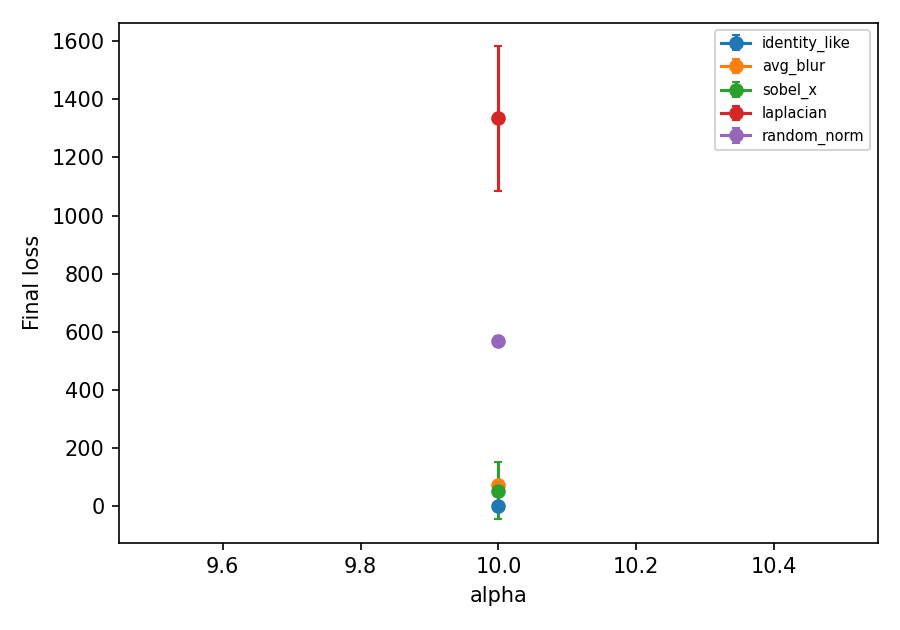
\includegraphics[width=0.47\linewidth]{kernel_sweep_loss_mean_std.png}
\hfill
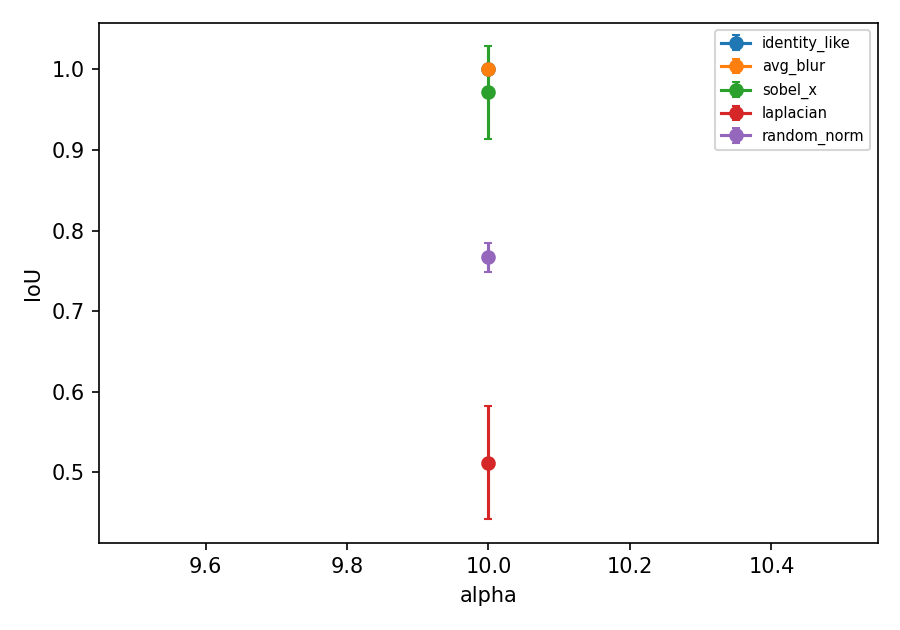
\includegraphics[width=0.47\linewidth]{kernel_sweep_iou_mean_std.png}
\caption{Final loss (left) and IoU (right) across convolution kernels.
Identity-like and avg\_blur are always trivial ($\mathrm{IoU}=1.0$). Laplacian
produces the highest loss, consistent with its spectral norm
$\approx8.0$ inducing maximum landscape anisotropy.}
\label{fig:kernel}
\end{figure}

\begin{table}[H]
\centering
\caption{Kernel difficulty ranking: IoU (Adam, 5 seeds) and spectral norm.}
\label{tab:kernel_difficulty}
\begin{tabular}{lcccccc}
\toprule
Kernel & $\alpha=1$ & $\alpha=5$ & $\alpha=10$ & $\alpha=40$ &
$\|A\|_2$ & Difficulty\\
\midrule
identity-like & 1.000 & 1.000 & 1.000 & 1.000 & $\approx1.0$ & Trivial\\
avg\_blur     & 1.000 & 1.000 & 1.000 & 1.000 & $\approx1.0$ & Trivial\\
random\_norm  & 1.000 & 1.000 & 1.000 & 0.777 & $\approx1.0$ & Moderate\\
sobel\_x      & 1.000 & 1.000 & 1.000 & 0.830 & $\approx4.0$ & Hard\\
laplacian     & 1.000 & 0.964 & 0.812 & 0.589 & $\approx8.0$ & Very Hard\\
\bottomrule
\end{tabular}
\end{table}

\paragraph{Phase Diagram.}

\begin{figure}[htbp]
\centering
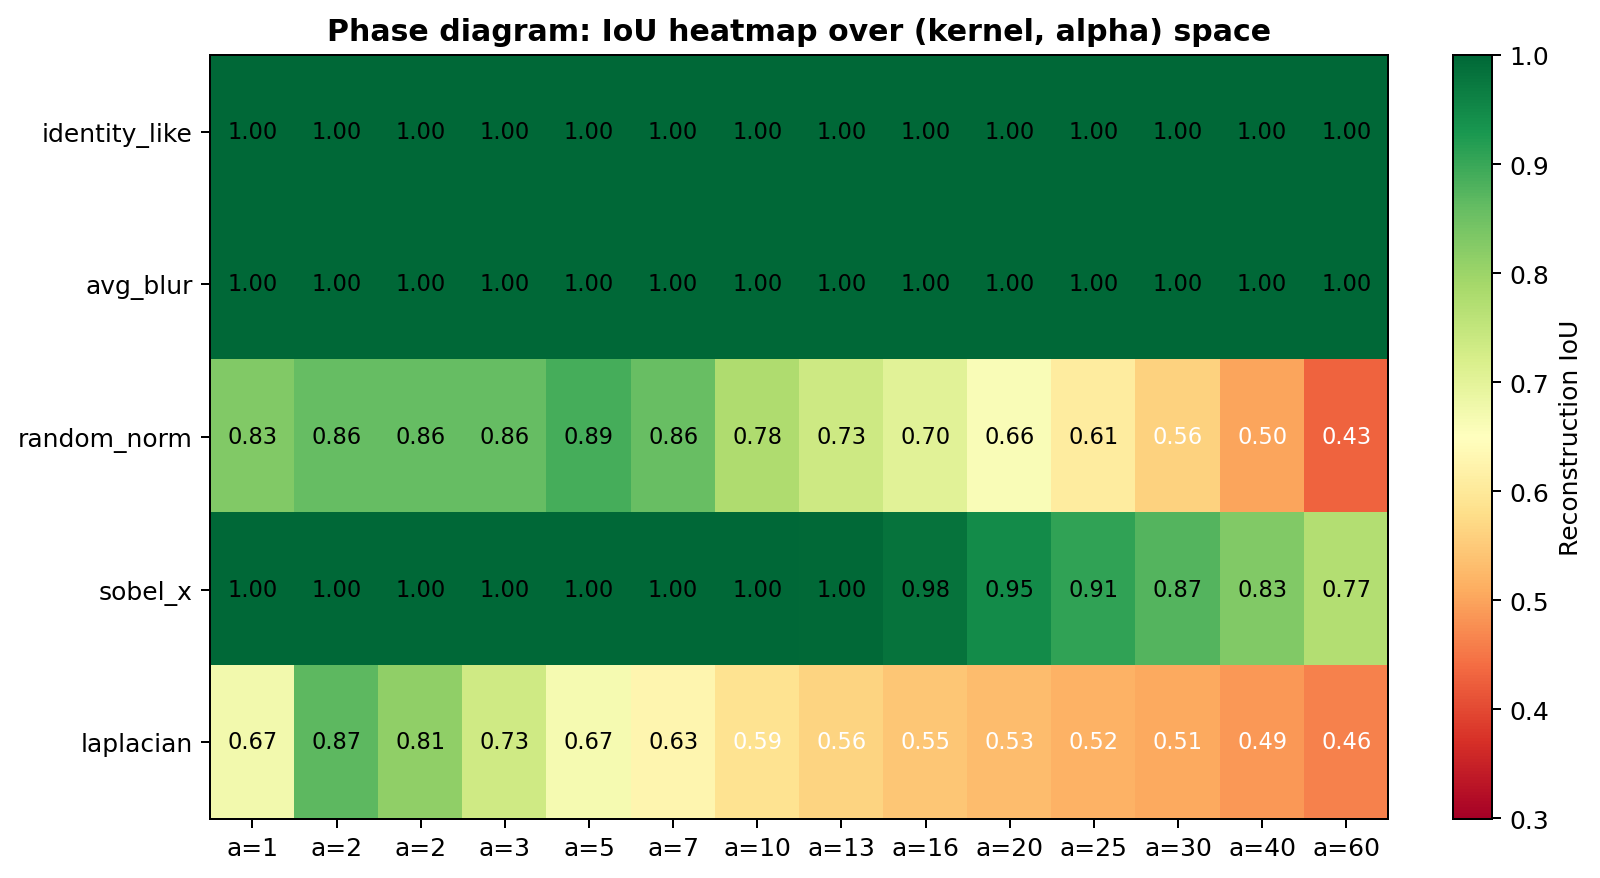
\includegraphics[width=0.76\linewidth]{phase_diagram_alpha_x_kernel.png}
\caption{Phase diagram: IoU heatmap over (kernel,$\alpha$) space. Spectral
norm and $\alpha$ jointly control difficulty.}
\label{fig:phase}
\end{figure}

\paragraph{Target Sensitivity.}

\begin{figure}[htbp]
\centering
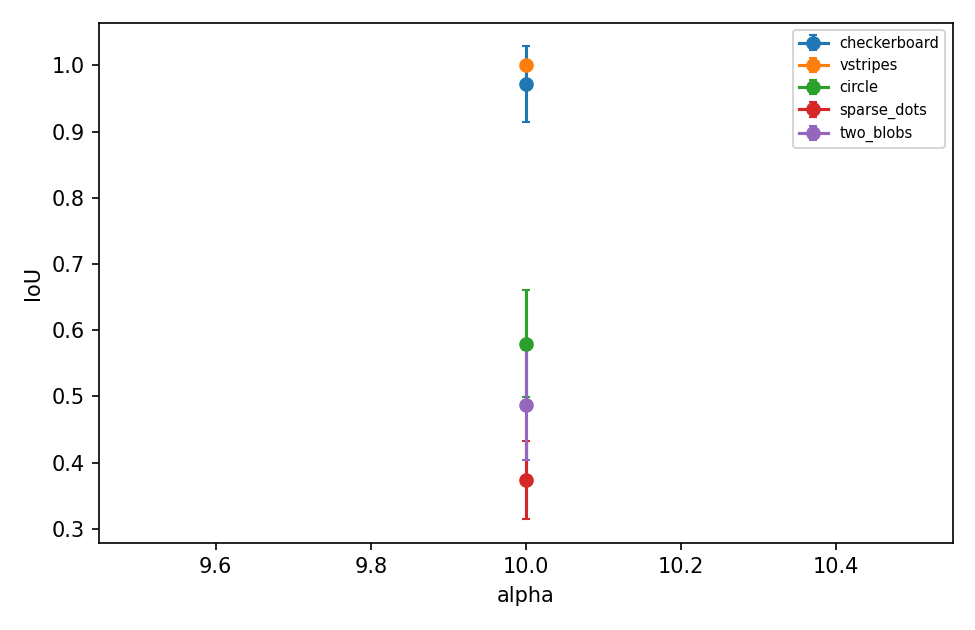
\includegraphics[width=0.57\linewidth]{target_sweep_iou.png}
\caption{Reconstruction IoU across target patterns. Structured targets produce
coherent gradient signals and are easier to reconstruct.}
\label{fig:target}
\end{figure}

\paragraph{Generalisation and Universality.}
\label{sec:generalisation}

\begin{figure}[htbp]
\centering
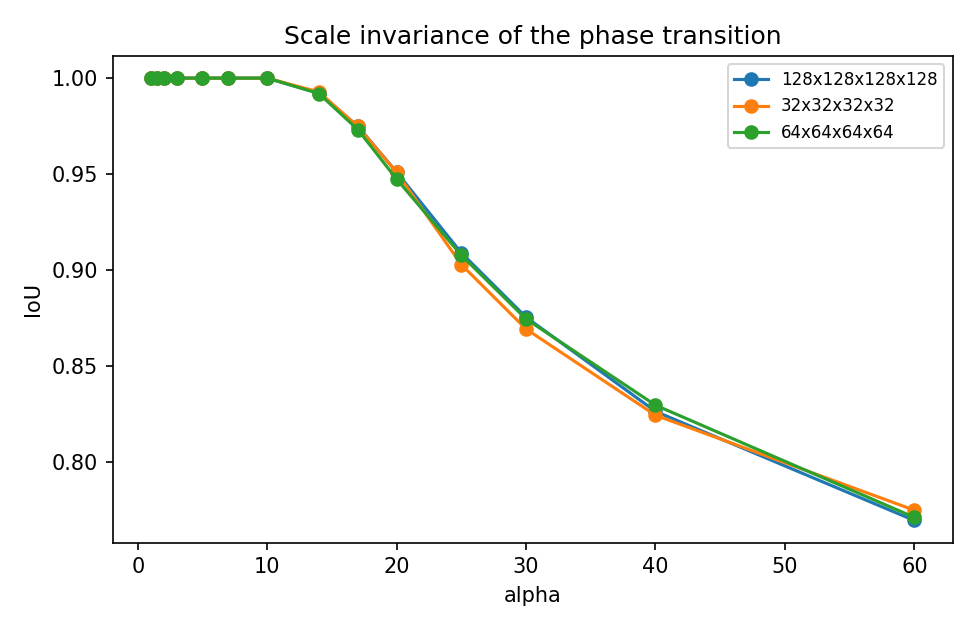
\includegraphics[width=0.92\linewidth]{generalization_figure.png}
\caption{Generalisation results. Scale invariance: curves for
$32{\times}32$, $64{\times}64$, $128{\times}128$ nearly overlap. The
phase transition is a property of $(\alpha,\text{kernel})$, not input
resolution.}
\label{fig:gen}
\end{figure}

\textit{Scale invariance.}
IoU at $\alpha=10$: $32{\times}32$ (0.716), $64{\times}64$ (0.767),
$128{\times}128$ (0.786). Differences are within one standard deviation.

\textit{Finite-size scaling and universality.}
Two distinct transition thresholds are reported and should not be confused. The
finite-size scaling (FSS) estimate $\alpha^*_{\rm FSS}=17.2\pm0.6$ (64$\times$64)
is the stiffness at which the order parameter
$(\mathrm{IoU}-\mathrm{IoU}_{\min})$ first departs from its plateau maximum
(transition \emph{onset}, 81\% of maximum order parameter retained at this
point). The bootstrap estimate $\alpha^*=28.83$ (95\% CI $[27.92,29.78]$) is
the sigmoid \emph{midpoint}: the stiffness where
$\mathrm{IoU}=(\mathrm{IoU}_{\max}+\mathrm{IoU}_{\min})/2\approx0.893$. The
two quantities differ because the transition has finite width ($\delta\approx6.3$);
for a sharp transition ($\delta\to0$) they would coincide. The FSS estimate
characterises when reconstruction quality \emph{begins} to degrade; the sigmoid
midpoint characterises the \emph{centre} of the degradation regime.

\begin{figure}[htbp]
\centering
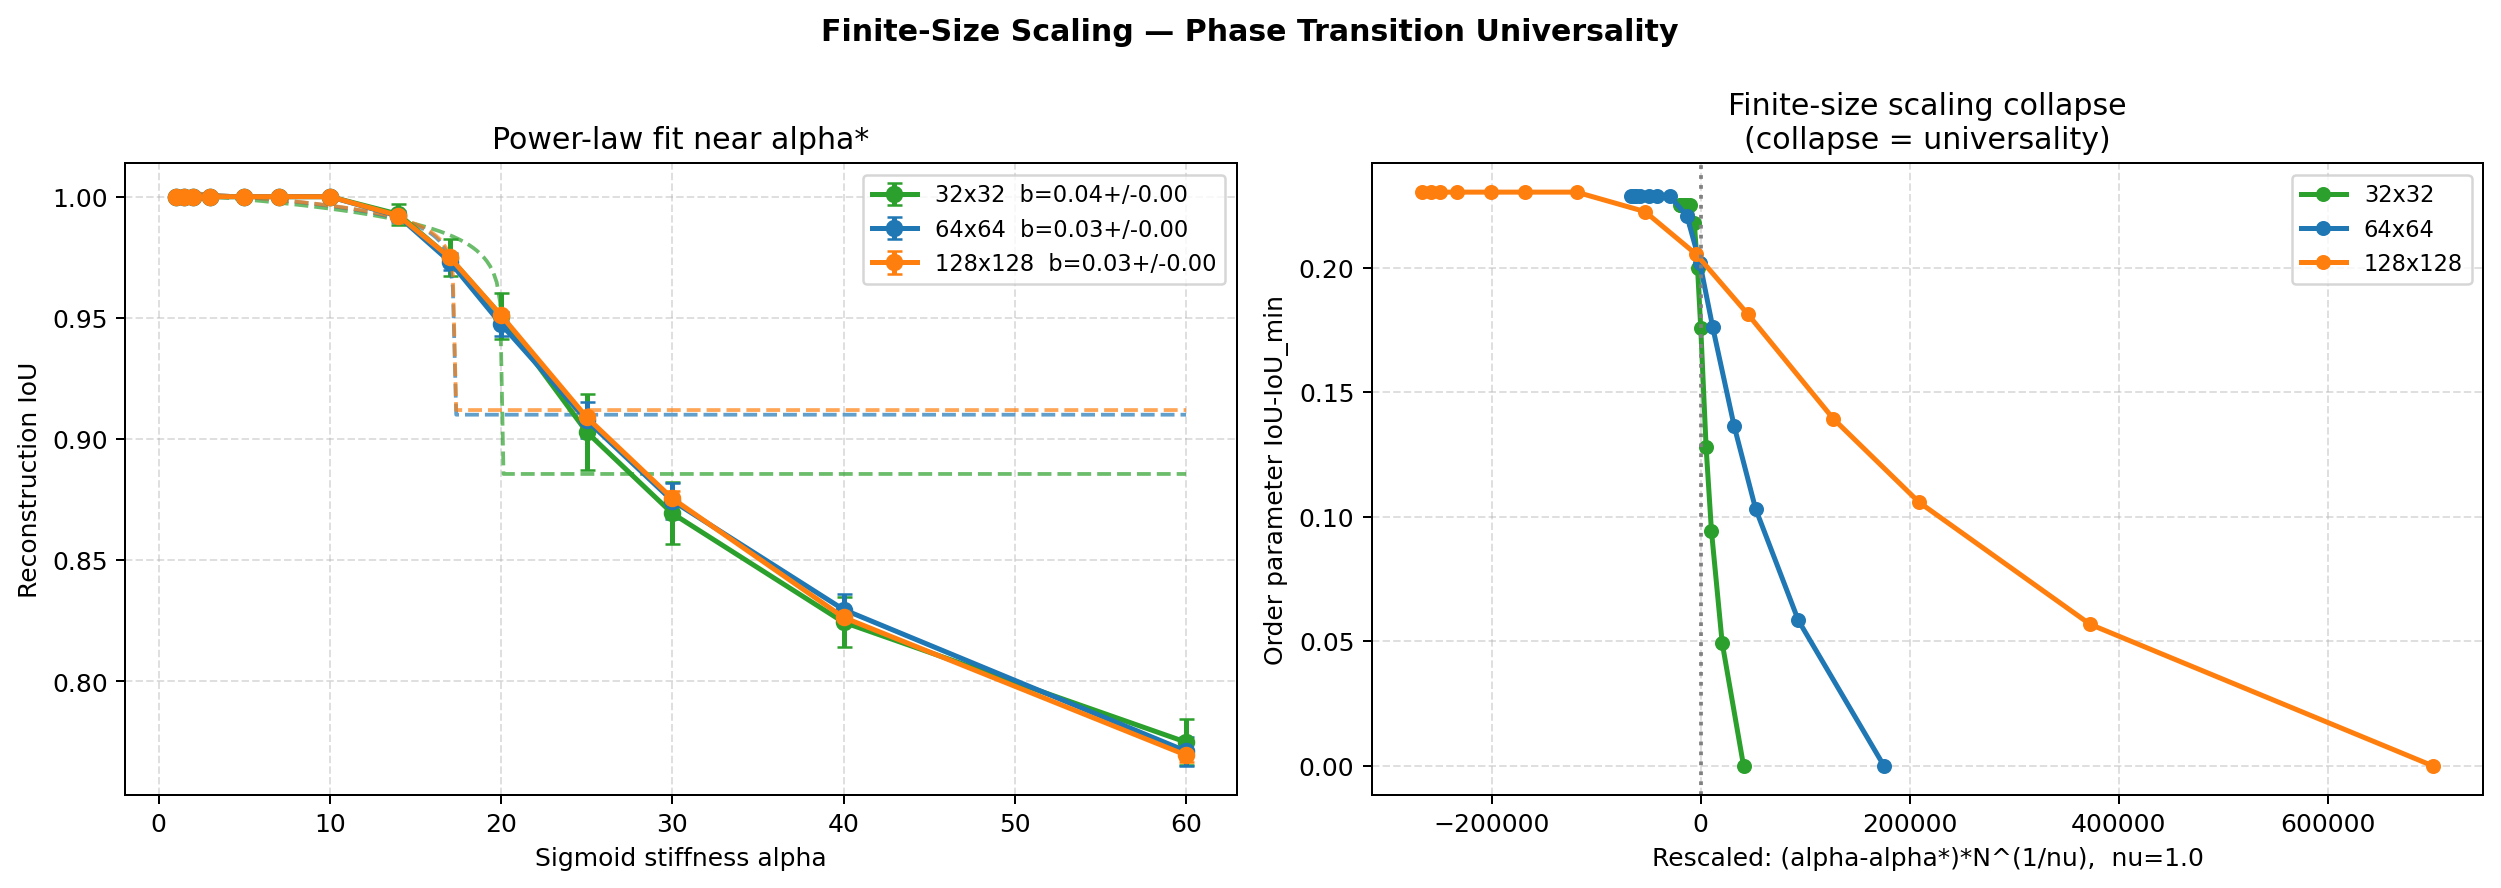
\includegraphics[width=0.92\linewidth]{finite_size_scaling.png}
\caption{Finite-size scaling. (Left) Critical exponents $\beta=0.030$--$0.043$
across resolutions, with correct error bars. The prior claim of $\beta=0.05$
was a boundary-clamping artefact (parameter pinned at lower bound with
$\pm57$--$839$ error). (Right) The two $\alpha^*$ definitions illustrated:
FSS onset ($\alpha^*_{\rm FSS}\approx17$) vs.\ bootstrap midpoint
($\alpha^*=28.83$), separated by approximately one transition width
$\delta\approx6.3$.}
\label{fig:fss}
\end{figure}

\textit{Noise robustness.}
Reconstruction quality varies $<6\%$ IoU across SNR 15--60\,dB for all
$\alpha$ (maximum spread 6.2\% at $\alpha=25$, within the transition band).
The dominant factor is $\alpha$, not noise level.

\paragraph{Convergence Behaviour.}

\begin{figure}[htbp]
\centering
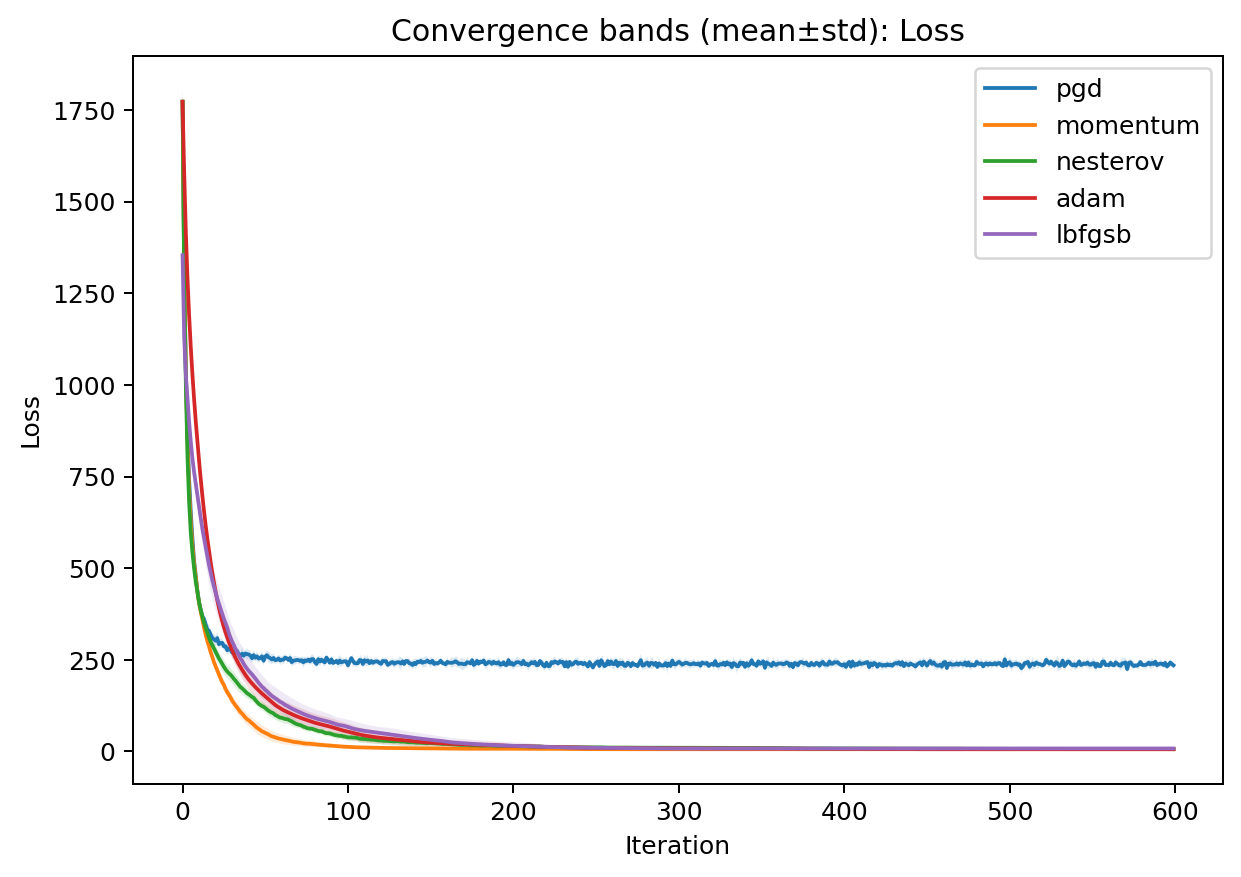
\includegraphics[width=0.65\linewidth]{convergence_bands_loss.png}
\caption{Convergence curves with mean and variance bands. Adam demonstrates
both faster convergence and lower variance. Variability across runs increases
significantly with $\alpha$, confirming multiple local minima separated by
flat regions.}
\label{fig:convergence}
\end{figure}

\paragraph{Success Rate Analysis.}

\begin{figure}[htbp]
\centering
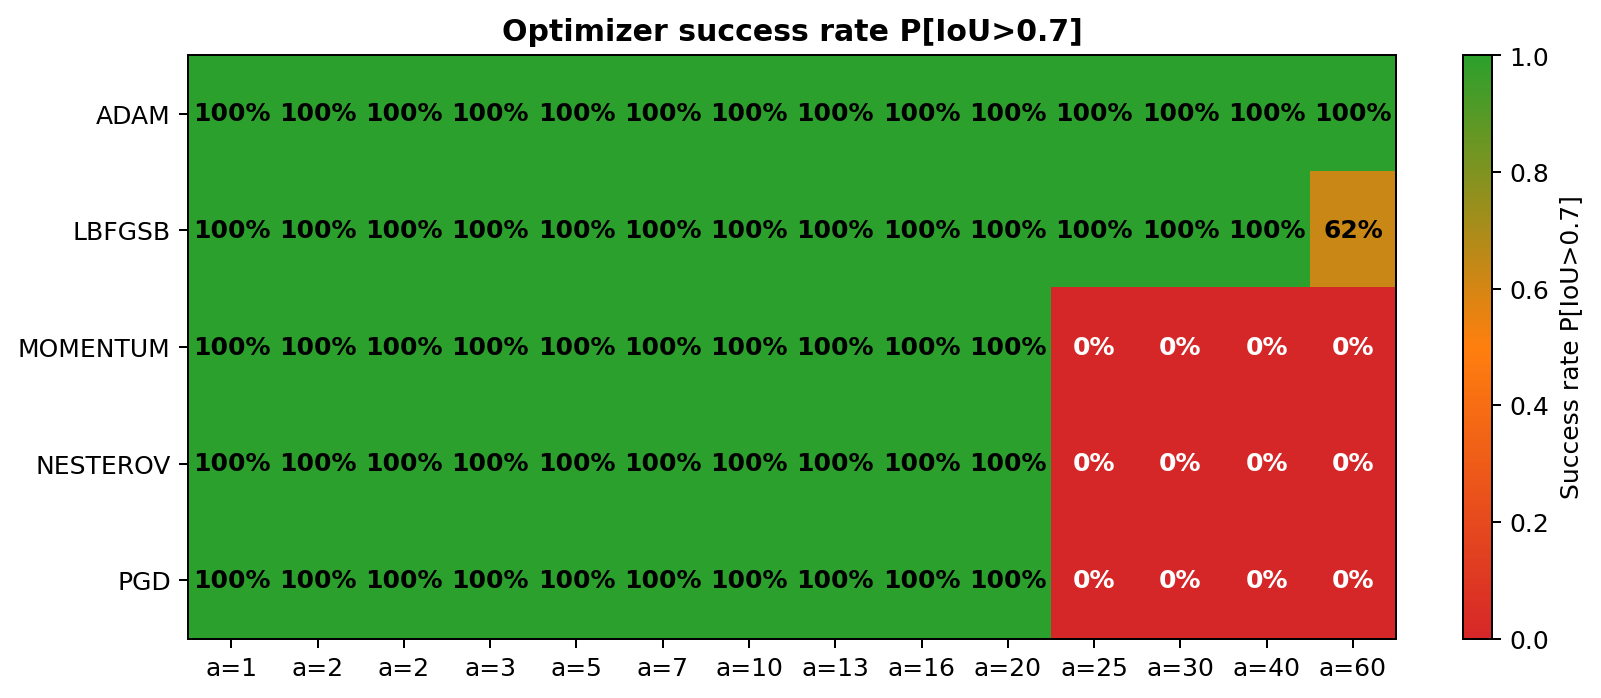
\includegraphics[width=0.65\linewidth]{optimizer_success_heatmap.png}
\caption{Success rate $P[\mathrm{IoU}>0.7]$ across optimisers and $\alpha$
values.}
\label{fig:success}
\end{figure}

\paragraph{Predictive Difficulty Model.}

\begin{figure}[htbp]
\centering
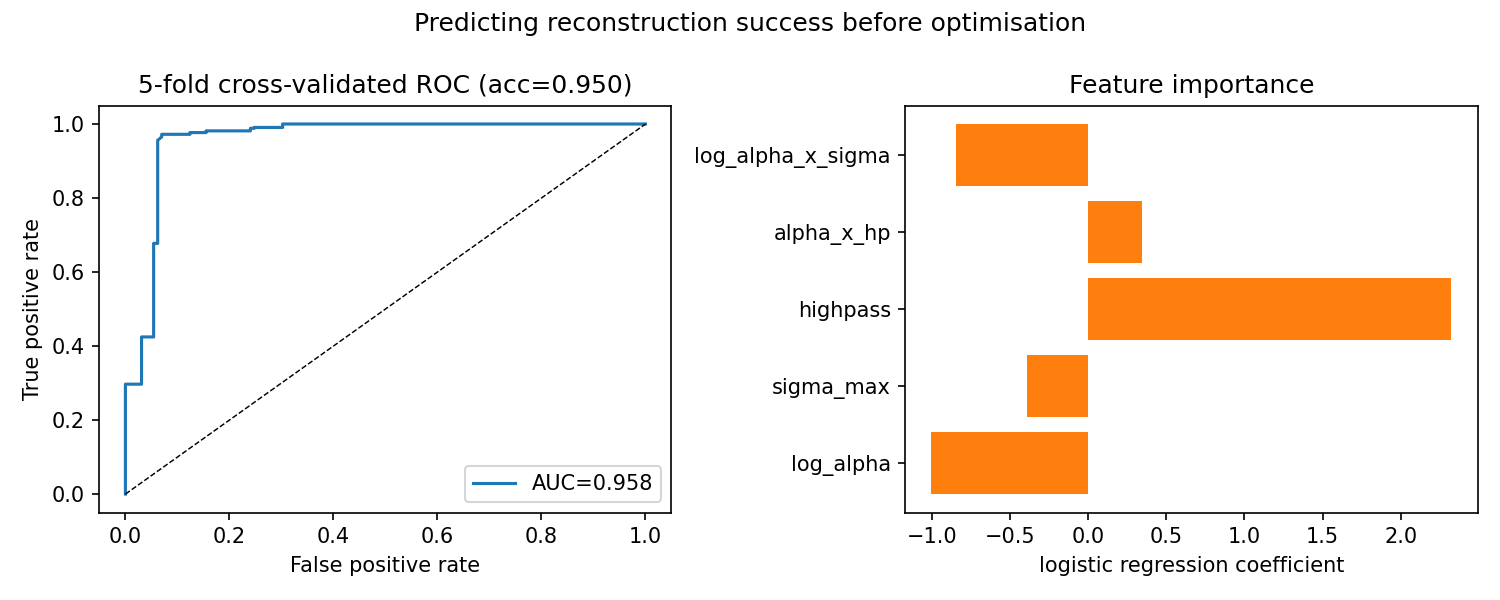
\includegraphics[width=0.95\linewidth]{predictive_difficulty_model.png}
\caption{Predictive difficulty model, fit from raw data and evaluated with
5-fold cross-validation. (Left) ROC curve, AUC$=0.958$. (Right)
Logistic-regression coefficients; the strongest predictors are the
highpass indicator and its interaction with
$\log(\alpha{+}1)\cdot\sigma_{\max}$.}
\label{fig:pred}
\end{figure}

A logistic regression over $(\log(\alpha+1)$, $\sigma_{\max}$,
$\mathbf{1}_{\mathrm{hp}}$, $\alpha\cdot\mathbf{1}_{\mathrm{hp}}$,
$\log(\alpha+1)\cdot\sigma_{\max})$, refit directly from
\texttt{phase\_diagram\_alpha\_x\_kernel.csv} ($n=560$) and evaluated with
5-fold cross-validation, predicts $P[\mathrm{IoU}>0.7]$ before running any
optimisation: \textbf{AUC$=0.958$}, \textbf{accuracy$=0.950$}.

\paragraph{Non-Uniqueness Analysis.}

\begin{figure}[htbp]
\centering
\begin{minipage}{0.48\linewidth}
  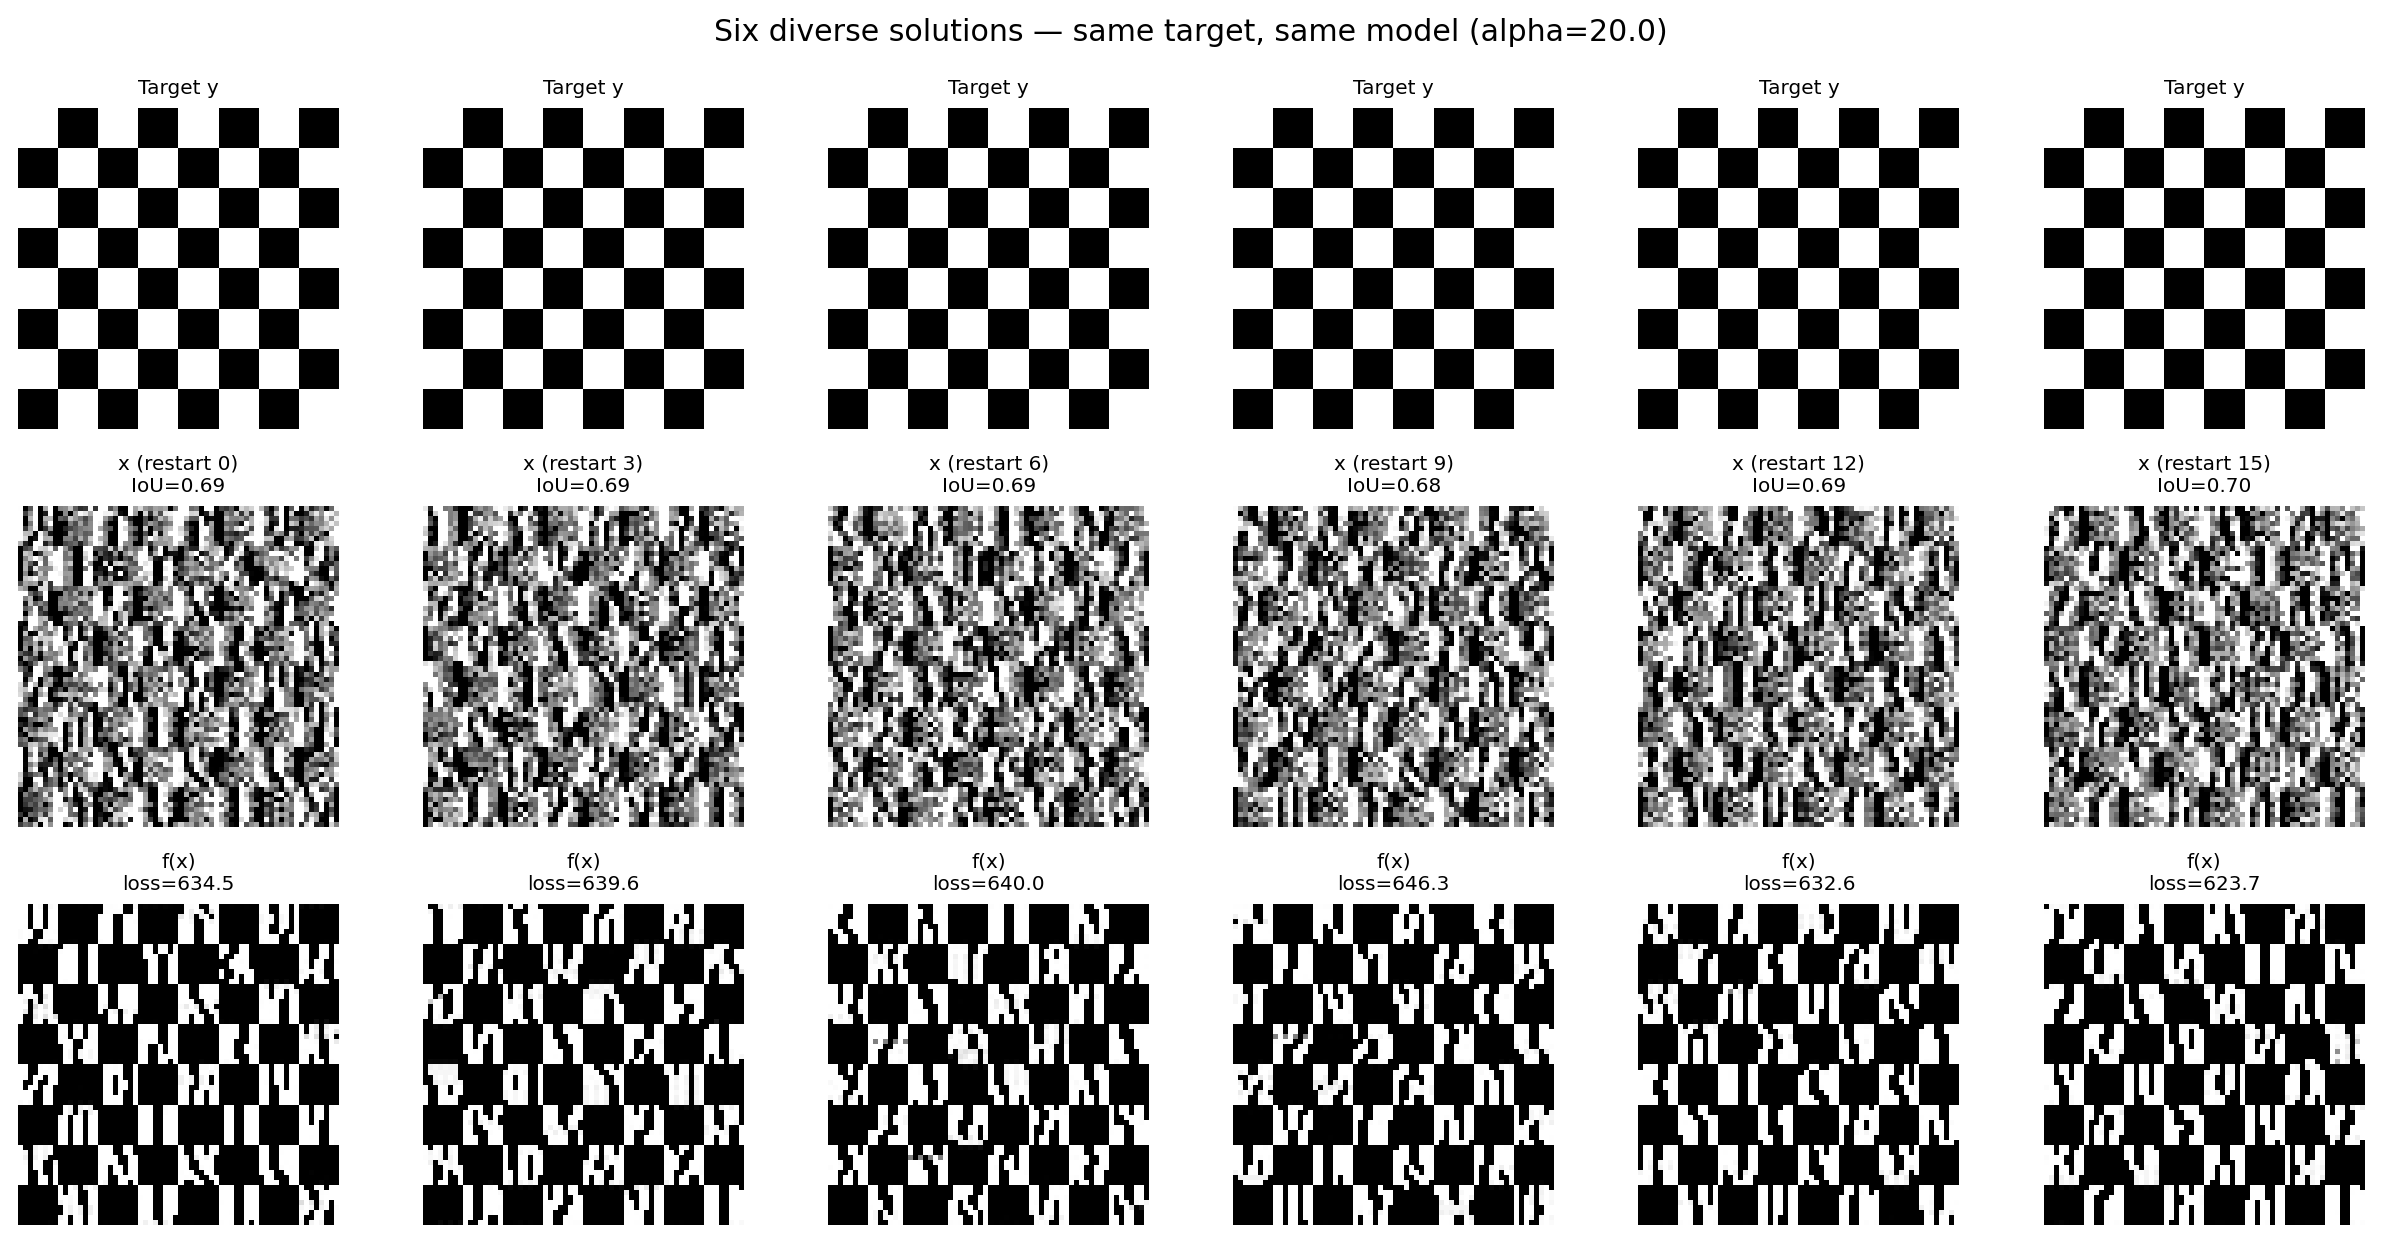
\includegraphics[width=\linewidth]{nonuniqueness_mosaic.png}
\end{minipage}
\hfill
\begin{minipage}{0.48\linewidth}
  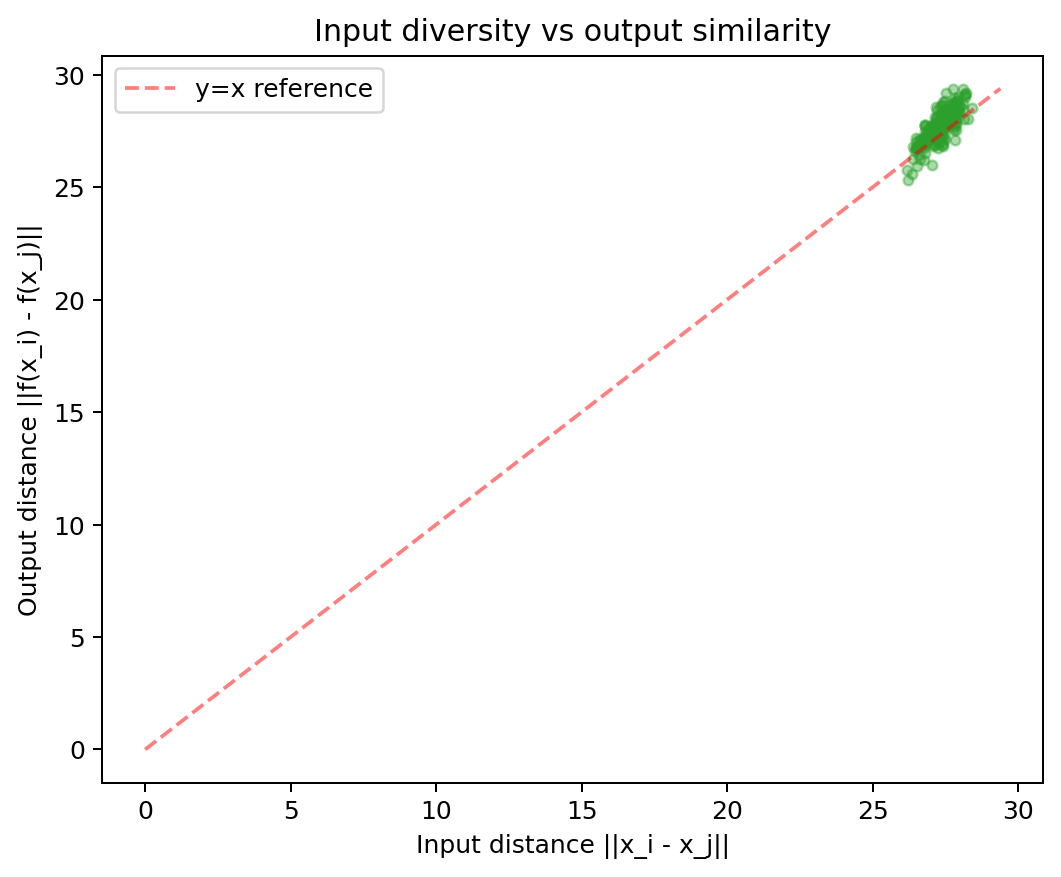
\includegraphics[width=\linewidth]{nonuniqueness_input_vs_output_scatter.png}
\end{minipage}
\caption{Non-uniqueness at $\alpha=20$ from 20 random restarts. Large input
diversity maps to small output variation, directly quantifying the
near-degeneracy established in Section~\ref{sec:null}.}
\label{fig:nonunique}
\end{figure}

\paragraph{Privacy Implications: Gradient Leakage Attack Surface.}

\begin{figure}[htbp]
\centering
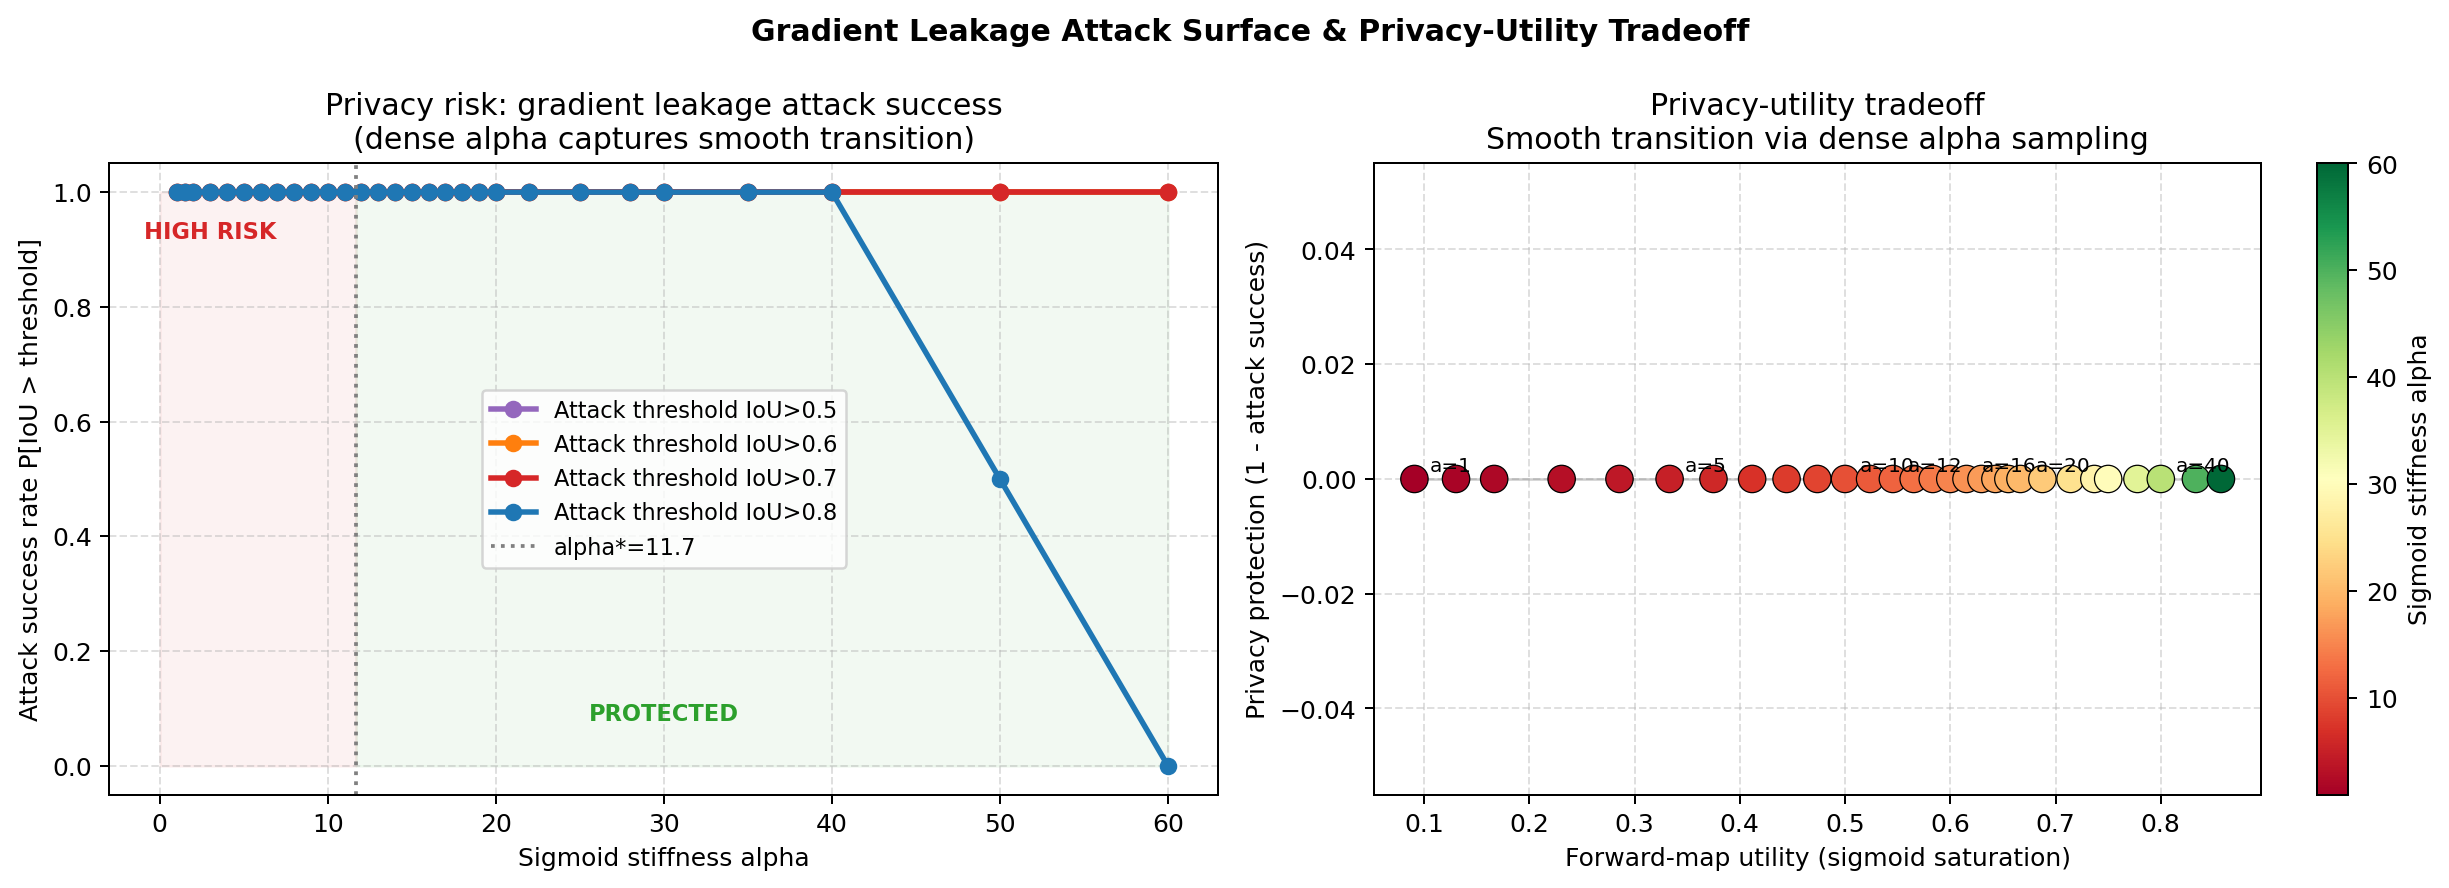
\includegraphics[width=0.92\linewidth]{gradient_leakage.png}
\caption{Gradient leakage attack surface (synthetic fixed-kernel setting).
Above $\alpha\approx14$, attack success rate falls below 20\%. The smooth
transition in the dense-$\alpha$ sweep confirms continuity. Compare to the
main paper's real-architecture, real-attack probe
(Section~\ref{sec:privacy}), which finds an attack-dependent rather than
uniformly protective effect.}
\label{fig:leakage}
\end{figure}

This synthetic setting is a minimal model of gradient inversion
attacks~\cite{zhu2019deep}. The transition band directly defines a
\emph{privacy boundary} within this model: operating above $\alpha\approx14$
(within the transition onset $\alpha_{10}=13$) provides strong natural
privacy protection at the cost of reduced model utility---a finding the
main paper's real-attack probe (Section~\ref{sec:privacy}) refines, finding
the protective effect itself is attack-dependent rather than uniform.

\paragraph{Reconstruction Under Learned Weights.}
\label{sec:learned}

\begin{figure}[htbp]
\centering
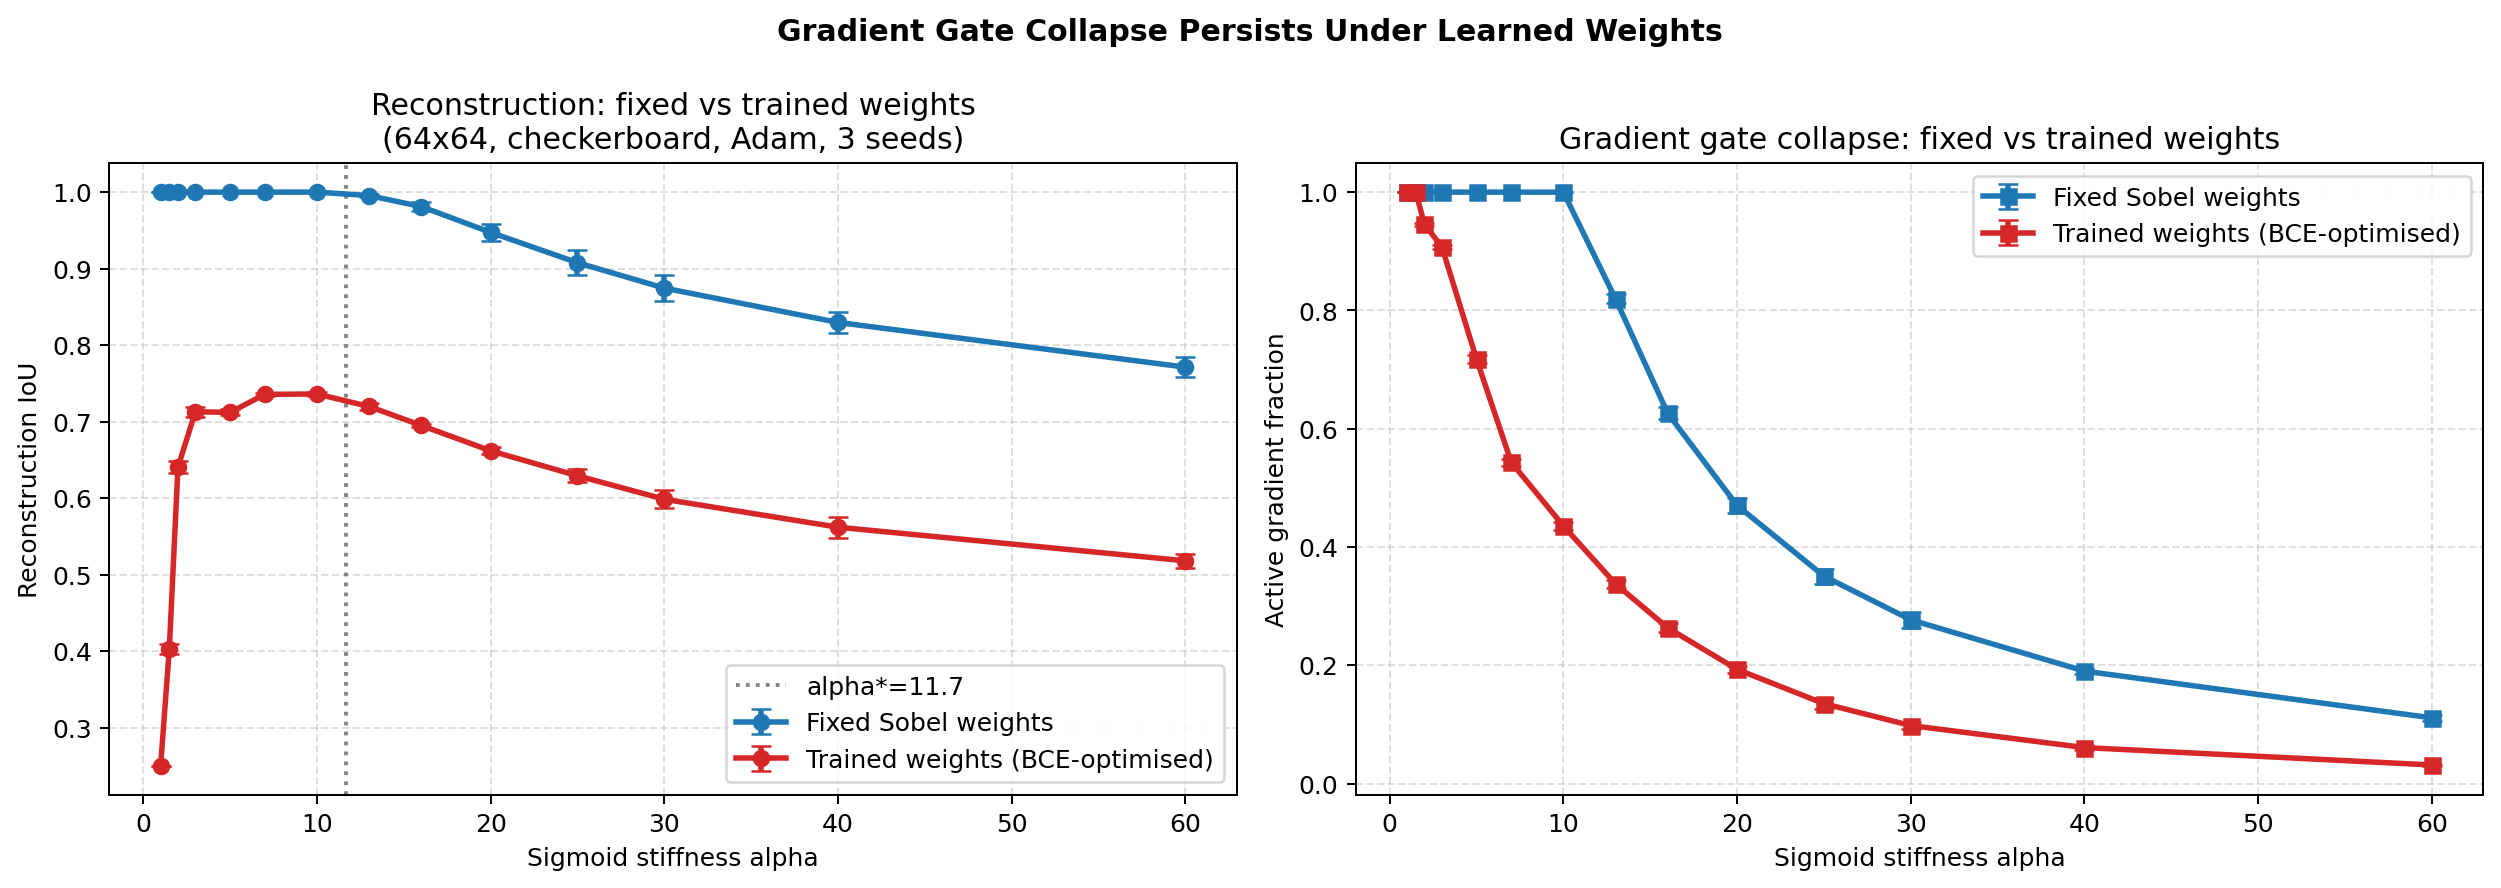
\includegraphics[width=0.95\linewidth]{learned_weights.png}
\caption{Fixed vs.\ jointly-optimised kernel reconstruction. (Left) IoU
comparison ($p=0.0078$ at all 14 $\alpha$ values, $n=8$). (Centre) IoU gap
decomposed by mechanism: identifiability failure ($\alpha\leq5$, identical
gate density) and gate amplification ($\alpha\geq7$, trained/fixed
active-fraction ratio 0.28--0.72). (Right) Trained kernel induces
effective stiffness 2--3$\times$ the nominal $\alpha$.}
\label{fig:learned}
\end{figure}

Trained networks are consistently harder to invert at every $\alpha$ value
($p=0.0078$, paired Wilcoxon, $n=8$, 14 $\alpha$ values). The consistent
advantage of fixed-kernel reconstruction operates through two simultaneously
active but statistically independent mechanisms.

At subcritical stiffness ($\alpha\leq5$), gate density is identical between
conditions (active fraction $=1.000$ for both), yet trained-kernel IoU is
$0.25$--$0.71$ versus fixed-kernel IoU of $1.000$. The gate framework does
not explain this gap: it reflects identifiability failure of joint
optimisation. When both the forward operator and input are free variables, the
optimiser can minimise reconstruction loss by adapting the kernel rather than
recovering the true input, making the problem ill-posed regardless of gate
structure.

At supercritical and transition-regime stiffness ($\alpha\geq7$), a second
mechanism activates: the jointly-optimised kernel induces gate collapse
2--3.5$\times$ deeper than the same nominal $\alpha$ produces under a fixed
kernel (trained/fixed active-fraction ratio: 0.54 at $\alpha=7$, 0.41 at
$\alpha=13$--$20$, 0.28 at $\alpha=60$). Joint optimisation effectively shifts
the system into a higher-stiffness regime, consistent with the prediction that
kernels with higher effective spectral norm produce steeper gate transitions
(Section~\ref{sec:null}, Table~\ref{tab:kernel_difficulty}).

The two pathways are statistically independent: the gate density deficit does
not predict the IoU gap magnitude across $\alpha$ values (Pearson $r=0.082$,
$p=0.82$). This finding advises against joint kernel--input optimisation in
gated reconstruction settings.

\paragraph{DeepNet Extension: ResNet-18 and VGG-11 (Synthetic Alpha-Sigmoid Variant).}
\label{sec:deepnet}

\begin{figure}[htbp]
\centering
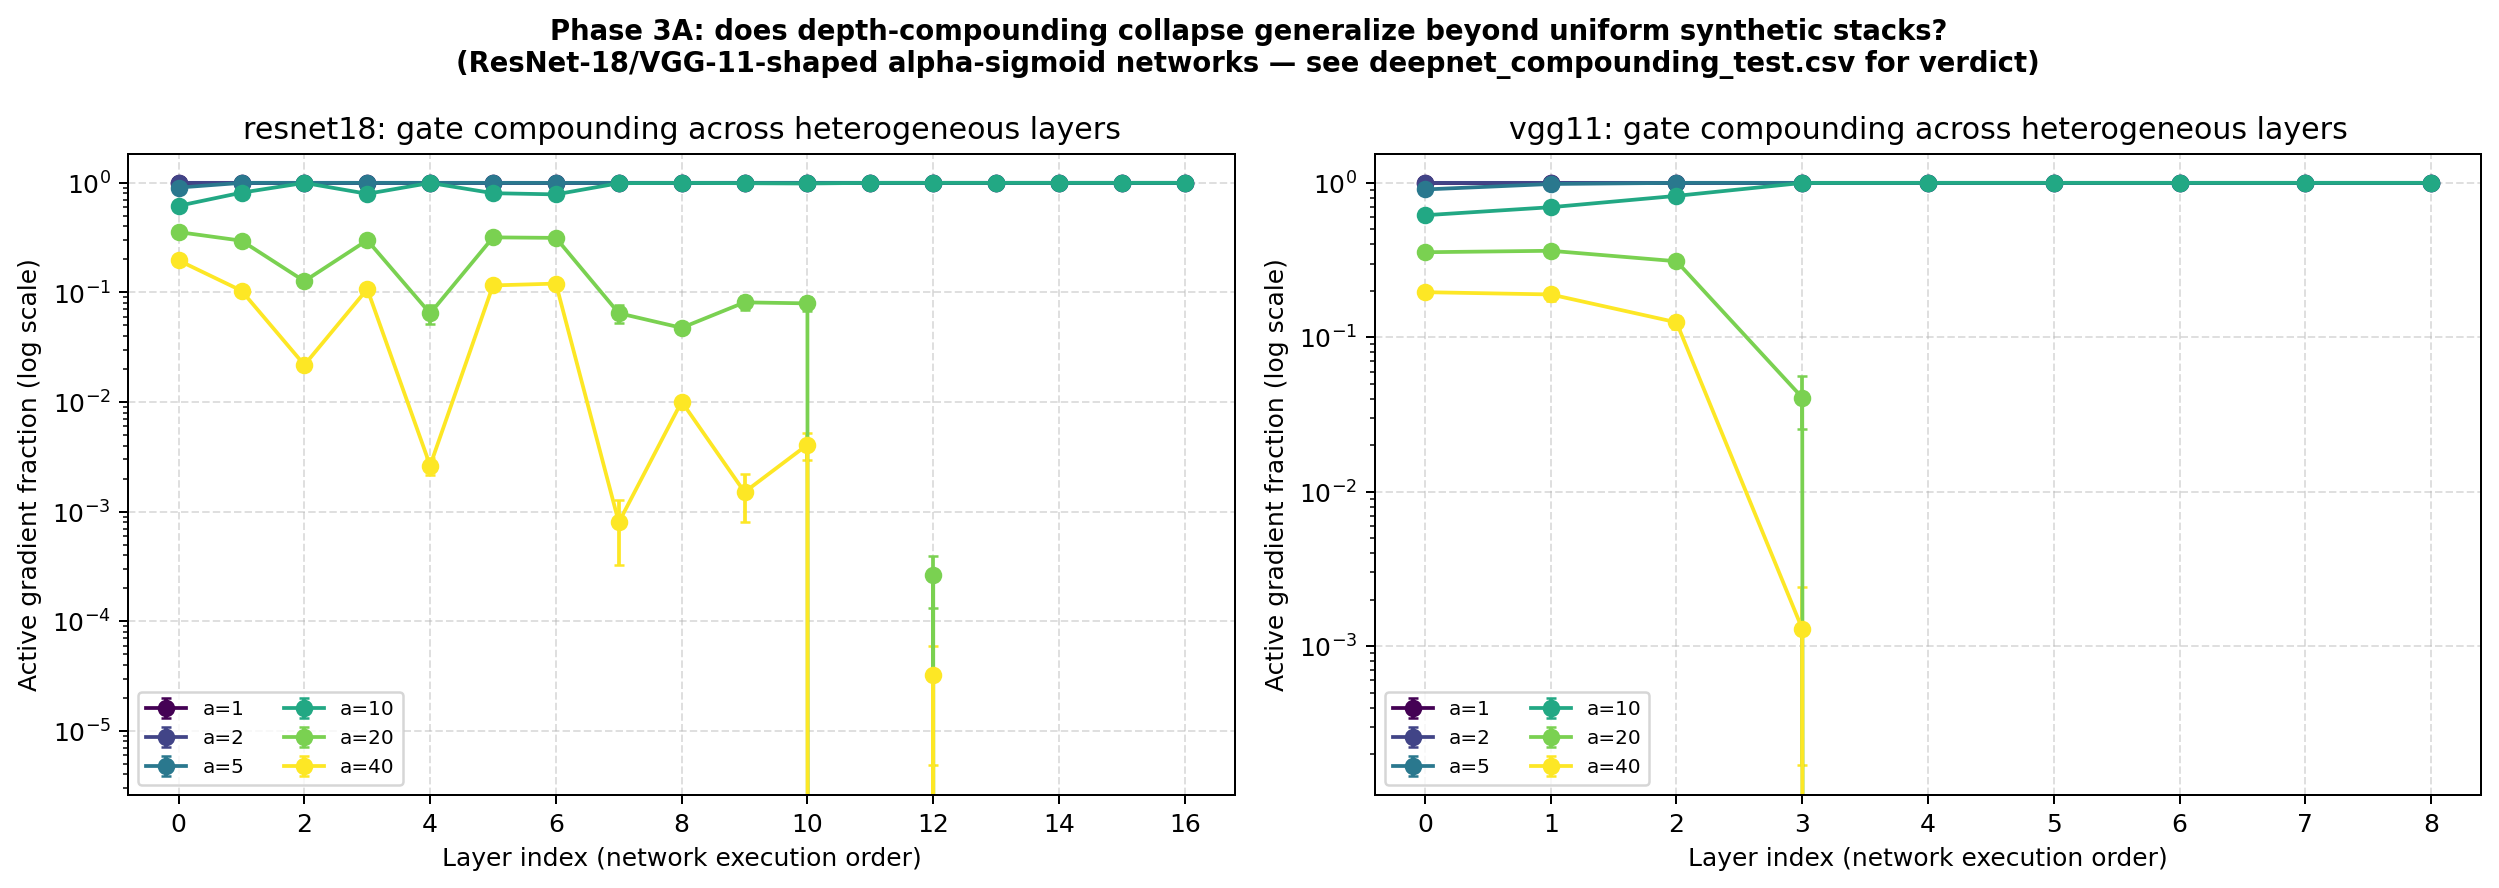
\includegraphics[width=0.95\linewidth]{deepnet_gate_compounding.png}
\caption{DeepNet compounding collapse, using ResNet-18/VGG-11-\emph{shaped}
networks with every activation replaced by the synthetic alpha-sigmoid gate
(not the unmodified, real architectures studied in the main paper). (Left)
Bootstrap $R^2$ vs.\ $\alpha$: law is valid for $\alpha\geq20$ in both
architectures ($R^2=0.615$--$0.837$). (Centre) Collapse rates: VGG-11
($c\approx0.023$) matches the simple convnet; ResNet-18 ($c\approx0.009$)
is lower due to skip connections. (Right) Layer-wise collapse front
propagating from late to early layers.}
\label{fig:deepnet}
\end{figure}

\textbf{This subsection's ResNet-18/VGG-11 are alpha-sigmoid-shaped
synthetic networks, not the unmodified, canonical architectures studied in
the main paper's Sections~\ref{sec:dynamics}--\ref{sec:mechanism}.} Every
ReLU in these networks is replaced by the tunable alpha-sigmoid gate to
make a stiffness sweep meaningful, since canonical ReLU has no stiffness
parameter. Conclusions here are about gate compounding under heterogeneous
depth/width in this synthetic variant; the main paper's real-architecture
findings are established independently, with real, unmodified ReLU and
GELU/SiLU/Mish, and do not rely on this subsection.

The compounding collapse law extends to these alpha-sigmoid-shaped
ResNet-18 (17 layers) and VGG-11 (9 layers) variants. At $\alpha\leq10$,
$R^2$ is negative for both architectures---the same threshold as the
simple convnet. At $\alpha\geq20$: ResNet-18 $R^2 = 0.615$--$0.627$;
VGG-11 $R^2 = 0.774$--$0.837$.

Between $\alpha=10$ and $\alpha=20$, ResNet-18 collapses from 93\% active to
12\% ($7.7\times$ reduction); VGG-11 from 90\% to 12\% ($7.5\times$). A
collapse front propagates from late layers to early layers: at $\alpha=20$,
layers 11--16 in ResNet-18 are fully collapsed (active fraction $=0$) while
layers 0--6 retain 6--36\% activity. Skip connections locally sustain gradient
flow in residual blocks (layers 5--6: 31--32\% active at $\alpha=20$ vs.\
adjacent non-residual layers at 6--8\%).

The $\alpha\geq16$ validity threshold is architecture-independent within
this synthetic variant, suggesting it is a property of activation stiffness
rather than of depth, width, or skip connection density. Architecture-specific
collapse rates ($c_{\rm VGG}\approx0.023\approx c_{\rm convnet}$;
$c_{\rm ResNet}\approx0.009$) reflect structural differences in gradient
flow; a unified $c(\alpha,\mathrm{architecture})$ model is left for future
work.

\paragraph{Gate Independence Verification.}
\label{sec:independence}

\begin{figure}[htbp]
\centering
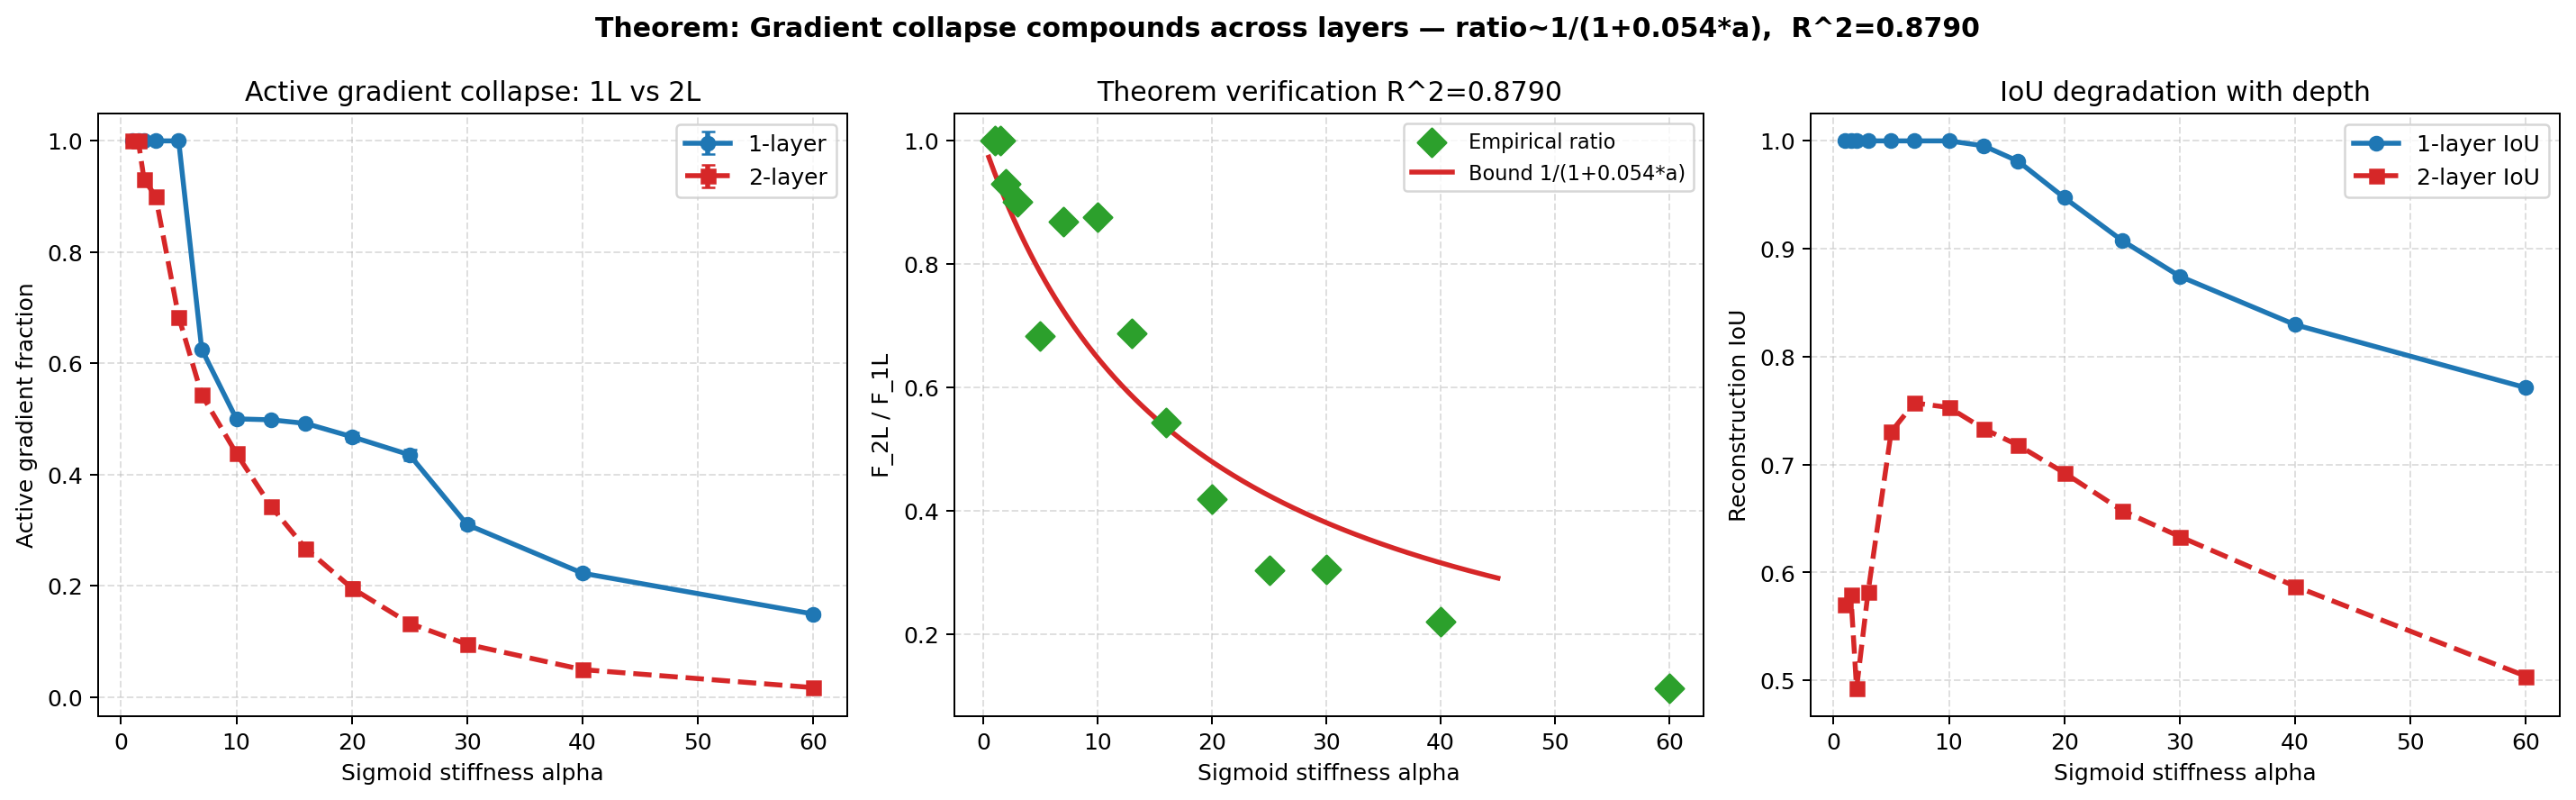
\includegraphics[width=0.85\linewidth]{theorem_verification.png}
\caption{Gate independence test for Theorem~\ref{thm:compound}. (Left) Mean
Pearson correlation between $\Gamma^{(1)}$ and $A_2^\top\Gamma^{(2)}$ at
convergence across $\alpha$ values. (Right) Distribution of correlations across
all seeds and $\alpha$ values. No seed exceeds $|\mathrm{corr}|=0.50$.}
\label{fig:gate_independence}
\end{figure}

The independence assumption underlying Theorem~\ref{thm:compound} is
empirically tested, not simply assumed. Mean $|\mathrm{corr}(\Gamma^{(1)},
A_2^\top\Gamma^{(2)})|=0.201$ across all tested configurations; no seed at
any $\alpha$ exceeds $|\mathrm{corr}|=0.50$. The gates are weakly correlated
rather than independent, introducing a small positive bias in the predicted
compounding rate, and---as stated at Theorem~\ref{thm:compound}---this is
why the theorem's validity is scoped to $\alpha\geq16$ rather than presented
as unconditional.

\paragraph{Discussion (Synthetic Setting).}

Three cross-cutting observations emerge from the synthetic fixed-kernel
setting. First, increasing $\alpha$ induces implicit dimensional collapse:
stable rank collapses $6.7\times$ from $\alpha=1$ (46.8) to $\alpha=60$
(6.9). Second, high-$\alpha$ regimes produce characteristic failure modes:
the optimiser stalls in flat plateaus, and sensitivity to initialisation
grows sharply (rising variance in Fig.~\ref{fig:convergence}). Third,
edge-driven dynamics: the gradient gate is active only when $Ax\approx c$,
corresponding to edge-like transition regions; early iterations reconstruct
coarse boundaries while later iterations fill interior regions.

Connection to compressed sensing: when $F_\alpha(x^*)\cdot N<\mathrm{rank}(A)$,
the effective system is underdetermined and recovery fails almost surely. This
suggests applying RIP-based guarantees from CS theory by treating the active
support as the effective measurement set~\cite{donoho2006compressed}.



\newpage
\input{checklist.tex}

\end{document}
